%% 
%% Copyright 2007, 2008, 2009 Elsevier Ltd
%% 
%% This file is part of the 'Elsarticle Bundle'.
%% ---------------------------------------------
%% 
%% It may be distributed under the conditions of the LaTeX Project Public
%% License, either version 1.2 of this license or (at your option) any
%% later version.  The latest version of this license is in
%%    http://www.latex-project.org/lppl.txt
%% and version 1.2 or later is part of all distributions of LaTeX
%% version 1999/12/01 or later.
%% 
%% The list of all files belonging to the 'Elsarticle Bundle' is
%% given in the file `manifest.txt'.
%% 

%% Template article for Elsevier's document class `elsarticle'
%% with numbered style bibliographic references
%% SP 2008/03/01

%% \documentclass[preprint,review,12pt]{elsarticle}

%% Use the option review to obtain double line spacing
%% \documentclass[authoryear,preprint,review,12pt]{elsarticle}

%% Use the options 1p,twocolumn; 3p; 3p,twocolumn; 5p; or 5p,twocolumn
%% for a journal layout:
%% \documentclass[final,1p,times]{elsarticle}
%% \documentclass[final,1p,times,twocolumn]{elsarticle}
%% \documentclass[final,3p,times]{elsarticle}
%% \documentclass[final,3p,times,twocolumn]{elsarticle}
%% \documentclass[final,5p,times]{elsarticle}
\documentclass[final,5p,times,twocolumn]{elsarticle}

%% For including figures, graphicx.sty has been loaded in
%% elsarticle.cls. If you prefer to use the old commands
%% please give \usepackage{epsfig}

\usepackage[utf8]{inputenc}
\usepackage[T1]{fontenc}
\usepackage{algorithm}
\usepackage{algpseudocode}

\usepackage{amssymb}
\usepackage{amsmath}
\usepackage{amsthm}
\usepackage{amssymb}

\usepackage{graphicx}
\usepackage{caption}
\usepackage{subcaption}

\usepackage{todonotes}

\graphicspath{{figures/}{./}}
%% The lineno packages adds line numbers. Start line numbering with
%% \begin{linenumbers}, end it with \end{linenumbers}. Or switch it on
%% for the whole article with \linenumbers.
%% \usepackage{lineno}

\journal{Computers and Geosciences}

\begin{document}

\begin{frontmatter}

%% Title, authors and addresses

%% use the tnoteref command within \title for footnotes;
%% use the tnotetext command for theassociated footnote;
%% use the fnref command within \author or \address for footnotes;
%% use the fntext command for theassociated footnote;
%% use the corref command within \author for corresponding author footnotes;
%% use the cortext command for theassociated footnote;
%% use the ead command for the email address,
%% and the form \ead[url] for the home page:
%% \title{Title\tnoteref{label1}}
%% \tnotetext[label1]{}
%% \author{Name\corref{cor1}\fnref{label2}}
%% \ead{email address}
%% \ead[url]{home page}
%% \fntext[label2]{}
%% \cortext[cor1]{}
%% \address{Address\fnref{label3}}
%% \fntext[label3]{}

\title{Selecting scenarios in temporal ensembles}

\author{Guilherme G. Schardong$^1$, Simone D. J. Barbosa$^1$, Waldemar Celes$^1$, \\
Regis Kruel$^2$, Alexandre Emerick$^2$, Luciano Reis$^2$, Ricardo Chaves$^2$ and H\'{e}lio Lopes$^1$}
%% use optional labels to link authors explicitly to addresses:
%% \author[label1,label2]{}
%% \address[label1]{}
%% \address[label2]{}

%% \author{}

\address{$^1$Departamento de Inform\'{a}tica - PUC-Rio\\
$^2$PETROBRAS\\}

\begin{abstract}
When dealing with large ensemble datasets, their sheer size may hinder any analysis necessary to extract knowledge from them. To solve this problem a number of selection approaches have been proposed. We propose an approach based on a score function for time series ensembles, along with a novel graphical tool, the rank chart, to evaluate a time series adherence to a reference series. We compare our results with a manual selection using a brushing and linking framework and with a $k$ Nearest Neighbors based selection of the series after projecting them using a Multidimensional Scaling algorithm. To evaluate our approach, we applied it to an oil reservoir ensemble in order to find the models with the best adherence to a set of reference time series. The results of our case study indicate that the proposed score function attained good results in the ranking of the time series and the rank chart proved to be an invaluable tool to analyze the behavior of the selected series compared to a reference set.
\end{abstract}

\begin{keyword}
  Representative Model Selection
  \sep Ensemble Methods
  \sep Time Series Processing
  \sep Brushing and Linking
  \sep Multidimensional Scaling
\end{keyword}

\end{frontmatter}

%% \linenumbers

%% main text

%%%%%%%%%%%%%%%%%%%%%%%%%%%%%%%%%%%%%%%%%%%%%%%%%%%%%%%%%%%%%%%%%%%%%%%%%%%%%%

\section{Introduction}
\label{sec:introduction}
Recent developments in simulation techniques have helped researchers better understand and predict several naturally occurring phenomena, ranging from weather forecast \cite{noodles-sanyal:2010} to circuit calibration \cite{lee:2010} and fluid dynamics \cite{hummel:2013}. These simulations produce an ever increasing amount of data, due to the availability of computing power and simulation model refinements. To extract any meaningful information from this amount of data, researchers have been developing an array of approaches in the most diverse areas: from data mining \cite{wang:2014}, to machine learning \cite{yang:2007}, visualization \cite{phadke:2012} and optimization \cite{alrefaei:2007}. Such approaches usually involve ways to better summarize the results using statistical measures, or ways to reduce the dimensionality of data and find meaningful entities that can represent the ensemble.

The recent introduction of ensemble methods in the oil industry has made it possible to apply several of these approaches to solve existing problems, such as: history matching \cite{aanonsen:2009}, enhance production forecasts \cite{wen:2005}, and improve strategical planning for oil reservoirs \cite{aanonsen:2009, chen:2009}. One of the key tasks in reservoir management is to develop a production strategy to be implemented \cite{schiozer:2004}. A production strategy consists of a set of wells, transmission lines, manifolds and a schedule with the activation times for each device in the oil reservoir \cite{meira:2016}. When such strategy is defined, it must be thoroughly analyzed to evaluate its profitability. A widely adopted approach to evaluate the profitability of a production strategy is to couple it with the reservoir model and the geological model and simulate the strategy's performance \cite{meira:2016}. Due to uncertainties inherent of the geological model, this process usually generate dozens up to hundreds of possible outcomes for each strategy.

Steagall and Schiozer \cite{steagall:2001} propose the use of three classes of models to evaluate the performance of a production strategy: a pessimistic, median and optimistic models with respect to the Net Present Value (NPV). Schiozer et al. \cite{schiozer:2004} improved the approach by requiring that the models selected be representative in other properties, such as Cumulative Oil Production (NP), Cumulative Water Production (WP) and Oil Recovery Factor (ORF) as well.

However the process of selecting this subset is a challenging task due to the sheer number of possible outcomes of a simulation and the constraints that need to be satisfied. Several approaches have been proposed to accomplish this task, ranging from optimization based approaches, to clustering and classification. We propose an approach that takes into account a range of time from each simulation and rank its outcomes according to a score function detailed below. We also propose a novel time series visualization tool to help analyze the adherence of each series the a set of percentile curves (P$_{10}$, P$_{50}$ and P$_{90}$) calculated from the simulations, as proposed by Stegall and Schiozer \cite{steagall:2001}.

%A common approach to compare the performance of different strategies is to select a subset of simulated models for each strategy, composed of optimistic, median and pessimistic models, and directly compare these models between the different strategies.

%The process of strategy evaluation then requires that a subset of these results be chosen in order to estimate the optimistic, median and pessimistic production rates.

\subsection{Objectives}
The goal of this work is to propose a novel approach for the visualization and selection of representative elements in an ensemble. To this end, we developed a novel visualization technique, the Rank chart, to graph the rank of the distances between each time series of the ensemble and a reference series. We also developed a score function in order to automatically select a subset of possible representative models for the ensemble. Other well established techniques, such as the Fan chart, Scenario/Distance chart and classic Multidimensional Scaling (MDS) are also employed to evaluate the visual results of the selection. We compared the results of our proposed approach to a set of series manually selected using the brushing \& linking technique, and also the closest series after a projection using the MDS algorithm. The main questions answered by our work are:

\begin{itemize}
  \item How does our approach compare to other, well established approaches found in the literature?
  \item How does our approach compare to a set of manually selected series? And to a set of series selected after applying a dimensionality reduction algorithm?
  \item Does the rank chart help unearth any information regarding the closeness of a model to a reference?
\end{itemize}

\subsection{Contributions}
The main contribution of our work is the proposal of a representative selection approach that handles time series data as a whole, not only a single time step, as most approaches found in the literature \cite{selection-sarma:2013, meira:2016}. Another contribution is the development of a new visualization technique, named Rank chart, to help analyze the behavior of the time series compared to a reference. The main contributions of our work may be summarized as follows:

%The main contribution of this work is the proposal of a new visualization technique to help on the analysis and selection of representative elements in an ensemble of time series. We propose a score based automatic selection of possible representatives and compare it against a manual selection assisted by both a scenario/distance chart and an Multidimensional Scaling algorithm. For the manual selection, we employ the brushing and linking technique to highlight the selected entities with the other visualization tools employed. The main contribution of our work can be summarized as follows:

\begin{itemize}
  \item Proposal of a score selection approach that uses a range of values from each time series;
  \item Proposal of a novel graphical tool, the Rank Chart, for the analysis of time series adherence and behavior against a reference;
  %\item Comparison of three different selection methods: a score approach, smallest distance selection and closest projected points selection to evaluate the results of our approach.
\end{itemize}

The remainder of this paper is organized as follows: Section \ref{sec:rel-work} presents related works grouped by topic: Ensemble Visualization and Representative Model Selection. Next, in Section \ref{sec:tools} we introduce the main components of the proposed framework and explain the visualization and interaction techniques used. Section \ref{sec:experiments} presents an experiment based on a real world ensemble used to test our approach. Section \ref{sec:discussion} presents the comparisons of our results with other approaches found in the literature. Finally, Section \ref{sec:conclusion} presents some concluding remarks and directions for future work.

%%%%%%%%%%%%%%%%%%%%%%%%%%%%%%%%%%%%%%%%%%%%%%%%%%%%%%%%%%%%%%%%%%%%%%%%%%%%%%

\section{Related Work}
\label{sec:rel-work}
We have divided the related works in two categories: Ensemble Visualization and Representative Model Selection. Our work makes use of Multidimensional Projection (MP) techniques to help visualize the proximity between models in the ensemble, therefore, we have included some works related to this area as well.

\subsection{Ensemble Visualization}
An ensemble is, by definition, a collection of related datasets, where each entity is usually composed by multidimensional, multivariate data. An ensemble can be generated, for example, by running several simulation rounds with different input parameters to analyze the behavior of complex systems \cite{noodles-sanyal:2010}.

The analysis and visualization of such data is a daunting task due to their high complexity and dimensionality. As a result, there are several published approaches to accomplish these tasks \cite{phadke:2012, hlawitschka:2013, ensemblevis-potter:2009, multicharts-demir:2014}. In particular, Potter et al. \cite{ensemblevis-potter:2009} proposed the development of a framework for statistical visualization of bidimensional weather ensembles. The work of Demir et al. \cite{multicharts-demir:2014} proposed a technique for the interactive visual exploration of tridimensional scalar ensembles using brushing and linking, in addition to line and bar charts of statistical data measures.

Since the areas of ensemble and uncertainty visualization are related, several techniques can be applied in both areas. Chen \cite{uncert-proj-chen:2015} proposes a multidimensional projection of ensemble data that takes into account the data means and distributions. Sanyal et al. \cite{noodles-sanyal:2010} proposed a tool to visualize numerical uncertainty in weather models by plotting iso-lines, ribbons and glyphs over map areas with high weather uncertainty.

\subsection{Representative Model Selection}
The task of analyzing and retrieving meaningful knowledge from a large ensemble is incredibly complex, if not intractable. This only gets worse as the models used for generating the ensembles, and the simulators themselves, are improved and refined. Therefore, there is a need for the development of approaches to reduce the amount of data to be analyzed. Some of the more recent methods were derived from MP algorithms \cite{uncert-proj-chen:2015, mp-wong:2013, lamp-joia:2011}. This approach provides a good visual representation of the similarity between ensemble entities. The uncertainty information may also be taken into consideration during the projection, as in the work of Chen et al. \cite{uncert-proj-chen:2015}. Joia et al. \cite{lamp-joia:2011} propose a projection algorithm that uses a reduced set entities as control points and manually positions them in the projection space to guide the process for the remaining entities. This approach allows the user to establish correlations between the control points and visualize their relationships with the remaining elements of the ensemble. Wong et al. \cite{mp-wong:2013} propose the reformulation of several MP algorithms to preserve temporal coherence during the projection of volumetric, time varying data with interesting results.

Another possible approach is to choose a representative subset of the original ensemble to perform the analysis. The process of reducing the available data incurs in a potential loss of information, which would be detrimental for analysis. Therefore, the set of elements chosen must be representative of the ensemble in order to execute certain analysis tasks and generalize the conclusions to the whole ensemble. A first possible approach to solve this problem is to apply clustering algorithms using the ensemble as input and selecting the entities closest to the cluster centers as representative \cite{lee:2010}. There is also the possibility of applying a $k$ Nearest Neighbors (kNN) approach and select a number of models most similar to the references according to an arbitrary distance metric.

More recently, this selection has been addressed as an optimization problem, where the goal is to maximize, or minimize, an objective function. In this context, Sarma et al. \cite{selection-sarma:2013} modeled the selection as a constrained minimax combinatorial optimization problem and solved it by doing an exhaustive search over the solution space for small ensembles and by employing a greedy algorithm to search for a solution in larger ensembles. Their approach reportedly performs faster and is more accurate than clustering approaches. Meira et al. \cite{meira:2016} employed the same approach to select a set of representative models that minimizes a multi-objective cost function composed by a risk curve factor, an attribute-level coverage factor and a weighted cross plot spread factor. By minimizing this function, Meira's approach selects high quality sets of representative models without optimistic or pessimistic biases.

The works of Sarma et al. \cite{selection-sarma:2013} and Meira et al. \cite{meira:2016} show that the optimization approach for selecting a set of models obtains promising results while maintaining a good computational performance. However, both approaches use simulation parameters not accessible in our experiments, making the task of comparing their approach to ours impossible.

Our approach uses only data resulting from the simulations, and while we used scenarios from the oil \& gas industry, our technique can be easily adapted to other areas with similar requirements.

%OBJECTIVE FUNCTION - minimize the weighted euclidean distance of the selected models and the reference percentiles. The weights are composed by the score function%

%\subsection{Brushing and Linking}
%The visual analysis of ensemble data usually requires several different graphical tools to be successful. These tools must work in conjunction to help the user draw feasible conclusions from the data. Brushing and Linking \cite{brush-becker:1987, link-buja:1991} has proved to be and invaluable technique to achieve this goal. As a result, several frameworks for ensemble and uncertainty analysis have been proposed with a brushing and linking component as its central piece [[CITATIONS HERE]]. The work of Demir et al. \cite{multicharts-demir:2014} makes use of this technique by allowing the user to select interesting regions in a line/bar chart view while highlighting the corresponding cells in a tridimensional view of the data. Chen et al. \cite{uncert-proj-chen:2015} uses brushing and linking for selecting points of interest in a bidimensional projection of the ensemble data and showing the geo-location, uncertainty histogram and parameters of the brushed points. Potter et al. \cite{ensemblevis-potter:2009} allows the brushing of geographical regions in a bidimensional view and shows quartiles and filmstrip summary views of the ensemble.

%%%%%%%%%%%%%%%%%%%%%%%%%%%%%%%%%%%%%%%%%%%%%%%%%%%%%%%%%%%%%%%%%%%%%%%%%%%%%% 

\section{Tools and Techniques}
\label{sec:tools}
This section describes the techniques developed and employed in our work.

\subsection{Objective Function}
\label{sec:obj_func}
In order to select the representative models, we must define the criteria they must satisfy. The desired models must be close to a set of reference models selected by the user. The traditional approach uses the percentiles 10, 50 and 90 (henceforth called P$_{10}$, P$_{50}$ and P$_{90}$, respectively) models calculated from the ensemble as references. These models represent the optimistic, median and pessimistic production estimates. The measure of "closeness" between the scenarios is defined as the euclidean distance between the production curves at each simulation time step.

The euclidean distance may be used as a criterion for selection. In this case, our goal would be to select models that minimize the euclidean distance to each reference model. However, if this method was adequate, then clustering, or kNN approaches would perform well, since several of them use the euclidean distance between the entities. Therefore, we propose an objective function based on a score calculated for each curve, along with the euclidean distance to rank the models by their adherence to the reference models, instead of solely based on their distance.

Given the absolute ranking calculated based on the euclidean distance between the entities, we assign a score for each possible rank. For an ensemble of $N$ entities, we use a linear function $f(r) = N - r - 1$, where $\left(r \in \mathbb{N} | r \in [1, N] \right)$ as the score for each rank $r$. We also assign a weight for each simulation time step based on the desired adherence between the candidate models and the references. The definition of this function depends on the type of analysis and behavior of the ensemble itself. Algorithm \ref{alg:rank-score} shows how we calculate the score $s$ of each entities in the ensemble given the absolute ranking $R$ of each element.

%\begin{algorithm}
%  \caption{Rank score algorithm}
%  \begin{algorithmic}[1]
%    \Procedure{RankScore}{$R, S, W$}
%    \State // R is the absolute ranking matrix of (number of time steps, number of curves) dimensions
%    \State // S is the array of scores for each possible ranking
%    \State // W is the weights of each time step
%    
%    \For {$r \in [1, $ncol$(R)]$}
%    \State $s(r) \gets 0$
%    \State $rank \gets R(r, :)$
%    \For {$t \in [1, $length$(rank)]$}
%    \State $s(r) \gets s(r) + W(t) \times S(rank(t))$
%    \EndFor          
%    \EndFor
%    
%    \Return $s$
%    \EndProcedure
%  \end{algorithmic}
%  \label{alg:rank-score}
%\end{algorithm}

\begin{algorithm}
  \caption{Rank score algorithm}
  \begin{algorithmic}[1]
    \Procedure{RankScore}{$R$}
    \State // R is the absolute ranking matrix of (number of time steps, number of elements) dimensions
    
    \For {$r \in [1, $ncol$(R)]$}
    	\State $s(r) \gets 0$
	    \State $rank \gets R(r, :)$
	    \For {$t \in [1, $length$(rank)]$}
	    	\State $s(r) \gets f(r) + w(t) \times S(rank(t))$
	    \EndFor          
    	\EndFor
	
        \State \Return $s$
    \EndProcedure
  \end{algorithmic}
  \label{alg:rank-score}
\end{algorithm}

\subsection{Rank Chart}
\label{sec:rank}
When searching for meaningful entities in an ensemble there is usually a synthetic ideal entity used as reference, and the task is to select the ensemble entity that most closely resembles the reference. Such task is relatively simple when dealing with two or three dimensional points and can be automated by a kNN algorithm. However, selecting the most similar entities in an ensemble composed of time series can be a daunting task. With this kind of data, the user may search for a series that closely matches the reference in a number of key time steps, or that minimizes an objective function based on the reference. To help with this task, a novel type of visualization is proposed: the Rank Chart. This chart graphs the ranking of ensemble elements against a reference, along the time axis.

The rank chart is built by iterating through the time steps of the ensemble entities and calculating the distance between each series and the reference up to that step. This distance is then ordered in ascending order and ranked accordingly. This process creates a new set of time series, now composed of the absolute ranks attained by each ensemble entity at each time step. These ranks are then plotted in a two-dimensional plane where the $X$ axis is the time step and the $Y$ axis is the rank. An example of a rank chart is shown in Figure \ref{fig:rank-sample}.

\begin{figure}[H]
  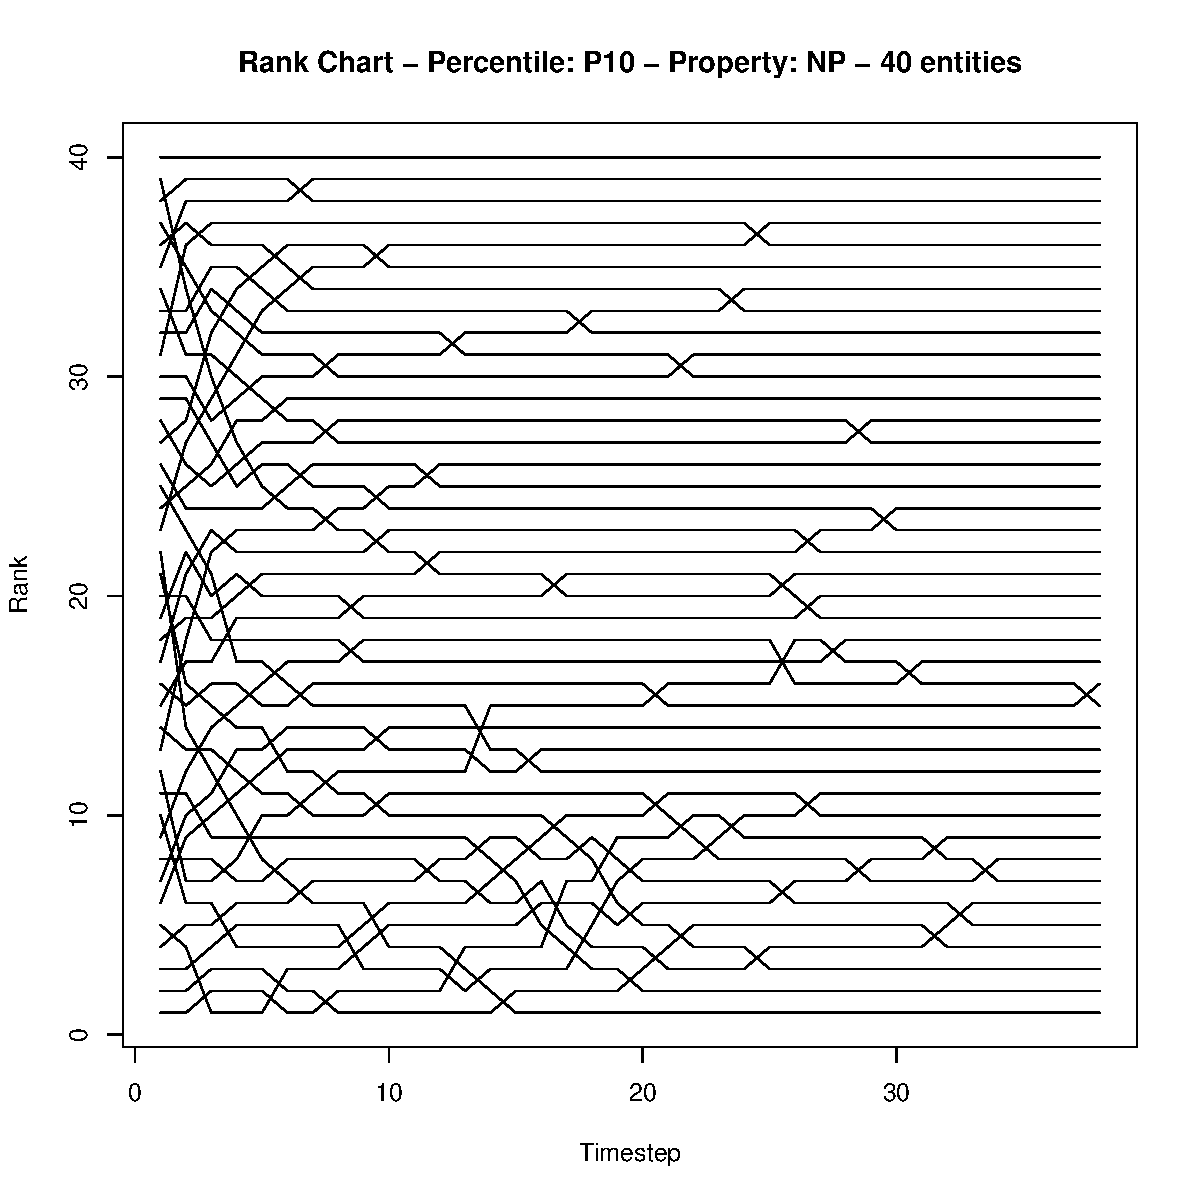
\includegraphics[width=\columnwidth]{rank-sample-40.pdf}
  \caption{Rank chart of 40 ensemble elements using the P$_{10}$ curve as reference.}
  \label{fig:rank-sample}
\end{figure}

Figure \ref{fig:rank-sample} shows the absolute rankings of each time series compared against a reference series. As the size of the ensemble grows, the chart will be further affected by visual clutter, making the process of selecting the most adherent series a difficult one. To solve this problem, we use the objective function proposed in Section \ref{sec:obj_func} and select the $k$ series with the highest score. The results of this selection are shown in Figure \ref{fig:rank-score-sample}. The time step weight function used was: $w(t) = arctan(t)$, where $t$ is the time step index and the 5 highest scored curves are marked in shades of green. Figure \ref{fig:rank-score-brush} shows the rank chart of the curves selected using the brushing and linking technique; the selected curves are also colored in tones of green.

%An approach to reduce the number of possible candidates is then proposed. From the absolute ranking used to plot the chart, a score for each series can be calculated by assigning a value for each possible rank and, optionally, a weight for each time step. The overall score is calculated by accumulating the values of each rank weighted by the time step value. Algorithm \ref{alg:rank-score} shows how this score is calculated.

%\begin{figure}[H]
%	\centering
%	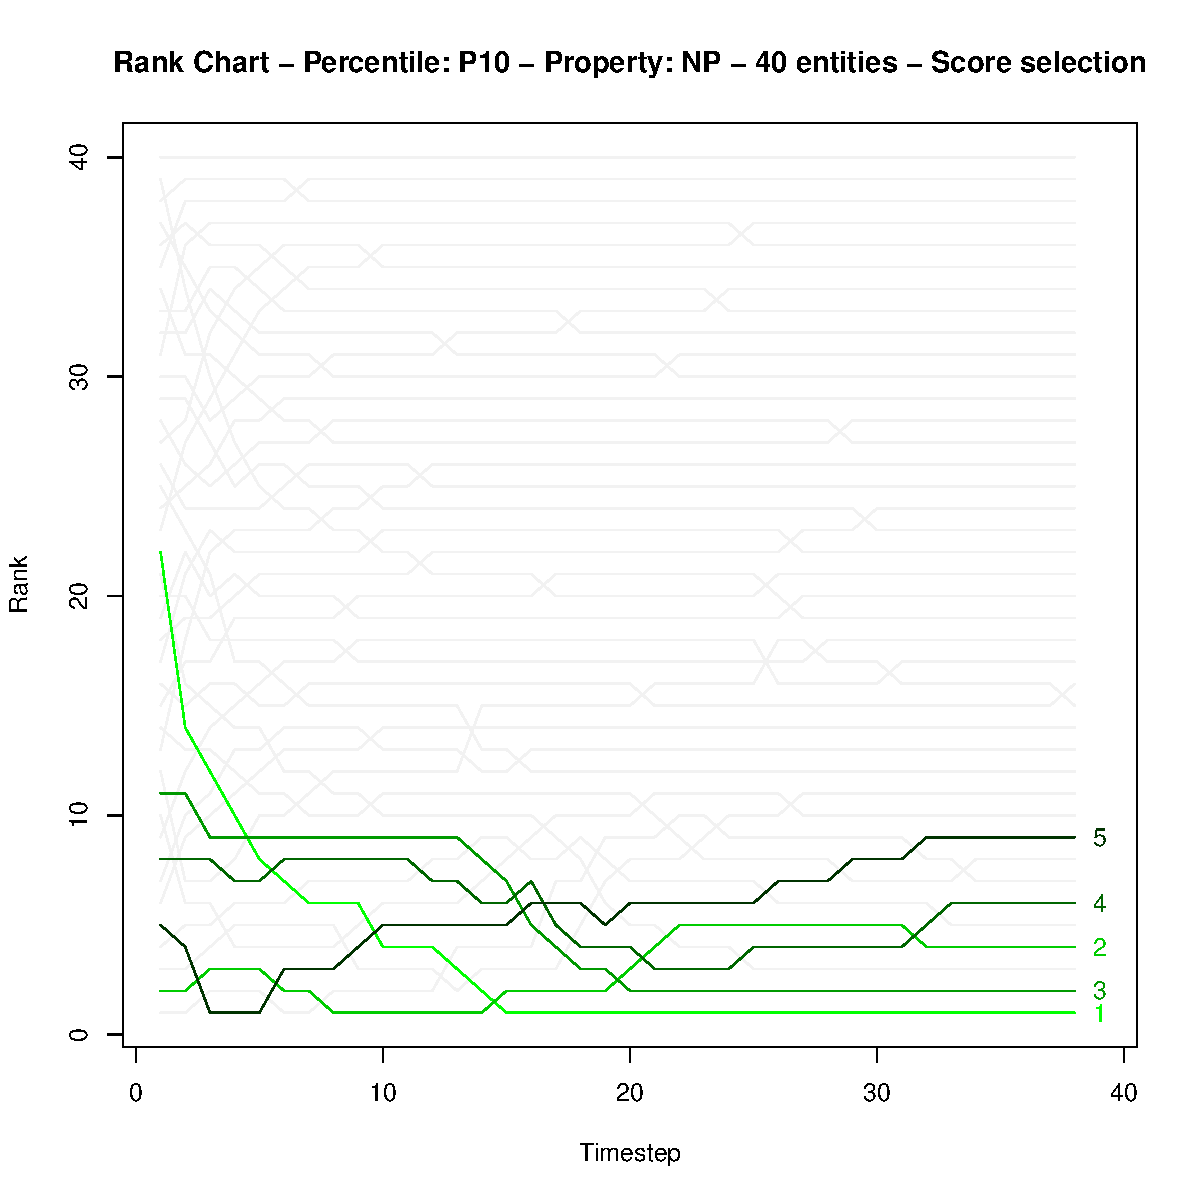
\includegraphics[width=\columnwidth]{rank-score-40.pdf}
%	\caption{Rank chart of 40 ensemble elements using the percentile 10 curve as reference. The 5 best ranked curves according to the scoring algorithm are highlighted from green to black.}
%	\label{fig:rank-score}
%\end{figure}

%To plot this chart, an approach to rank the time series must be defined beforehand. The proposed approach uses the euclidean distance between the ensemble series and the reference as a first measure of ranking. At each time step, the distance between each series and the reference is calculated and sorted in increasing order. This first step produces a new set of time series composed by their absolute ranking at every time step analyzed. From this first ranking, a score is calculated by assigning a value for each rank and, optionally, a weight for each time step. Algorithm \ref{alg:ranking} shows how the rank is calculated. The curves with a highest score are then highlighted in the rank chart for analysis.

\begin{figure}[H]
  \begin{subfigure}[b]{0.48\columnwidth}
    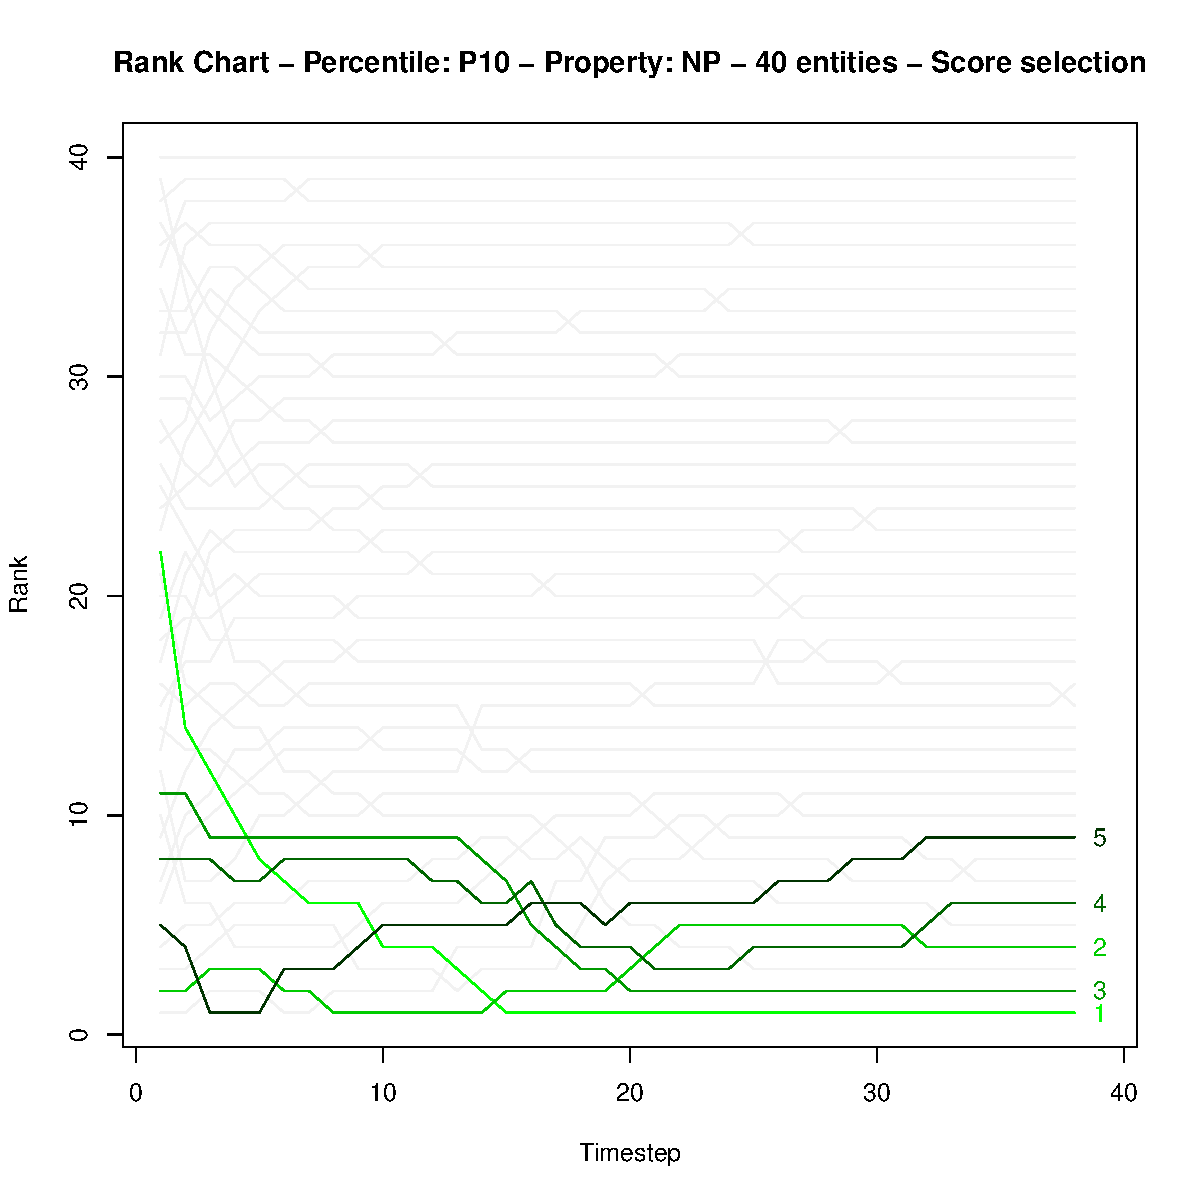
\includegraphics[width=\columnwidth]{rank-score-40.pdf}
    \caption{The highest scoring curves highlighted are: UNISIM\_11, UNISIM\_17, UNISIM\_13, UNISIM\_28, UNISIM\_10.}
    \label{fig:rank-score-sample}
  \end{subfigure}
  ~
  \begin{subfigure}[b]{0.48\columnwidth}
    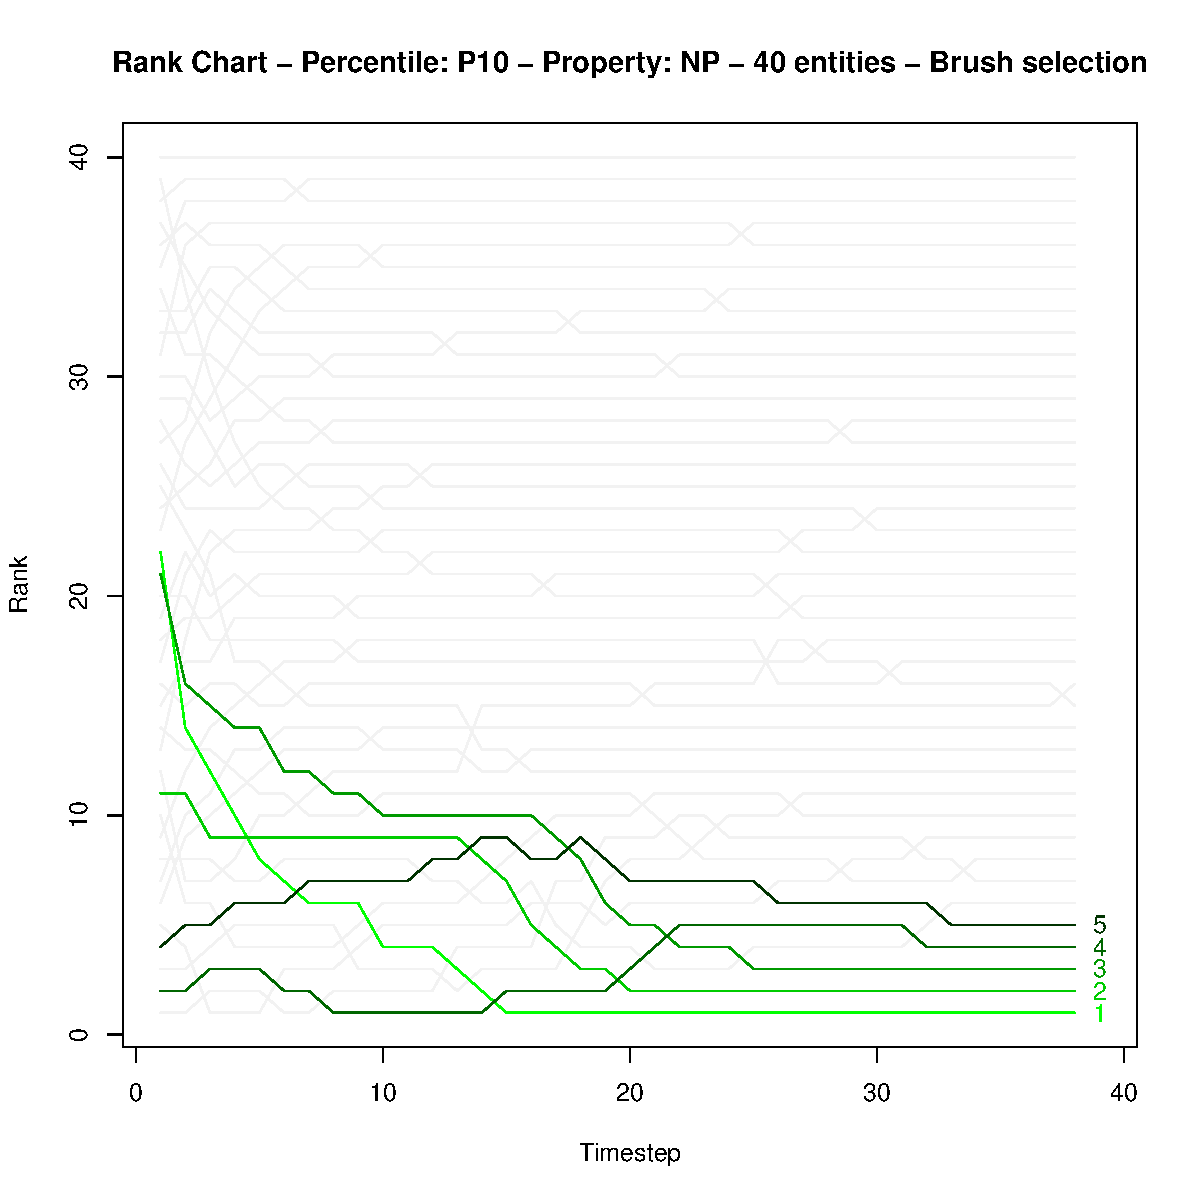
\includegraphics[width=\columnwidth]{rank-brush-40.pdf}
    \caption{The curves manually highlighted are: UNISIM\_11, UNISIM\_13, UNISIM\_35, UNISIM\_17, UNISIM\_24.}
    \label{fig:rank-brush-sample}
  \end{subfigure}

  \caption{Rank chart of 40 ensemble elements using the P$_{10}$ curve as reference. The 5 best ranked curves according to the scoring algorithm and the manual selection are highlighted from green to black. The numbers next to the curves indicate their overall ranking.}
  \label{fig:rank-score-brush}
\end{figure}

Figure \ref{fig:rank-score-brush} shows the rank charts of the NP property of 40 curves in our ensemble before the history matching process. Details about the ensemble are explained in Section \ref{sec:data}. The rank charts show the 5 best ranking curves selected by the proposed score algorithm and a manual brushing using the scenario chart, explained in Section \ref{sec:scen}, to mark the closest curves. Of the 5 selected curves, 3 were selected by both approaches and their behavior can be analyzed by using the rank chart. The NP curves of fields UNISIM\_11, UNISIM\_17 and UNISIM\_13 are highlighted in Figure \ref{fig:rank-highlight} for better viewing, their respective ranks according to the score approach are next to the curves.

\begin{figure}[H]
  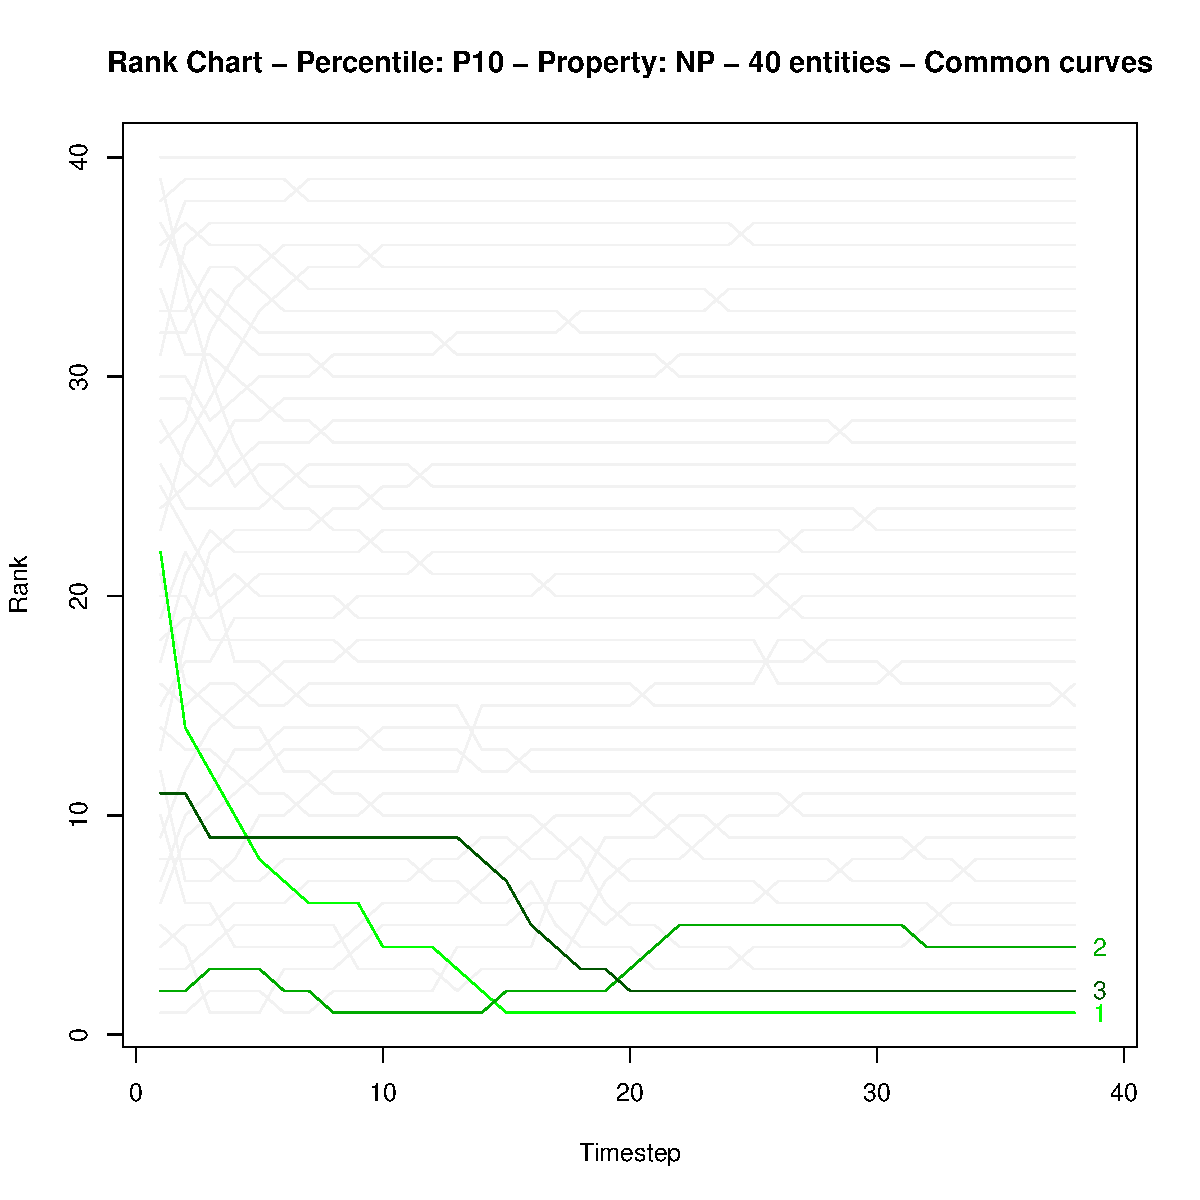
\includegraphics[width=\columnwidth]{rank-common-40.pdf}
  \caption{Rank chart of 40 ensemble elements using the P$_{10}$ curve as reference. The 3 common curves selected by the score approach and the manual brushing are highlighted from green to black. The numbers next to the curves indicate their overall ranking using the score approach.}
  \label{fig:rank-highlight}
\end{figure}

\subsection{Scenario/Distance Chart}
\label{sec:scen}
A task closely related to the one described in section \ref{sec:rank} is the search for an entity, or entities, closest to the reference. To accomplish this, a measure of closeness (or dissimilarity) must be defined beforehand. This step is highly dependent on the type of data and analysis task at hand, requiring intimate knowledge of both by the user for an appropriate choice. The next step in the process is to calculate the distance between each ensemble entity and the reference entity. In a normal process, the user would then select a number of most similar entities for further analysis. This choice of action overlooks an important source of information about the data, namely the way the distances (or similarities) are arranged and the potential patterns they may form.

To help solve this issue, another visualization technique is applied, the Scenario/Distance Chart. This chart graphs the distance of ensemble entities to a reference element. The $X$ axis represents the entity and the $Y$ axis is the distance between each entity and the reference. Figure \ref{fig:scen-chart-40} shows an example of a Scenario/Distance chart.

\begin{figure}[H]
  \begin{subfigure}[b]{0.48\columnwidth}
    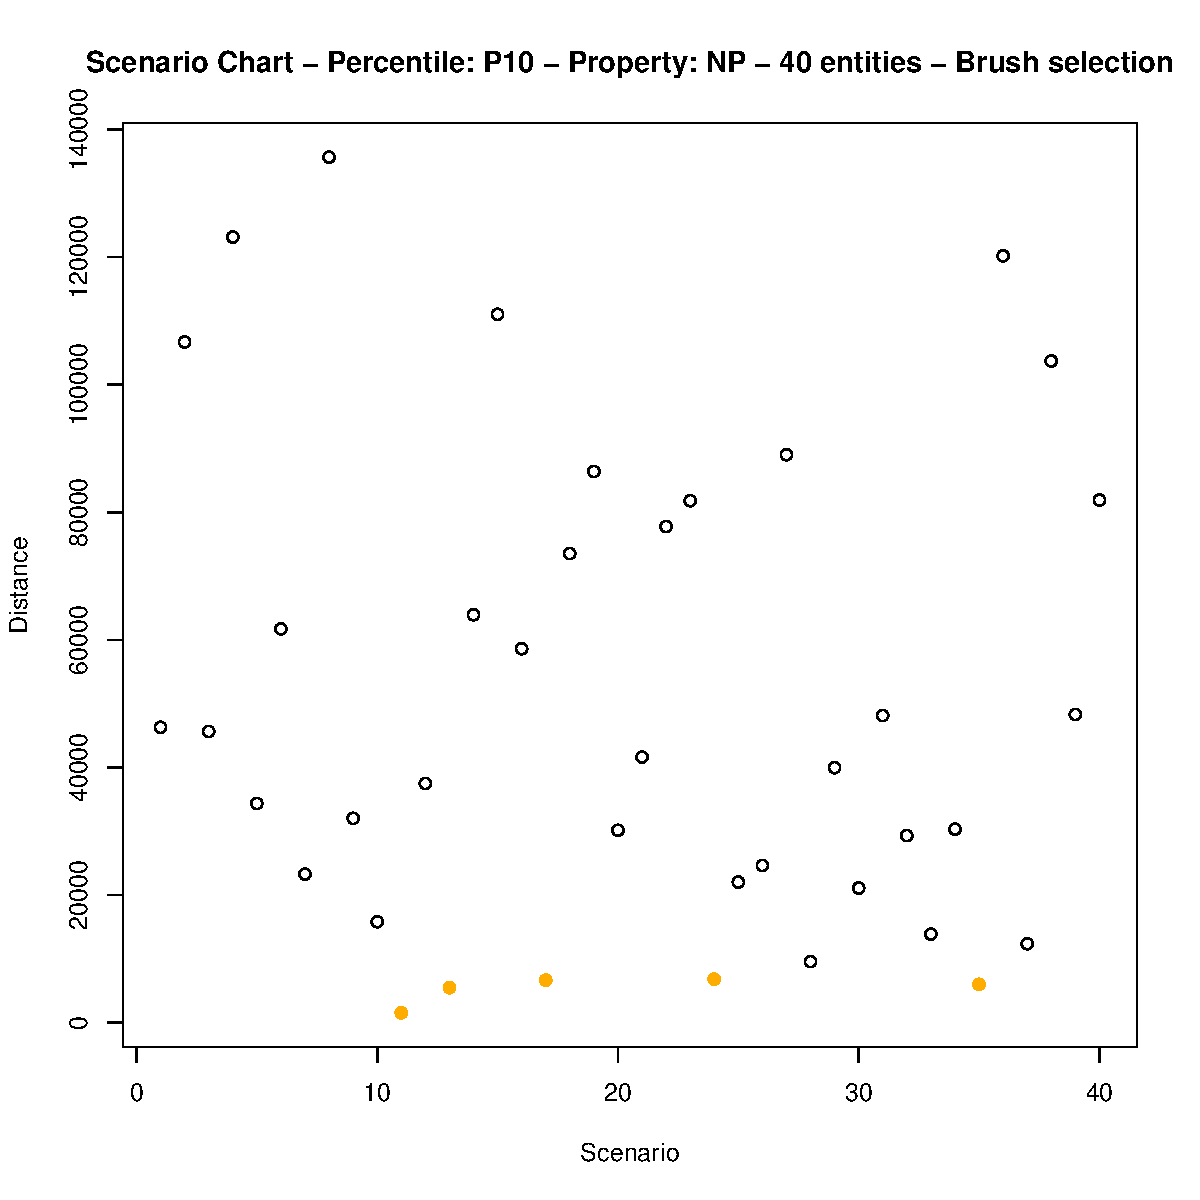
\includegraphics[width=\columnwidth]{scen-brush-40.pdf}
    \caption{Scenario/Distance chart with a decimal scale on the $y$ axis.}
    \label{fig:scen-brush-sample}
  \end{subfigure}
  ~
  \begin{subfigure}[b]{0.48\columnwidth}
    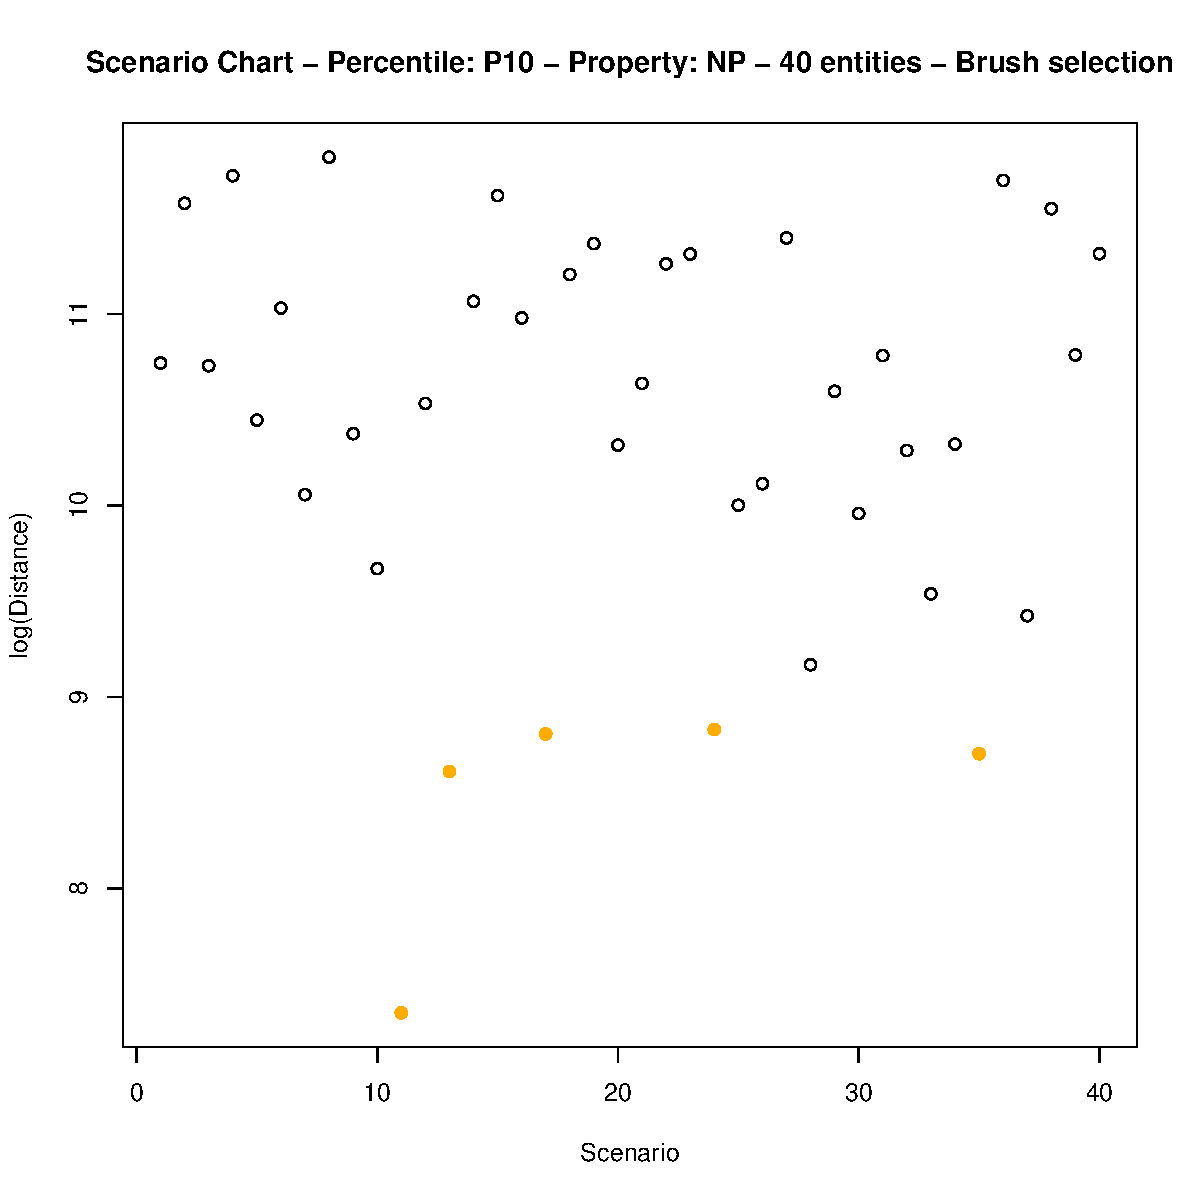
\includegraphics[width=\columnwidth]{scen-brush-40-log.pdf}
    \caption{Scenario/Distance chart using a logarithmic scale on the $y$ axis.}
    \label{fig:scen-brush-sample-log}
  \end{subfigure}

  \caption{Scenario/Distance chart of 40 ensemble elements using the P$_{10}$ curve as a reference. The 5 best ranked curves according to the manual selection are highlighted in orange.}
  \label{fig:scen-chart-40}
\end{figure}

The scenario chart can easily be adapted to graph similarities, or correlations between the reference and ensemble entities. The scenario chart can be used to highlight the closest scenario in the corresponding rank and fan charts using a brushing and linking approach. This approach provide a powerful tool for analysis of time series ensemble data.

%When used along with the brushing and linking component, the user is able to select scenarios at key distances for further inspection and they will be highlighted in other visualizations. Along with the rank chart, this provides a powerful tool for analysis of ensemble data and selection of key elements for further processing. 

%\section{Horizon Chart}
%\label{sec:horizon}
%
%A task commonly occurring in ensemble analysis is the visual comparison of time series. There are a number of visualization tools to help accomplish this task, such as line and overlaid line charts. As the number of series grows, this task becomes increasingly difficult, due to lack of screen space or cluttering. Both of these problems can be seen in Figure [[FIG HERE]].
%
%The Horizon Chart \cite{horizon-heer:2009} offers an approach to partially solve these issues. An horizon chart is a modified version of a line chart built by mirroring, assigning different colors to negative values and dividing the chart in bands. These modifications allows for the chart to occupy less than half the size of a line chart \cite{horizon-heer:2009}. A large number of time series can then be compared by stacking their charts and using the same scale and origin base line. Once this structure is understood, a user can rapidly establish patterns in the series' behavior or, spot outlier elements in the set \cite{ts-lamigueiro:2014}. Furthermore, the series can be compared against a common curve by using it as a base line. An example of a horizon chart is shown in Figure \ref{fig:horizon-ex}.
%
%\begin{figure}
%  \centering
%  %\includegraphics{}
%  \caption{Example of Horizon chart.}
%  \label{fig:horizon-ex}
%\end{figure}
%
%When the number of series grows, the horizon chart eventually suffers from the same problem of line charts, namely, lack of screen space. Instead of plotting all series available in the ensemble, a reduced subset of them can be selected. This is possible due to brushing and linking component employed in the proposed framework. After marking any interesting series in other tools, the horizon chart may be used to visualize them. Since the rank and scenario charts use a reference series for their processing, the same series can be used as a base line for a comparison between the behaviors of the selected series and the reference.

\subsection{Fan Chart}
\label{sec:fan}
Fan charts were originally developed by the Bank of England for their inflation forecasts in 1996 \cite{fanchart-britton:1998} and have become a standard way for visualizing uncertainty in such situations \cite{rfanplot-abel:2015}. While overlaid line charts enables the visualization of a whole ensemble, they suffer from the aforementioned cluttering problem. Fan charts avoid this by plotting only color coded statistically significant measures of the ensemble data, such as maxima, minima, standard deviations and percentiles. An overlaid line chart and the corresponding Fan Chart can be seen in Figure \ref{fig:spag-fan}.

\begin{figure}[H]
  \centering
  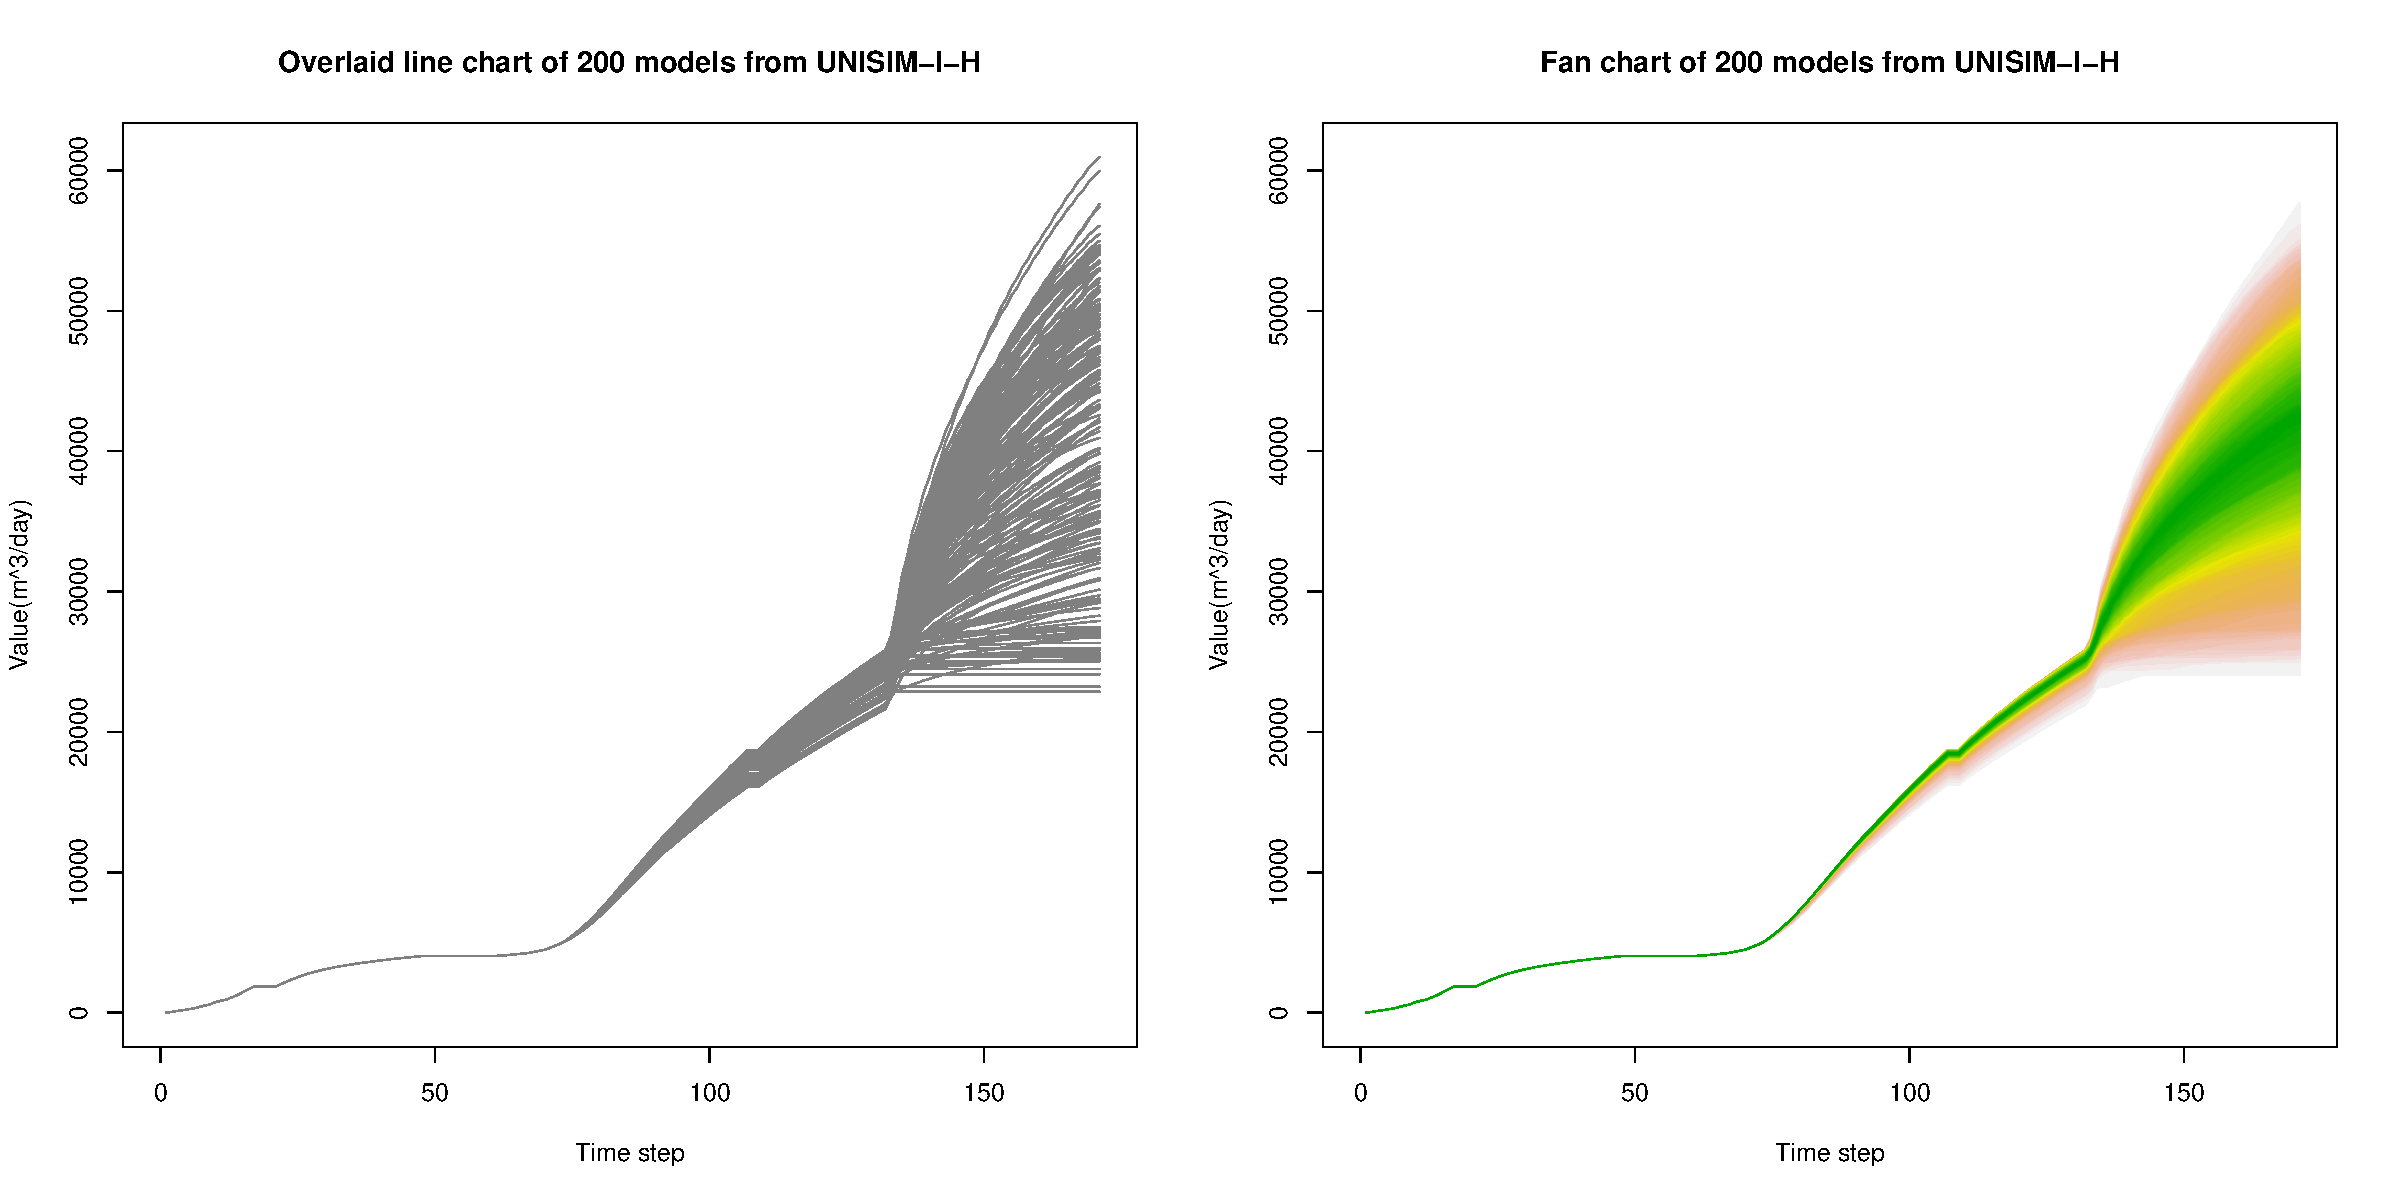
\includegraphics[width=\columnwidth]{line-fan.pdf}
  \caption{Visual comparison of an overlaid line chart and the corresponding fan chart using the whole time range (171 time steps) of 200 ensemble elements.}
  \label{fig:spag-fan}
\end{figure}

The Fan Chart has become a standard, well established visualization tool in several areas, such as finance \cite{celasun:2006}, demography \cite{gerland:2014}, climate science \cite{mcshane:2011} and genealogy \cite{genealogy-draper:2008}. Since our framework proposes to help during the analysis step of ensemble data, the fan chart is an invaluable tool to achieve this goal.

In order to compare the behavior of a subset of series to the whole ensemble, we plot the fan chart of the ensemble overlaid by the line charts of the aforementioned subset. This approach allows for a comparison of the selected series against the general behavior of the ensemble in a compact an simple way, with minimal visual clutter, as long as the number of selected series is relatively low. An example of this approach is shown in Figure \ref{fig:sel-ensemble}.

%In order to compare the behavior of the selected series to the whole ensemble, we plot the fan chart of the ensemble overlaid by the line charts of the selected series. This approach allows for a comparison of the selected series against the general behavior of the ensemble in a compact an simple way, with minimal visual clutter, as long as the number of selected series is relatively low. An example of this approach is shown in Figure \ref{fig:sel-ensemble}.

%In our use case there are basically two ways that the fan chart can be used. Both of them require the selection of a subset of time series. By using the brushing and linking component, a fan chart can be plotted with the brushed and reference series as input, therefore showing their behavior independently of the remaining data in the ensemble. The second approach involves the plotting of a fan chart featuring the whole ensemble, with any brushed series overlaid as line charts. This last approach allows for a comparison of the selected series against the general behavior of the ensemble in a compact an simple way, with minimal visual clutter. An example of both approaches is shown in Figure \ref{fig:sel-ensemble}.

%\begin{figure}[H]
%  \centering
  % \includegraphics{}
%  \caption{Two approaches to compare the selected series. The first compares just the series' behavior. The second compares the selected series with the whole ensemble.}
%  \label{fig:sel-ensemble}
%\end{figure}

\begin{figure}[H]
  \centering
  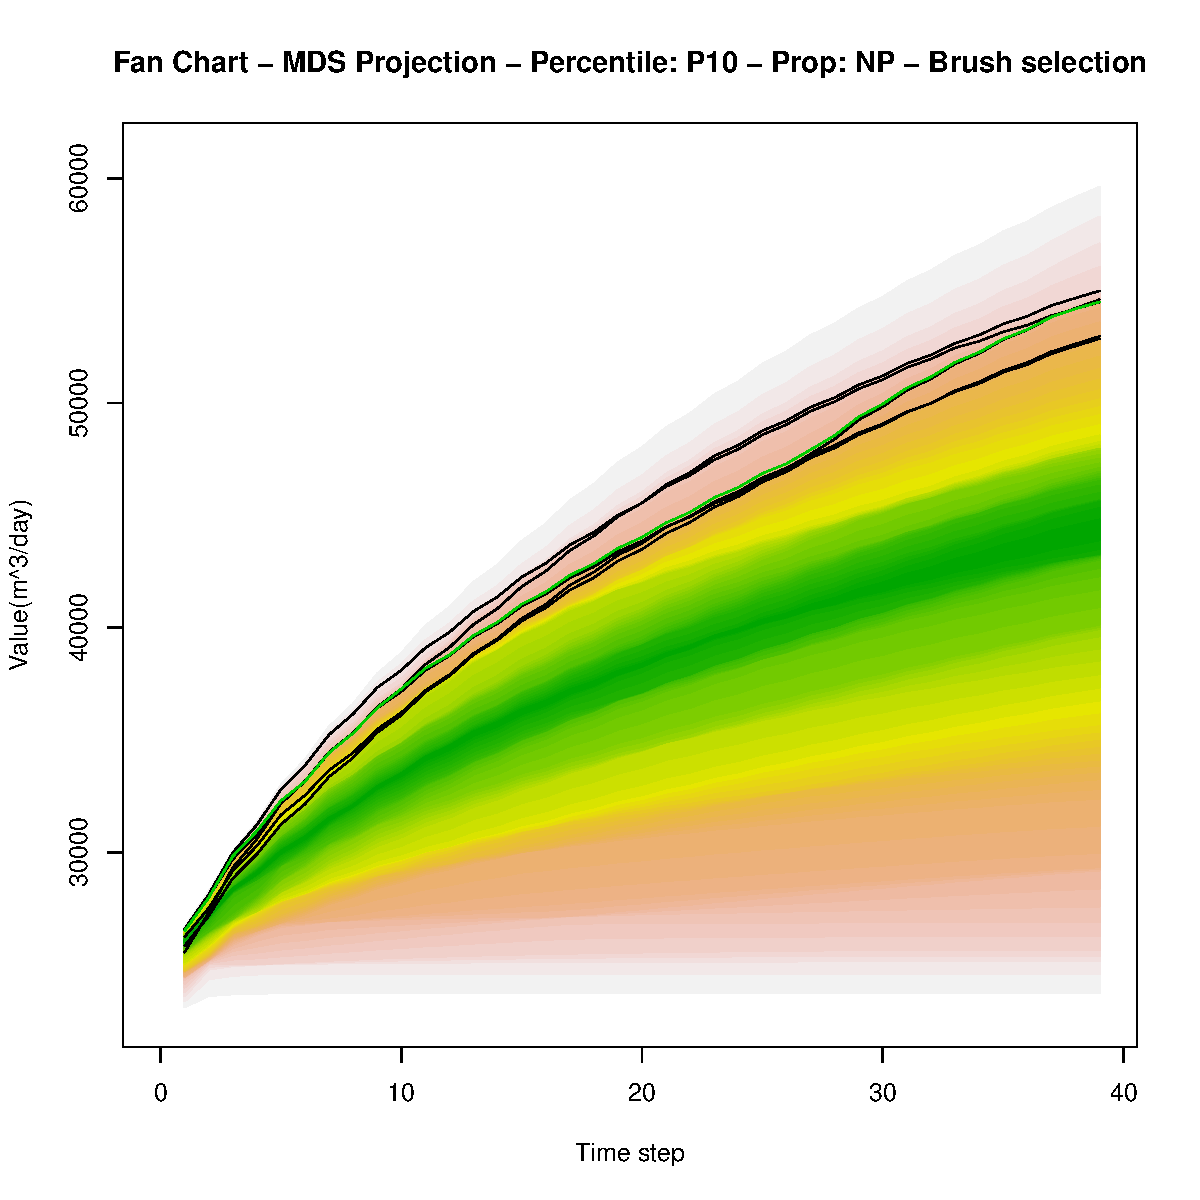
\includegraphics[width=\columnwidth]{fan-brush-40.pdf}
  \caption{Fan chart overlaid by the line charts of the series highlighted in Figure \ref{fig:rank-brush-sample} (in black) and the reference series (in green). Only the forecast data was used to generate this fan chart. The data used has a total of 171 time steps, the last 39 being the forecasts.}
  \label{fig:sel-ensemble}
\end{figure}

\subsection{Multidimensional Scaling}
\label{sec:mds}
Multidimensional Scaling is a set of techniques aimed at visualizing the information contained in a distance matrix \cite{kruskal:1978}. In the classical variant, the objects whose pairwise distances are represented in the input matrix $D$ are projected in an $N$-dimensional space where the euclidean distances $D_X$ between the resulting points $x_i \in X$ are approximately the same as in $D$. This technique may also be modeled as an optimization problem, where the algorithm attempts to minimize a strain, or stress function $s$ defined in terms of $D$ and the euclidean distance between the set of projected points $X$. Equation \ref{eq:stress-mds} gives an example of $s$.

\begin{equation}
s = \min_{x1, ..., x_I} \sum_{i < j} (||x_i - x_j|| - \delta_{i,j})^2  
\label{eq:stress-mds}
\end{equation}

The classical MDS algorithm provides the means to visualize high dimensional data in a lower dimensional space in a manner that preserves, as well as possible, the distances between entities. This facilitates the analysis of relationships between individuals. One important remark is that the number of dimensions $N$ has a direct effect on the preservation of the original distances. In general, larger values of $N$ produce smaller errors on the final projection.

An important property of the projected points is that they can be rotated and translated freely, as long as the distances between them are preserved. Such manipulations are often employed to fit the points in a set of meaningful axes to aid the interpretation of the results.

The classical MDS algorithm can be described by the following steps:

\begin{enumerate}
  \item Let $D_2$ be the squared distances $[d^2]$ in $D$;
  \item Let $B = -\frac{1}{2}J D_2 J$ be a double centered version of $D_2$ using the centering matrix $J = I - \frac{1}{n} \textbf{1}$;
  \item Extract the $N$ largest positive eigenvalues of $B$ and their corresponding eigenvectors;
  \item Let $\Lambda$ be the diagonal matrix with the $N$ largest eigenvalues of $B$ and let $E$ be the matrix with the corresponding eigenvectors. Let $P = E \times \Lambda^\frac{1}{2}$  be the projected coordinates.
\end{enumerate}

\noindent
A worked example can be found in Wickelmaier \cite{mds-wickelmaier:2003}.

\subsection{Brushing and Linking}
\label{sec:brush}
The proposed framework consists of multiple views of the same ensemble data, therefore it is necessary to connect these views to perform the visual exploration and analysis of the ensemble. This connection is accomplished by employing the Brushing and Linking technique \cite{brush-becker:1987, link-buja:1991}. This allows the user to select, or brush, a set of entities in a view and their counterparts are highlighted in other views. This technique allows the combination of several different visualization tools and provides more information as a result, especially when compared with the applications of each visualization in an isolated manner \cite{keim:2002}.

%%%%%%%%%%%%%%%%%%%%%%%%%%%%%%%%%%%%%%%%%%%%%%%%%%%%%%%%%%%%%%%%%%%%%%%%%%%%%% 

%\subsection{MDS Evaluation Criteria}
%\label{sec:mds-quality}
%
%There are two main criteria to evaluate the number of dimensions to use when applying the MDS algorithm, namely the $p_2$ and Mardia criterion \cite{mardia:1979}. Both criteria are defined by means of the eigenvalues $\lambda$ calculated from the matrix $B$. Equations \ref{eq:p2-crit} and \ref{eq:mardia-crit} present their definitions.
%
%\begin{equation}
%p_2 = \frac{\sum_{i = 1}^{N} \lambda_i}{\sum_{i = 1}^{|D|} |\lambda_i|}
%\label{eq:p2-crit}
%\end{equation}
%
%\begin{equation}
%m = \frac{\sum_{i = 1}^{N} \lambda_i^2}{\sum_{i = 1}^{|D|} \lambda_i^2}
%\label{eq:mardia-crit}
%\end{equation}
%
%\noindent
%where $|D|$ is the order of $D$, or the number of objects in the input dataset, and $\lambda$ is the set of $N$ eigenvalues of $B$ sorted in descending order.
%
%Both criteria evaluate how well the original distances are represented in the $N$-dimensional projection. Higher values mean a better projection.

%%%%%%%%%%%%%%%%%%%%%%%%%%%%%%%%%%%%%%%%%%%%%%%%%%%%%%%%%%%%%%%%%%%%%%%%%%%%%%

\section{Experiments}
\label{sec:experiments}
As a proof of concept, the techniques presented in this work have been applied using simulations of a synthetic oil reservoir. The data are composed of 200 simulations before and after history matching. Each simulation possesses several properties of varied types, such as grid porosity, permeability and oil, water and gas saturations, as well as fluid productions of each reservoir well.

There are several types of analysis that can be employed with these data. Our focus is on the selection of a representative production time series. The goal is to select key fields which represent possible production forecast scenarios for strategic decisions and management of the field. This task is explained in greater detail in Section \ref{sec:percentile}. The source of the data and their features are explained in Section \ref{sec:data}.

\subsection{Ensemble Description}
\label{sec:data}
The data used for the case study comes from a synthetic model called UNISIM-I, created for testing algorithms and methodologies related to reservoir management. This model was built using real publicly available data from the Namorado Field located in the Campos Basin, Brazil. The model possesses high quality geological and production data to ensure that any derived models honor the original data \cite{unisim-avansi:2015}. This base model contains a set of 4 exploratory perforations (wells) used to estimate the initial values of the reservoir's properties, such as its oil, water and gas productions, saturations and the rock porosity of the reservoir. Based on this initial model, a production strategy was defined, where a number of wells was added and an ensemble of 200 simulations was generated using the IMEX simulator. The resulting simulations have a high degree of uncertainty, which was reduced by performing a history matching process. This resulted in another ensemble with lower uncertainty, and thus it is more appropriate for production forecasting.

The resulting simulations contain a set of 25 wells, the 4 exploratory ones, plus 21 added by the engineers that defined the production startegy. Each well can be classified as injector or producer at any given time, and this classification may change during the course of the simulation. The models used for our tests are composed of 14 producer and 11 injector wells. The wells are merged into groups according to their classification (injector or producer). Our focus lies on the properties of the producer wells. Each well has its oil, water and gas production rates, along with several other physical and structural properties. Each simulated model contains 30 years of data: 20 years of observed data and 10 years of production forecasts; the sampling of data is done on a monthly basis for the historic data, and on a 6 month basis for the forecasts. Figure \ref{fig:unisim-sample} shows the geometry of the reservoir with the location of the wells. Figure \ref{fig:fan-bef-aft} shows the fan chart of the cumulative oil production of the producer wells before and after the history matching.

%Each model has a set of geological and production properties as well as a set of perforations (wells), both already existing in the base model and added after the definition of a production strategy. Our focus lies on the properties of the wells themselves. Each well has its oil, water and gas production rates, along with several other physical and structural properties. The generated models contain 25 wells, 14 of which are classified as fluid producers (oil, gas and water) while the remaining 11 are water injectors. The wells are merged into groups according to their classification (injector or producer). Each simulated model contains 30 years of data: 20 years of observed data and 10 years of production forecasts; the sampling of data is done on a monthly basis for the historic data, and on a 6 month basis for the forecasts. Figure \ref{fig:unisim-sample} shows the geometry of the reservoir with the location of the wells.

\begin{figure}[H]
  \centering
  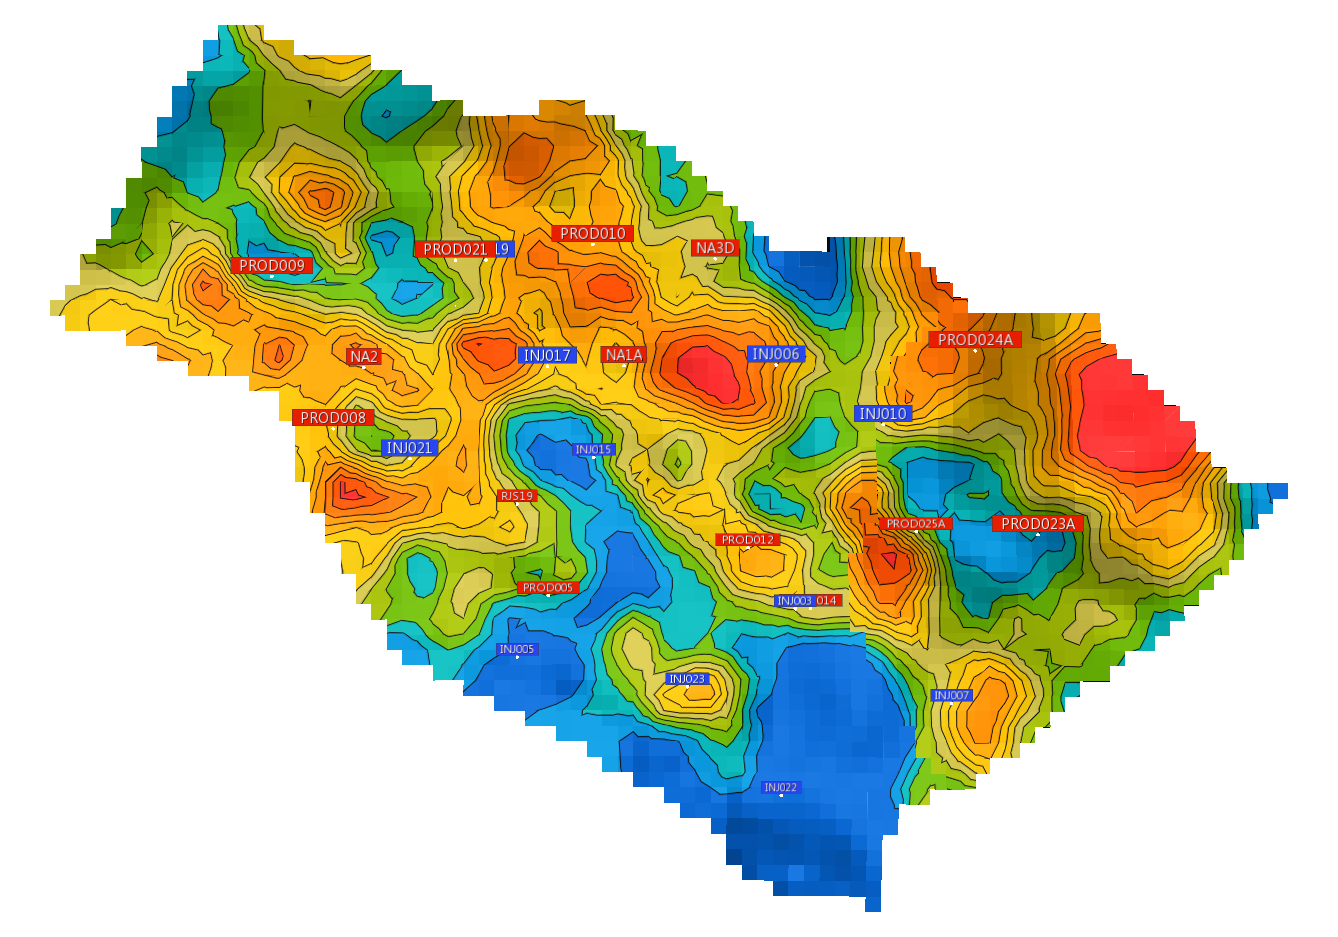
\includegraphics[width=0.85\columnwidth]{Geresim(0010).png}
  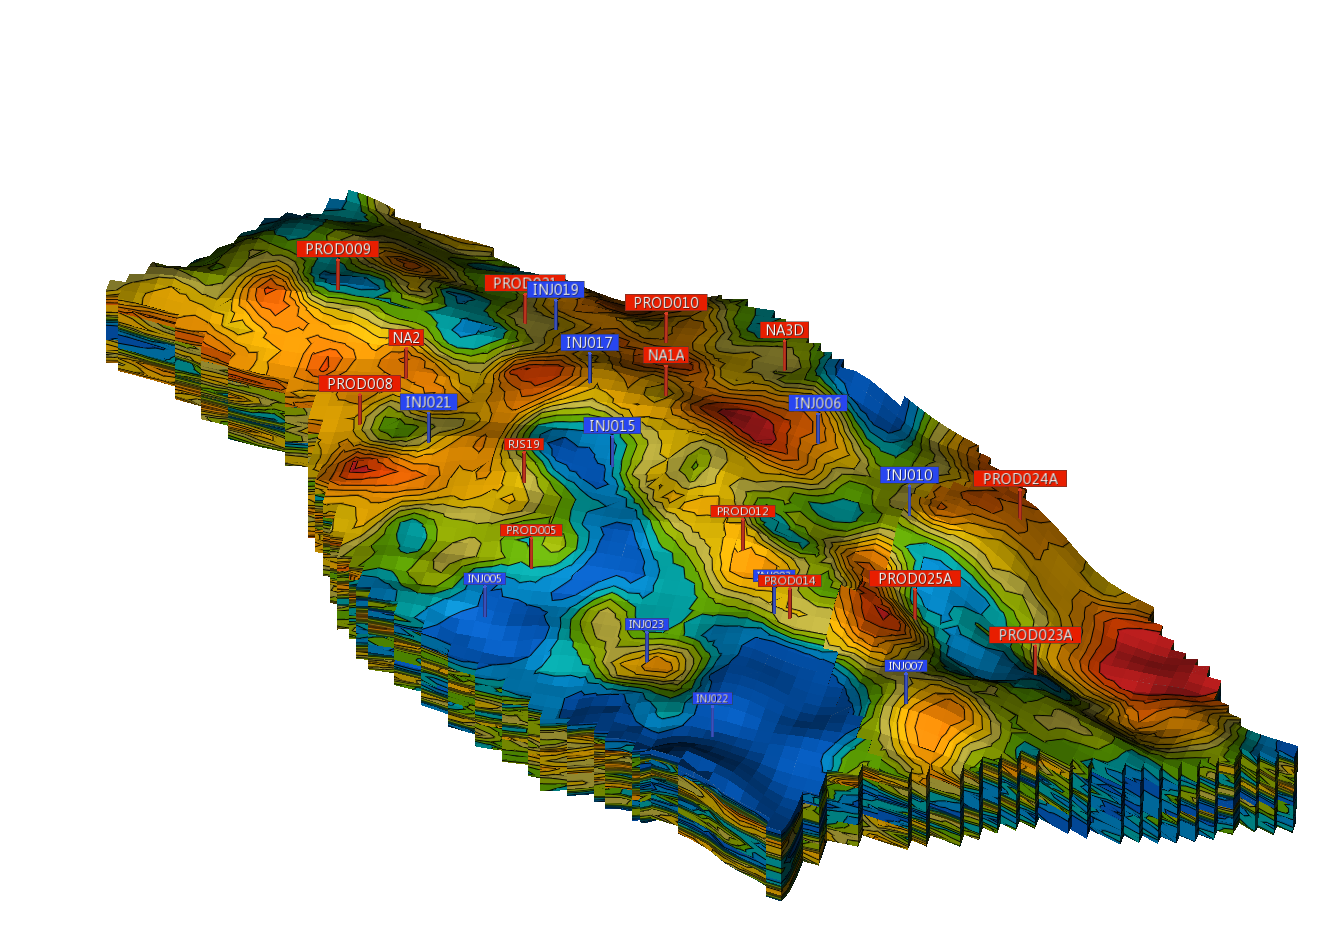
\includegraphics[width=0.85\columnwidth]{Geresim(0007).png}
  \caption{UNISIM-I-H geometry with the producer wells marked in red and injector wells marked in blue. The grid property shown is the field porosity.}
  \label{fig:unisim-sample}
\end{figure}

\begin{figure}[H]
  \centering
  \begin{subfigure}[b]{0.45\columnwidth}
    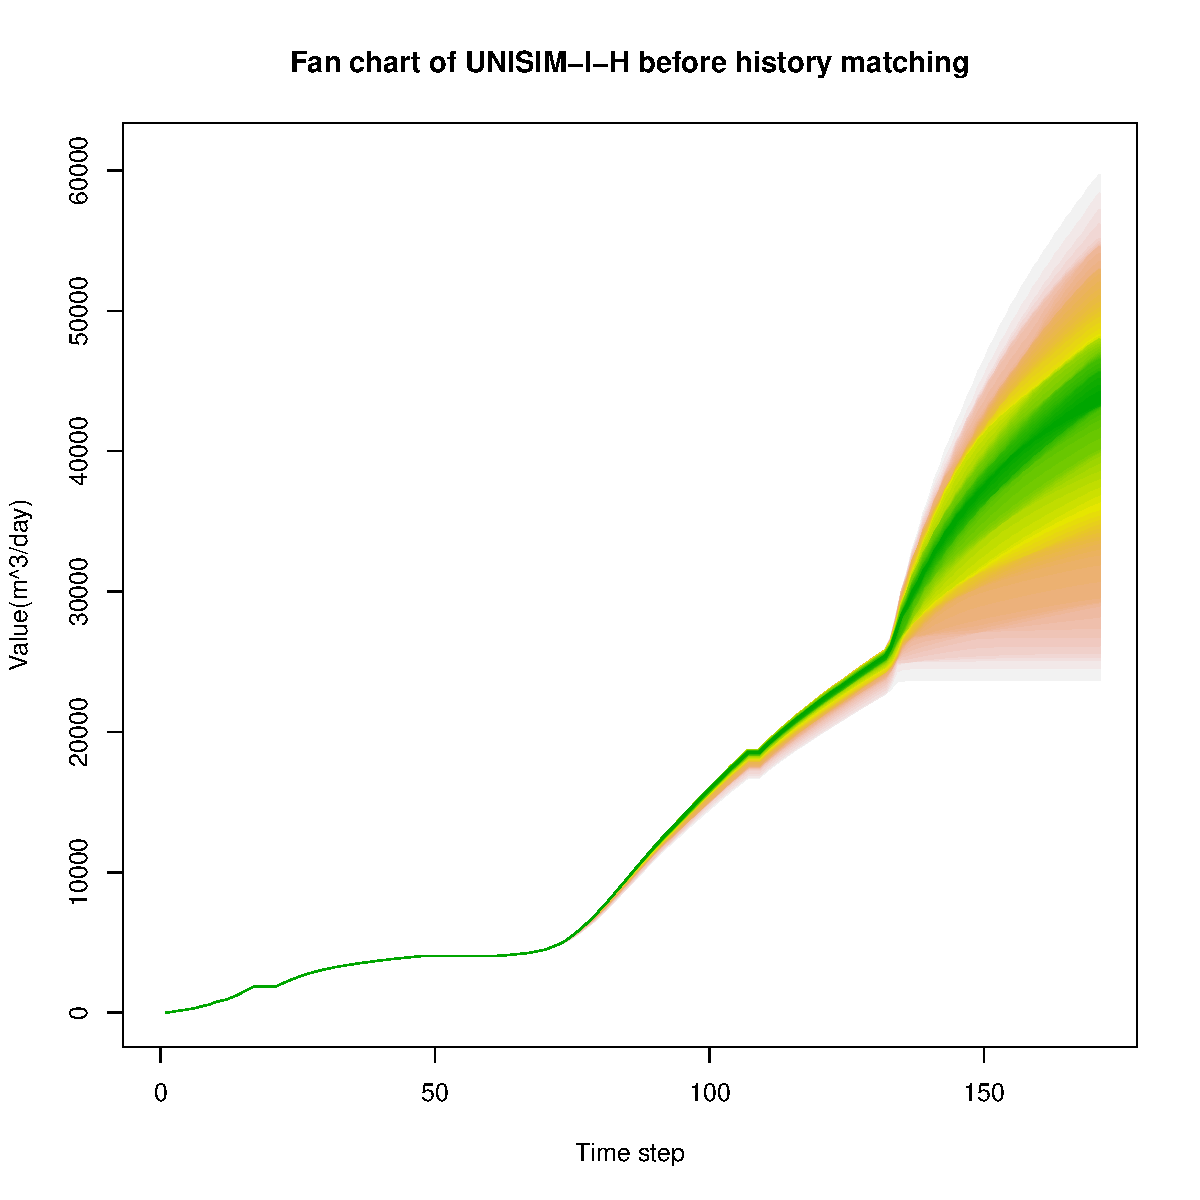
\includegraphics[width=\columnwidth]{fan-bef.pdf}
    \caption{}
    \label{fig:fan-bef}
  \end{subfigure}
  ~
  \begin{subfigure}[b]{0.45\columnwidth}
    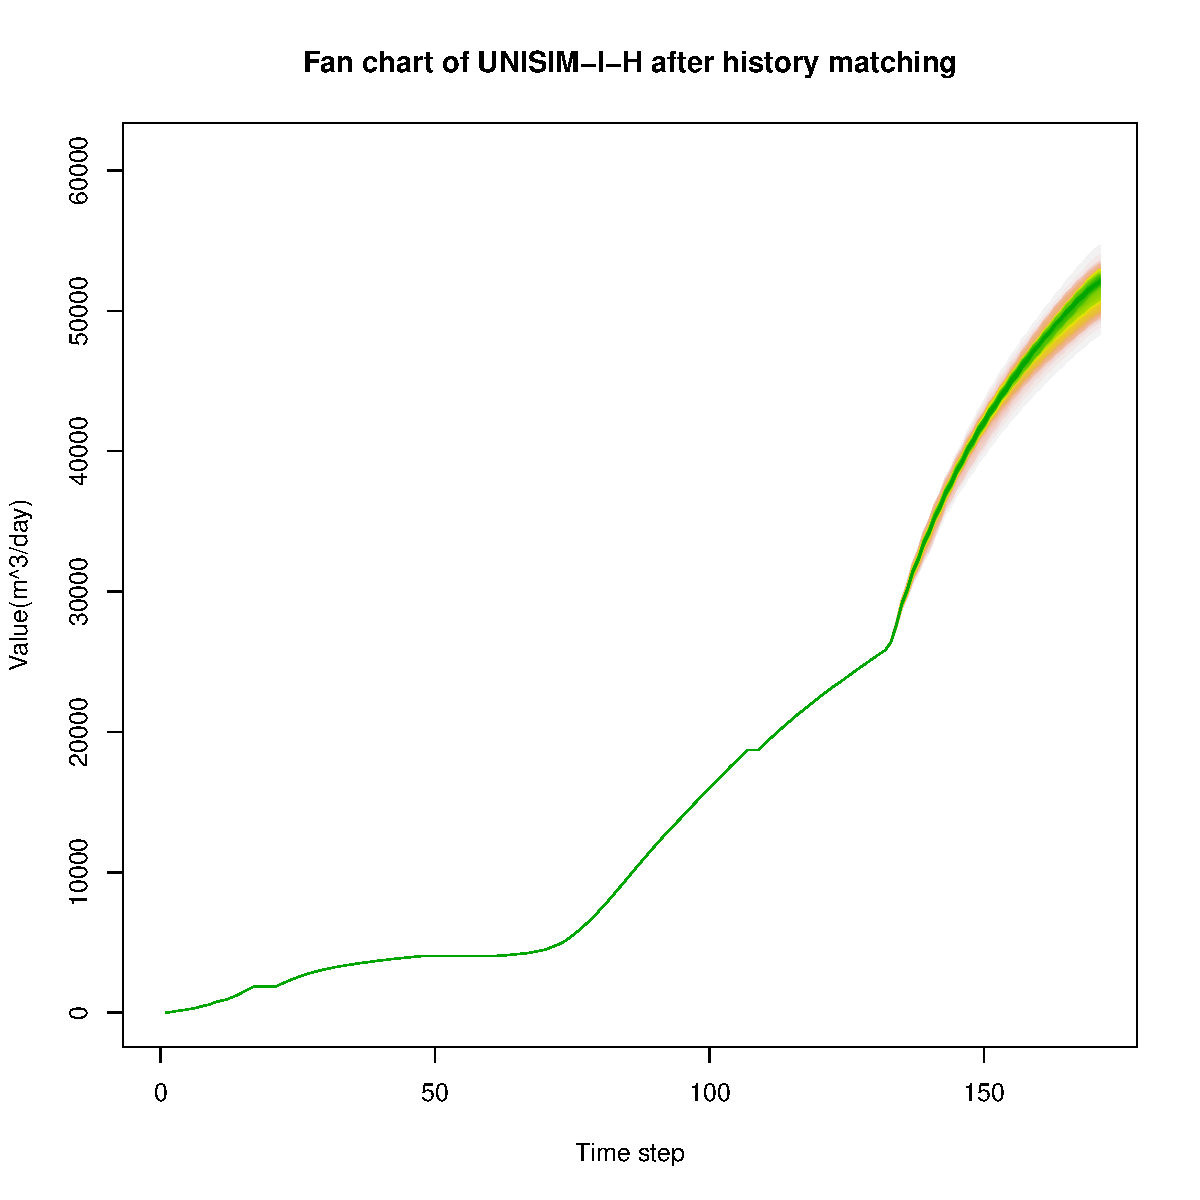
\includegraphics[width=\columnwidth]{fan-aft.pdf}
    \caption{}
    \label{fig:fan-aft}
  \end{subfigure}

  \caption{Cumulative oil production of the producer wells of the 200 UNISIM-I-H models before and after history matching.}
  \label{fig:fan-bef-aft}
\end{figure}

\subsection{Selection of Representative Models of Production Forecast}
\label{sec:percentile}
One of the key analysis tasks is the selection of statistically representative models of the forecast data. These are used as estimates for optimistic, median and pessimistic production. These models are used to estimate the performance of a production strategy if it were to be applied in the reservoir. They can be used to compare the performance of different strategies and their parameters can be used in new simulation runs to generate new, and more refined ensembles.

In several oil companies, the task of selecting such models is done manually by using spreadsheets \cite{selection-sarma:2013}. More sophisticated methods use variants of clustering algorithms to select the models automatically. The manual approach is time consuming and error prone, and any errors can lead to improper planning and formulation of inadequate strategies. The clustering approach is computationally faster, but it can select suboptimal models \cite{selection-sarma:2013}. Our hypothesis is that the rank chart can be a valuable tool to help in this process. By selecting a set of candidate models using our proposed score function or a manual approach using the charts described in Section \ref{sec:tools} linked together via a brushing \& linking approach, their adherence to the reference models can be visually inspected with the rank chart, and hopefully, a good set of representative models can be chosen from the candidates. The reference models chosen for our experiments are the P$_{10}$, P$_{50}$ and P$_{90}$ percentile curves calculated from the ensemble itself. These percentile curves are synthetic, and not part of the ensemble, and they represent optimistic, median and pessimistic production forecasts, respectively.

The process begins with the selection of the well properties to be processed and the calculation of the reference percentile curves. For the purposes of this test, only the group of producer wells was used, meaning that of the 25 wells in each simulation, only data from 14 were used. Since the user of a system in this context wants to maximize the oil production of a field, our analysis focused on the cumulative oil production (NP) of the producer wells group. Figure \ref{fig:np-chart} shows the overlaid line charts of the forecasts of 200 ensemble curves in gray, and the calculated percentiles.

\begin{figure}[H]
  \centering
  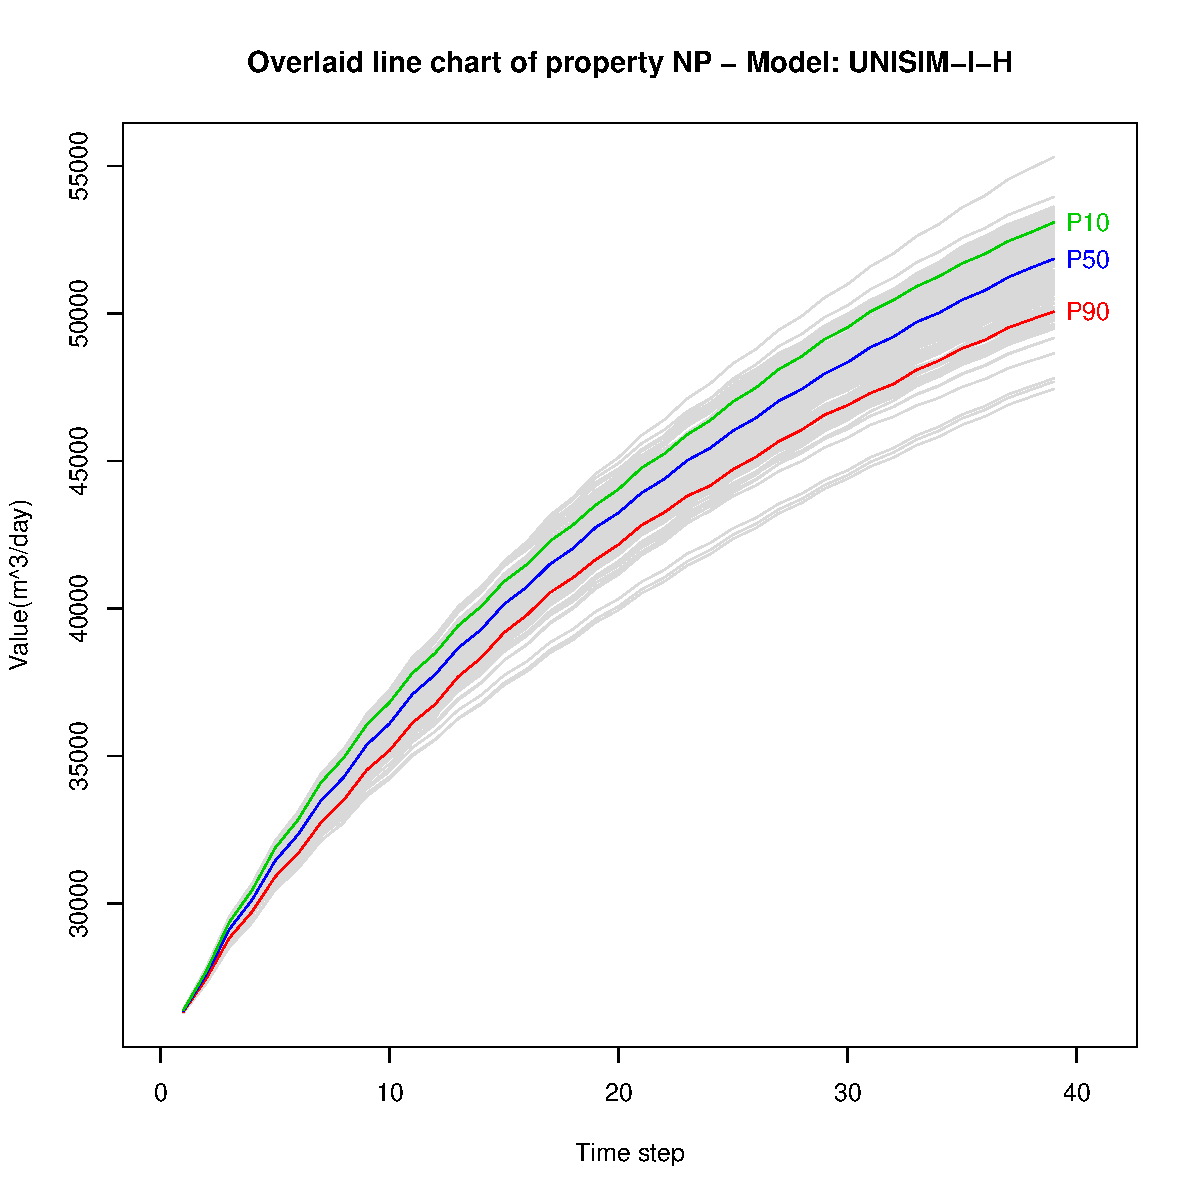
\includegraphics[width=\columnwidth]{np-spag.pdf}
  \caption{Overlaid line charts of the cumulative oil production for the producer wells of our ensemble. The percentile curves P$_{10}$, P$_{50}$ and P$_{90}$ are marked in green, blue and red respectively.}
  \label{fig:np-chart}
\end{figure}

To apply the algorithm described in section \ref{sec:obj_func}, we must define a weight function for the simulation time steps. For this kind of data, we have chosen an arc-tangent based function, where the time step index is used as argument: $w(t) = arctan(t)$. This function enables us to assign a higher weight to time steps towards the end of the simulation, where the curves have a higher spread. Since the property chosen was the cumulative oil production, the curves have a very small spread in the beginning of the forecasted simulation time and a large spread nearing the end of the simulation, as shown in Figure \ref{fig:np-chart}. This way, curves with better ranking towards the end of the simulation will be assigned a higher score, compensanting for the higher curve spread.

The first set of candidates was selected automatically by the scoring algorithm described in Section \ref{sec:obj_func}. We have selected the first 5 entities with the highest scores as possible candidates for each percentile. A side-by-side view of the rank and fan charts of the score selected curves is shown in Figure \ref{fig:rank-fan-score}. For all fan charts, the percentiles P$_{10}$, P$_{50}$ and P$_{90}$ are marked in green, blue and red respectively; the models selected by each approach are marked in black.

\begin{figure}[H]
  \centering
  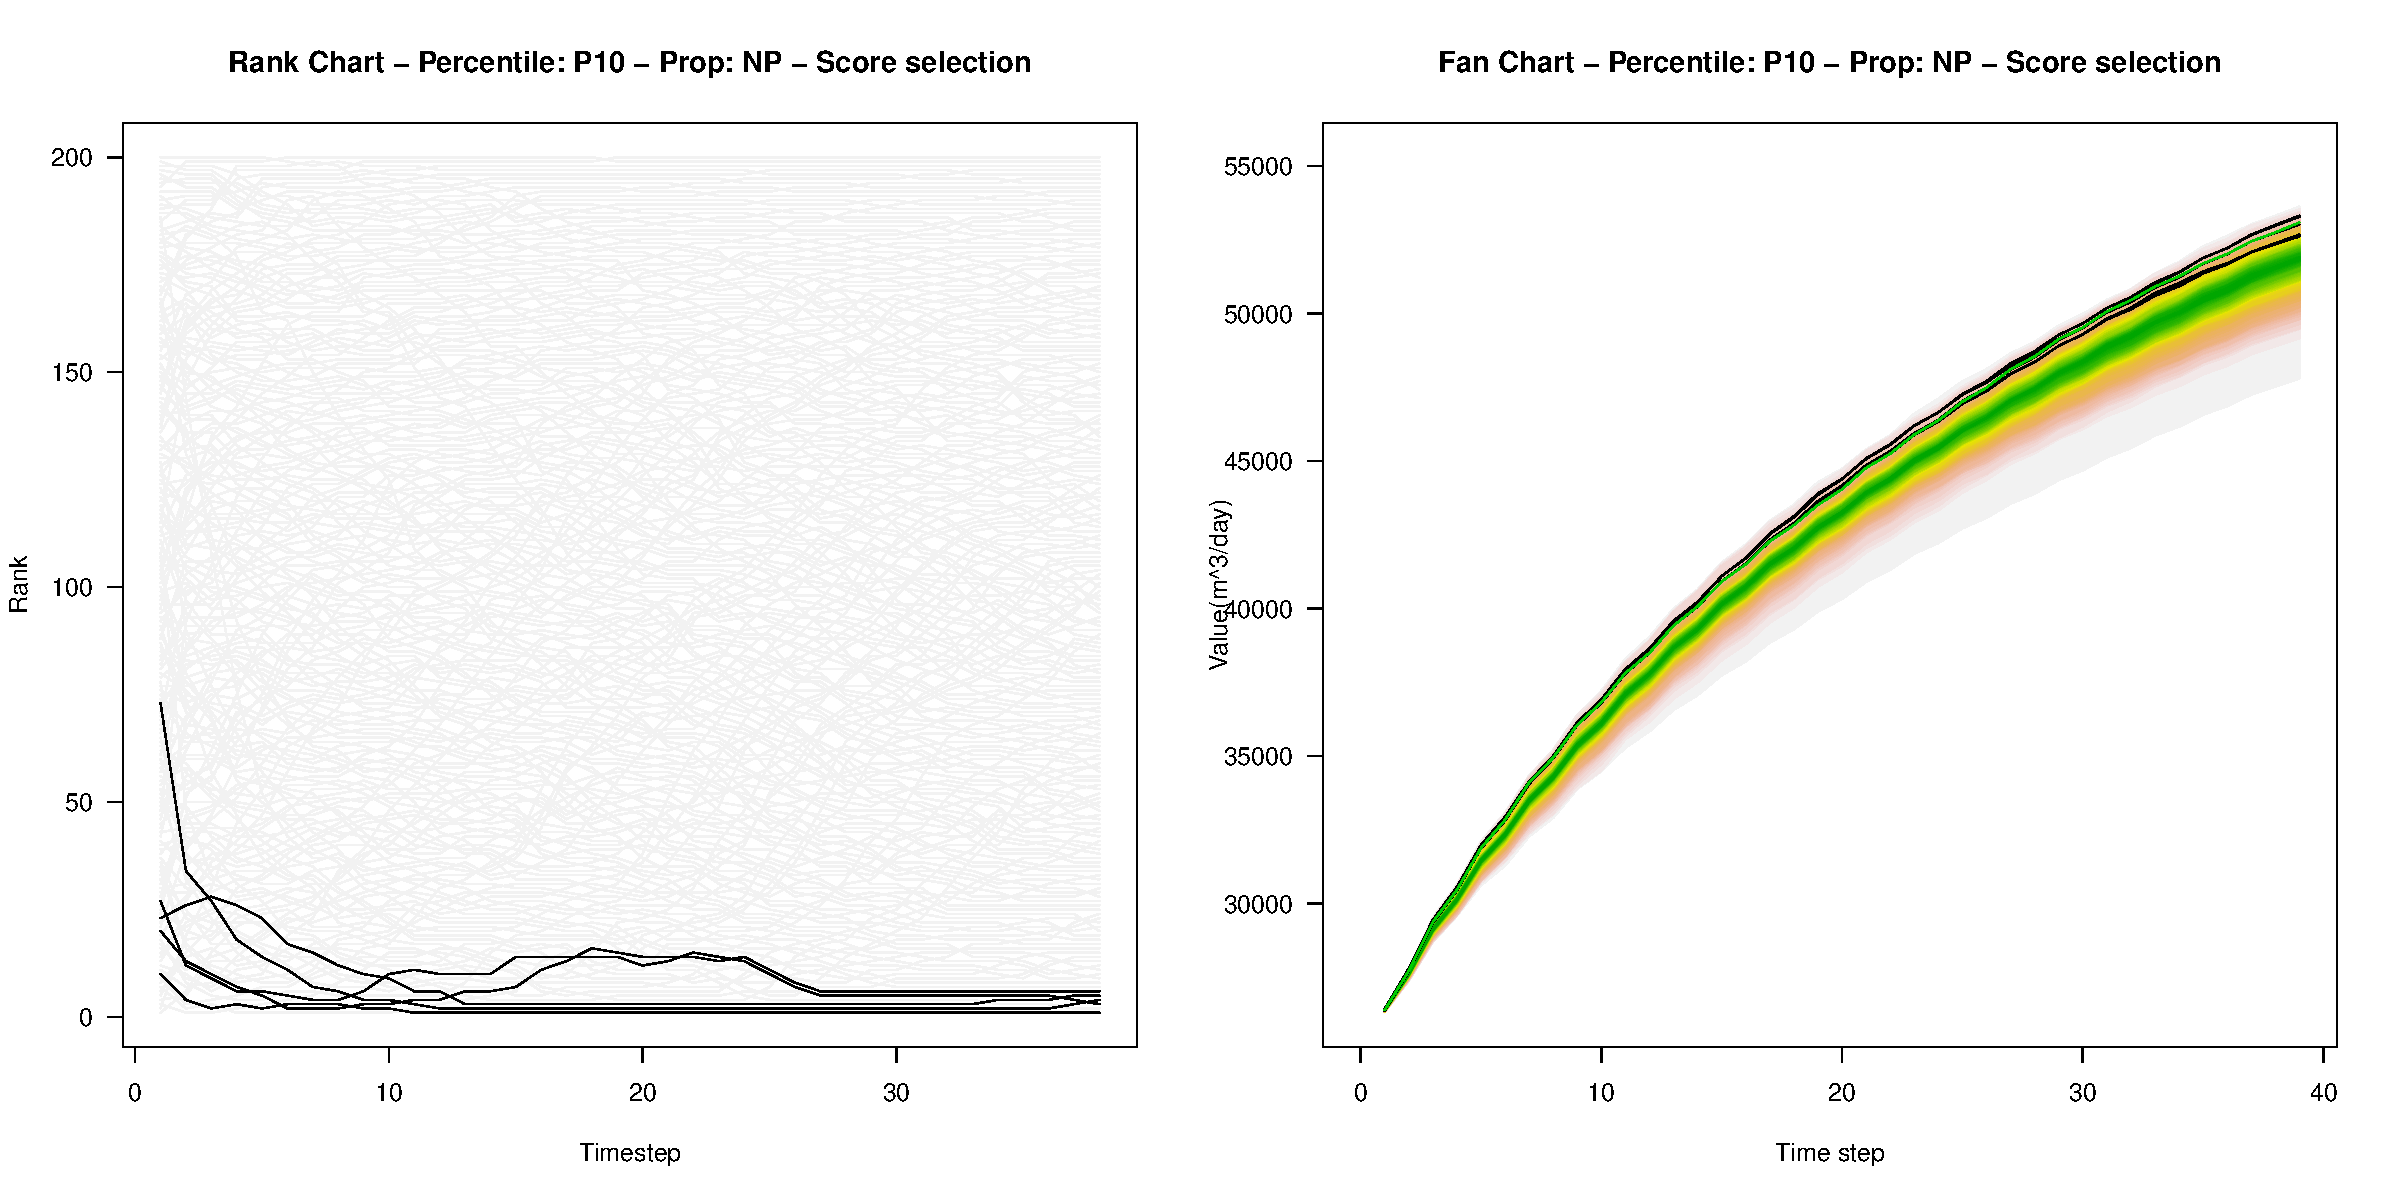
\includegraphics[width=0.78\columnwidth]{rank-fan-score-p10.pdf}
  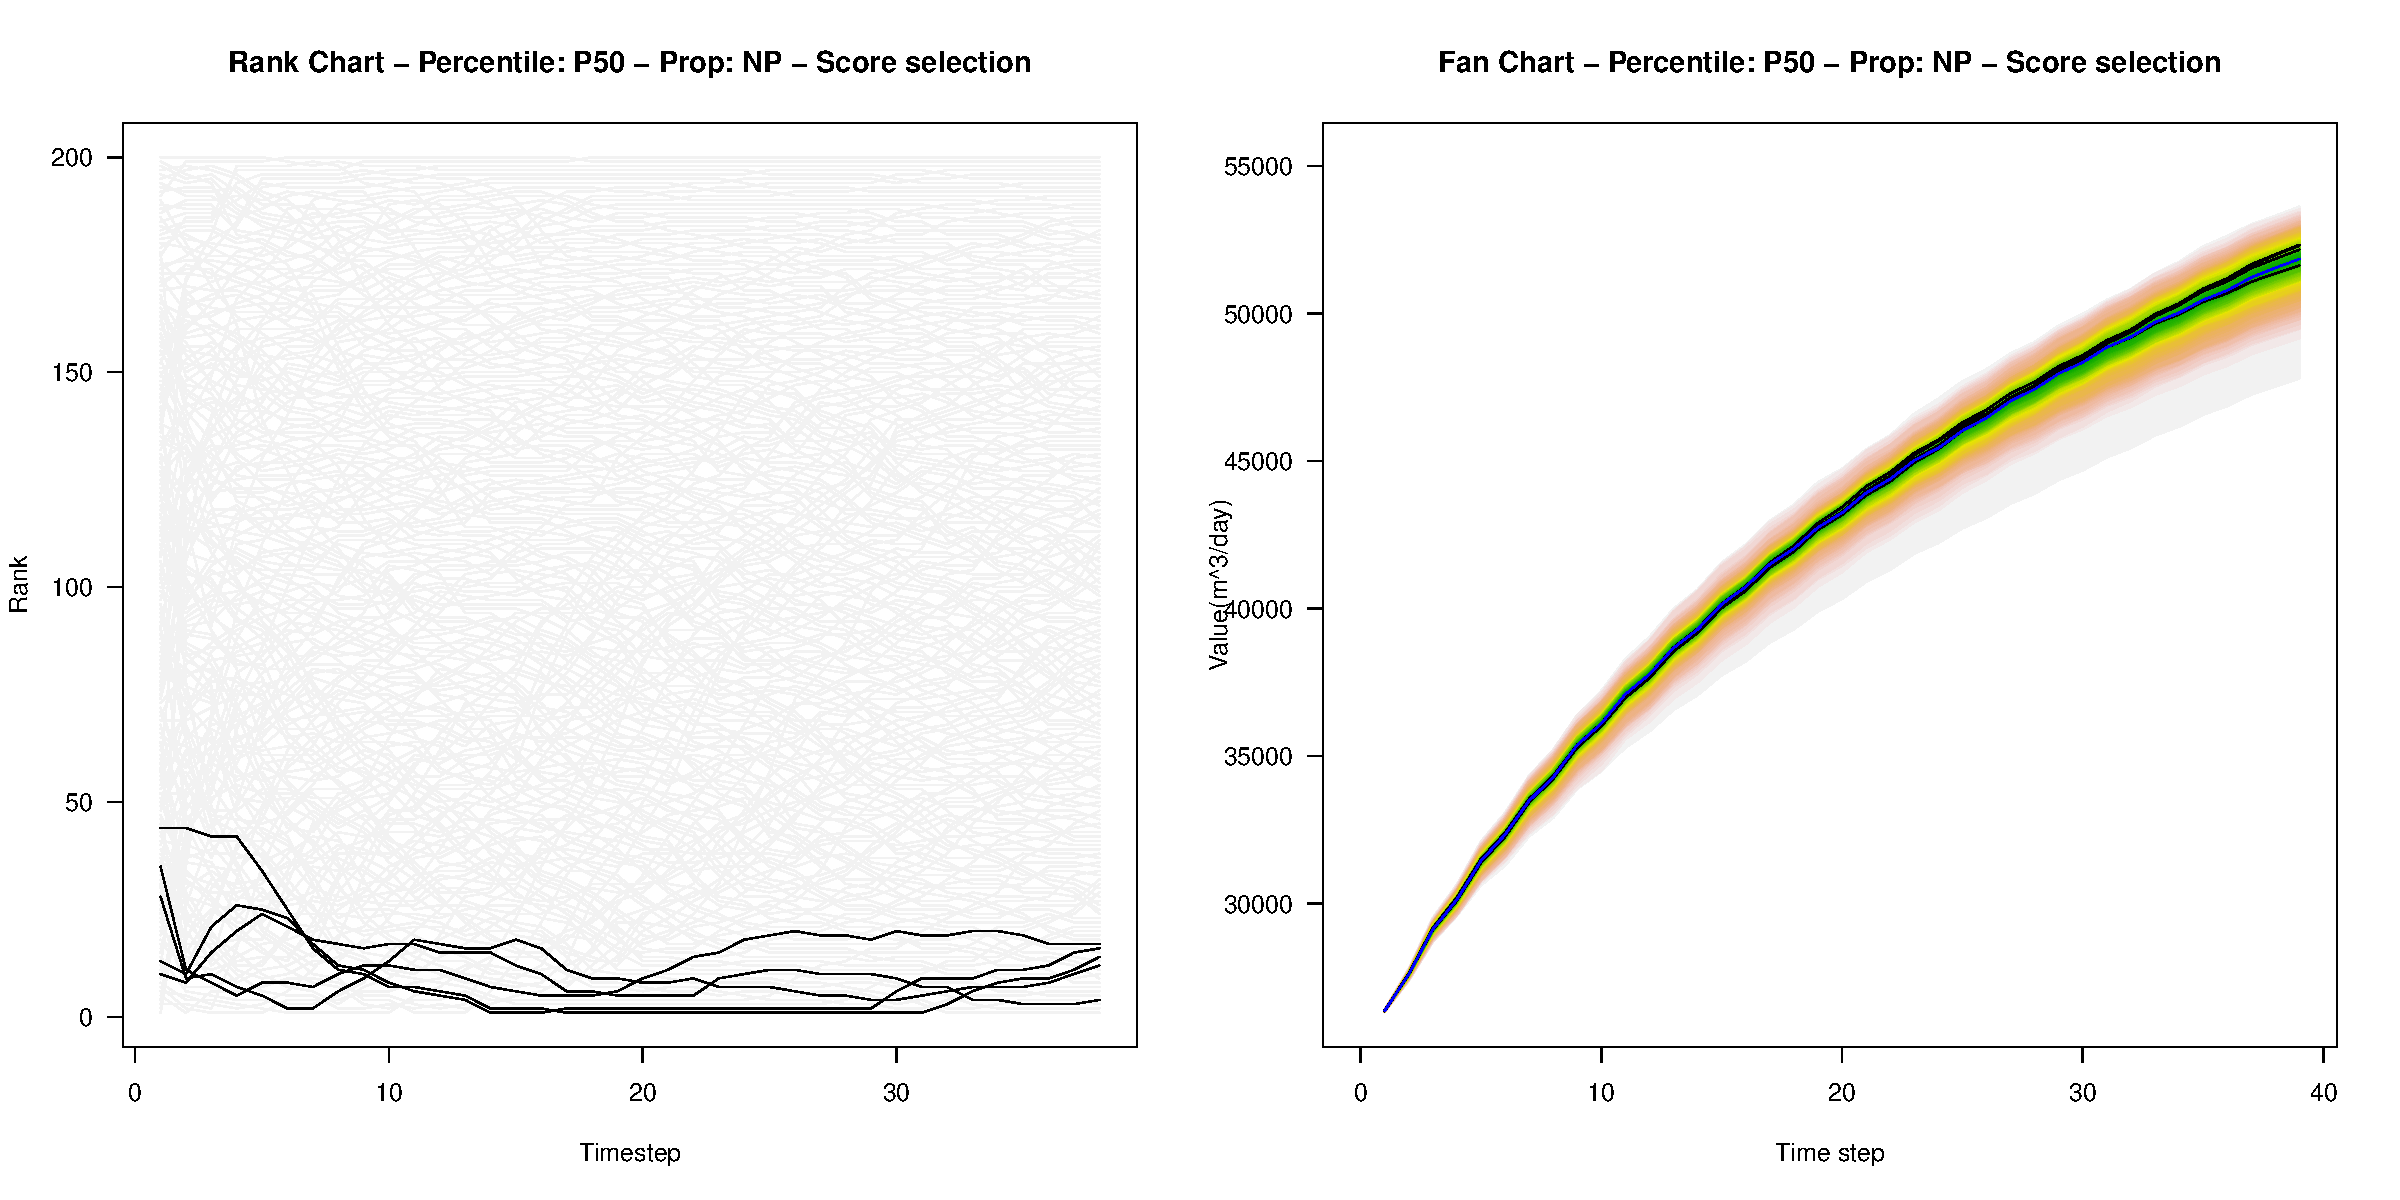
\includegraphics[width=0.78\columnwidth]{rank-fan-score-p50.pdf}
  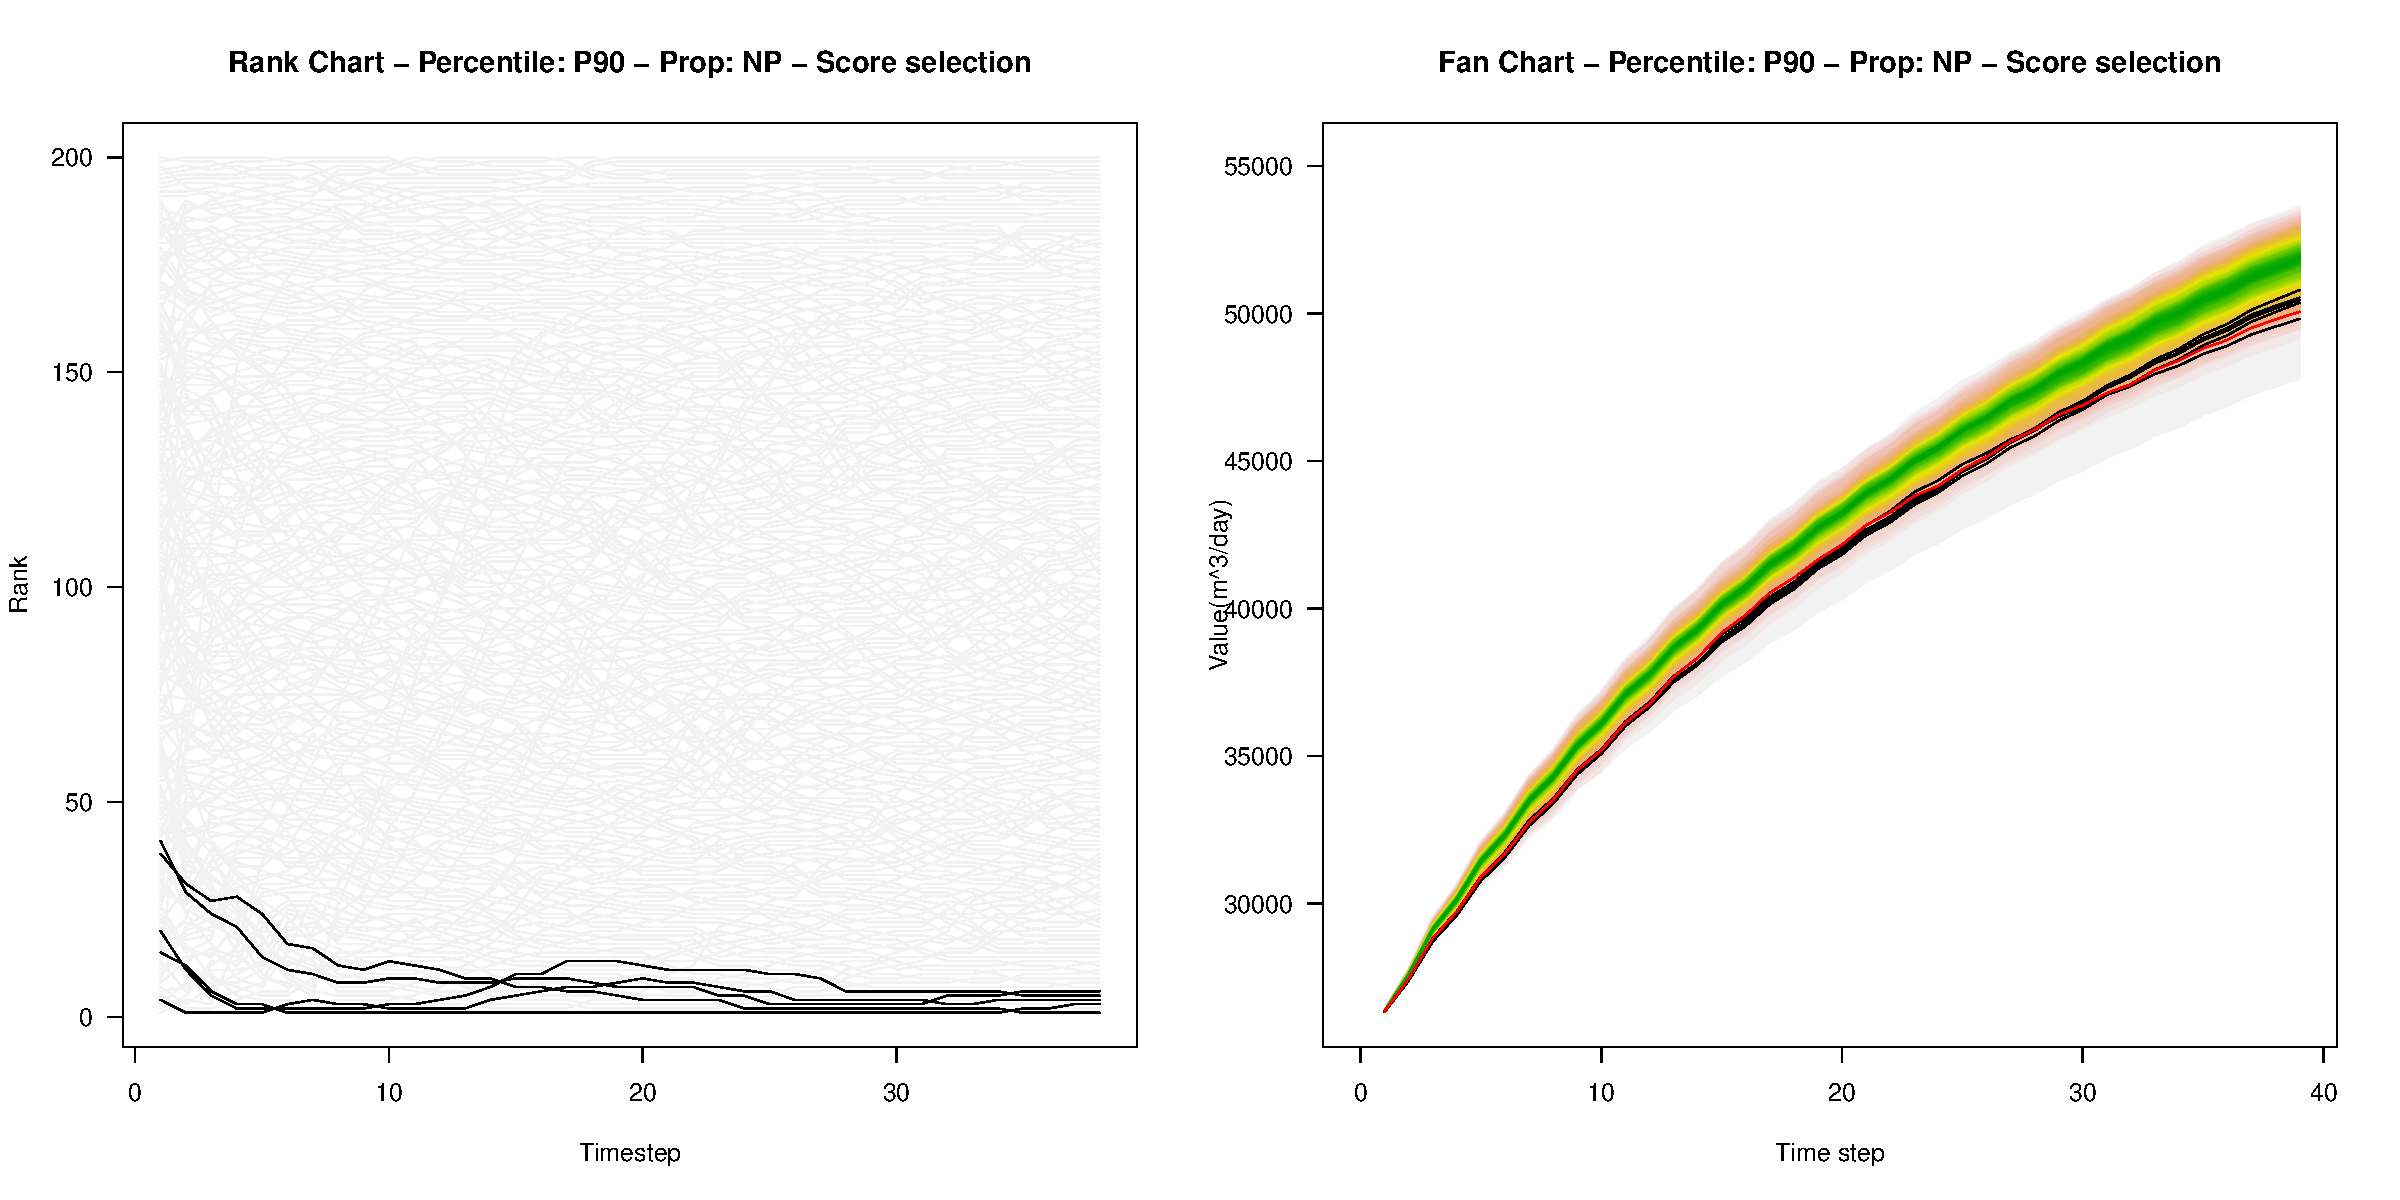
\includegraphics[width=0.78\columnwidth]{rank-fan-score-p90.pdf}
  \caption{Side-by-side rank and fan charts with the score selected curves highlighted. The selected models are UNISIM\_66, UNISIM\_156, UNISIM\_167, UNISIM\_87 and UNISIM\_54 for P$_{10}$; UNISIM\_71, UNISIM\_30, UNISIM\_174, UNISIM\_45 and UNISIM\_135 for P$_{50}$; and UNISIM\_147, UNISIM\_58, UNISIM\_53, UNISIM\_186 and UNISIM\_111 for P$_{90}$.}
  \label{fig:rank-fan-score}
\end{figure}

The rank charts in Figure \ref{fig:rank-fan-score} show that the curves have a relatively poor adherence to the reference curve in the first time steps, but since the curves have a low spread, this difference is barely noticeable as shown in the equivalent fan charts. However, as the curves approach the end of the simulation a higher weight is assigned to them in order to ensure that the curves with a better adherence will score higher, thus resulting in a better ranking.

A second set of curves was selected by using the brushing \& linking framework. These candidates are manually brushed using a Scenario/Distance chart, shown in Figure \ref{fig:scen-brush}, and are visually compared to the first set by using the tools described in Section \ref{sec:tools}. Figure \ref{fig:rank-fan-brush} shows the side by side view of the rank and fan charts of the second set curves. In addition, a comparative MDS projection is calculated using the whole time range of forecasted data of the cumulative oil property. Figure \ref{fig:mds-plots} shows the projections of candidates from the first and second sets. For all MDS projections, the percentiles P$_{10}$, P$_{50}$ and P$_{90}$ are marked in the same way as the fan charts, however, the selected models are marked in orange in the MDS scatter charts.

\begin{figure}[H]
  \centering
  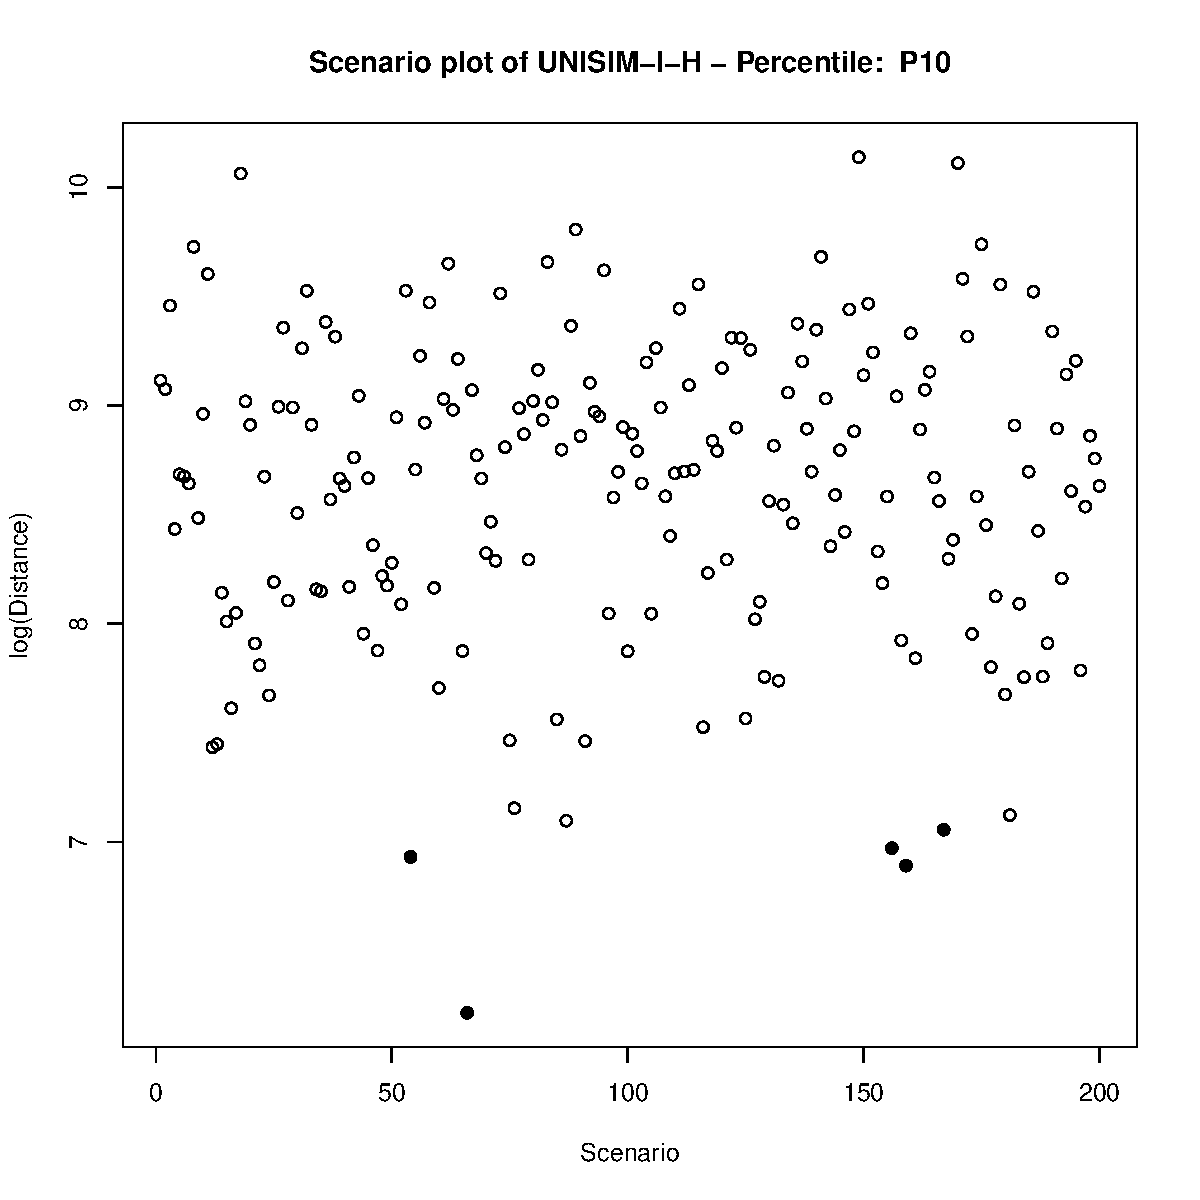
\includegraphics[width=0.45\columnwidth]{scen-NP-p10-log.pdf}
  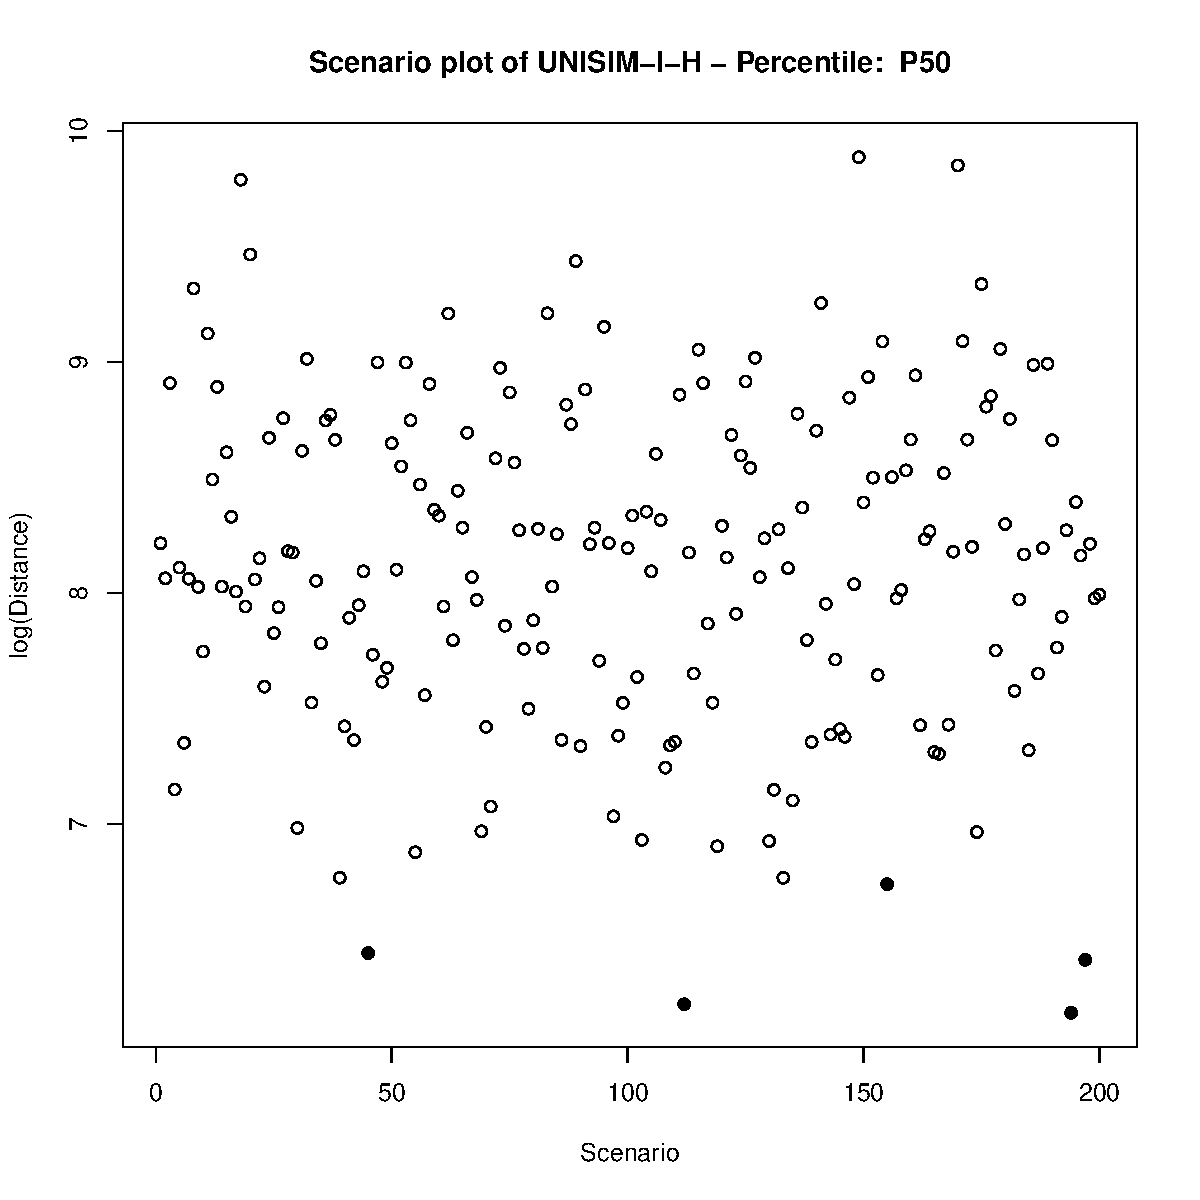
\includegraphics[width=0.45\columnwidth]{scen-NP-p50-log.pdf}
  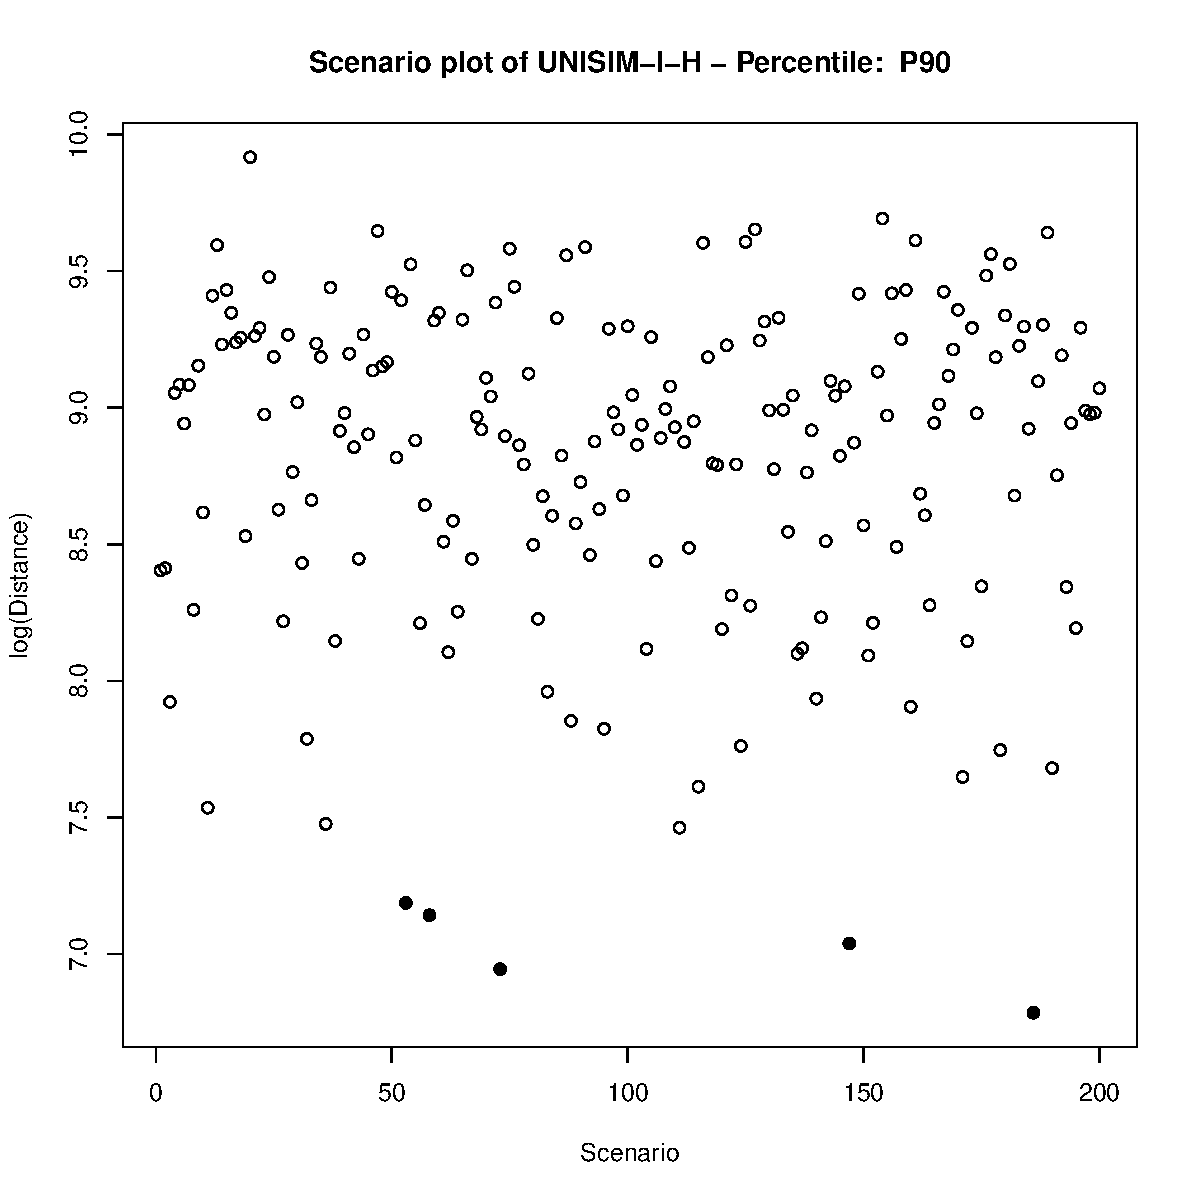
\includegraphics[width=0.45\columnwidth]{scen-NP-p90-log.pdf}
  \caption{Scenario charts of the manually selected curves. The $y$ axis is in logarithmic scale to ease the interpretation.}
  \label{fig:scen-brush}
\end{figure}

\begin{figure}[H]
  \centering
  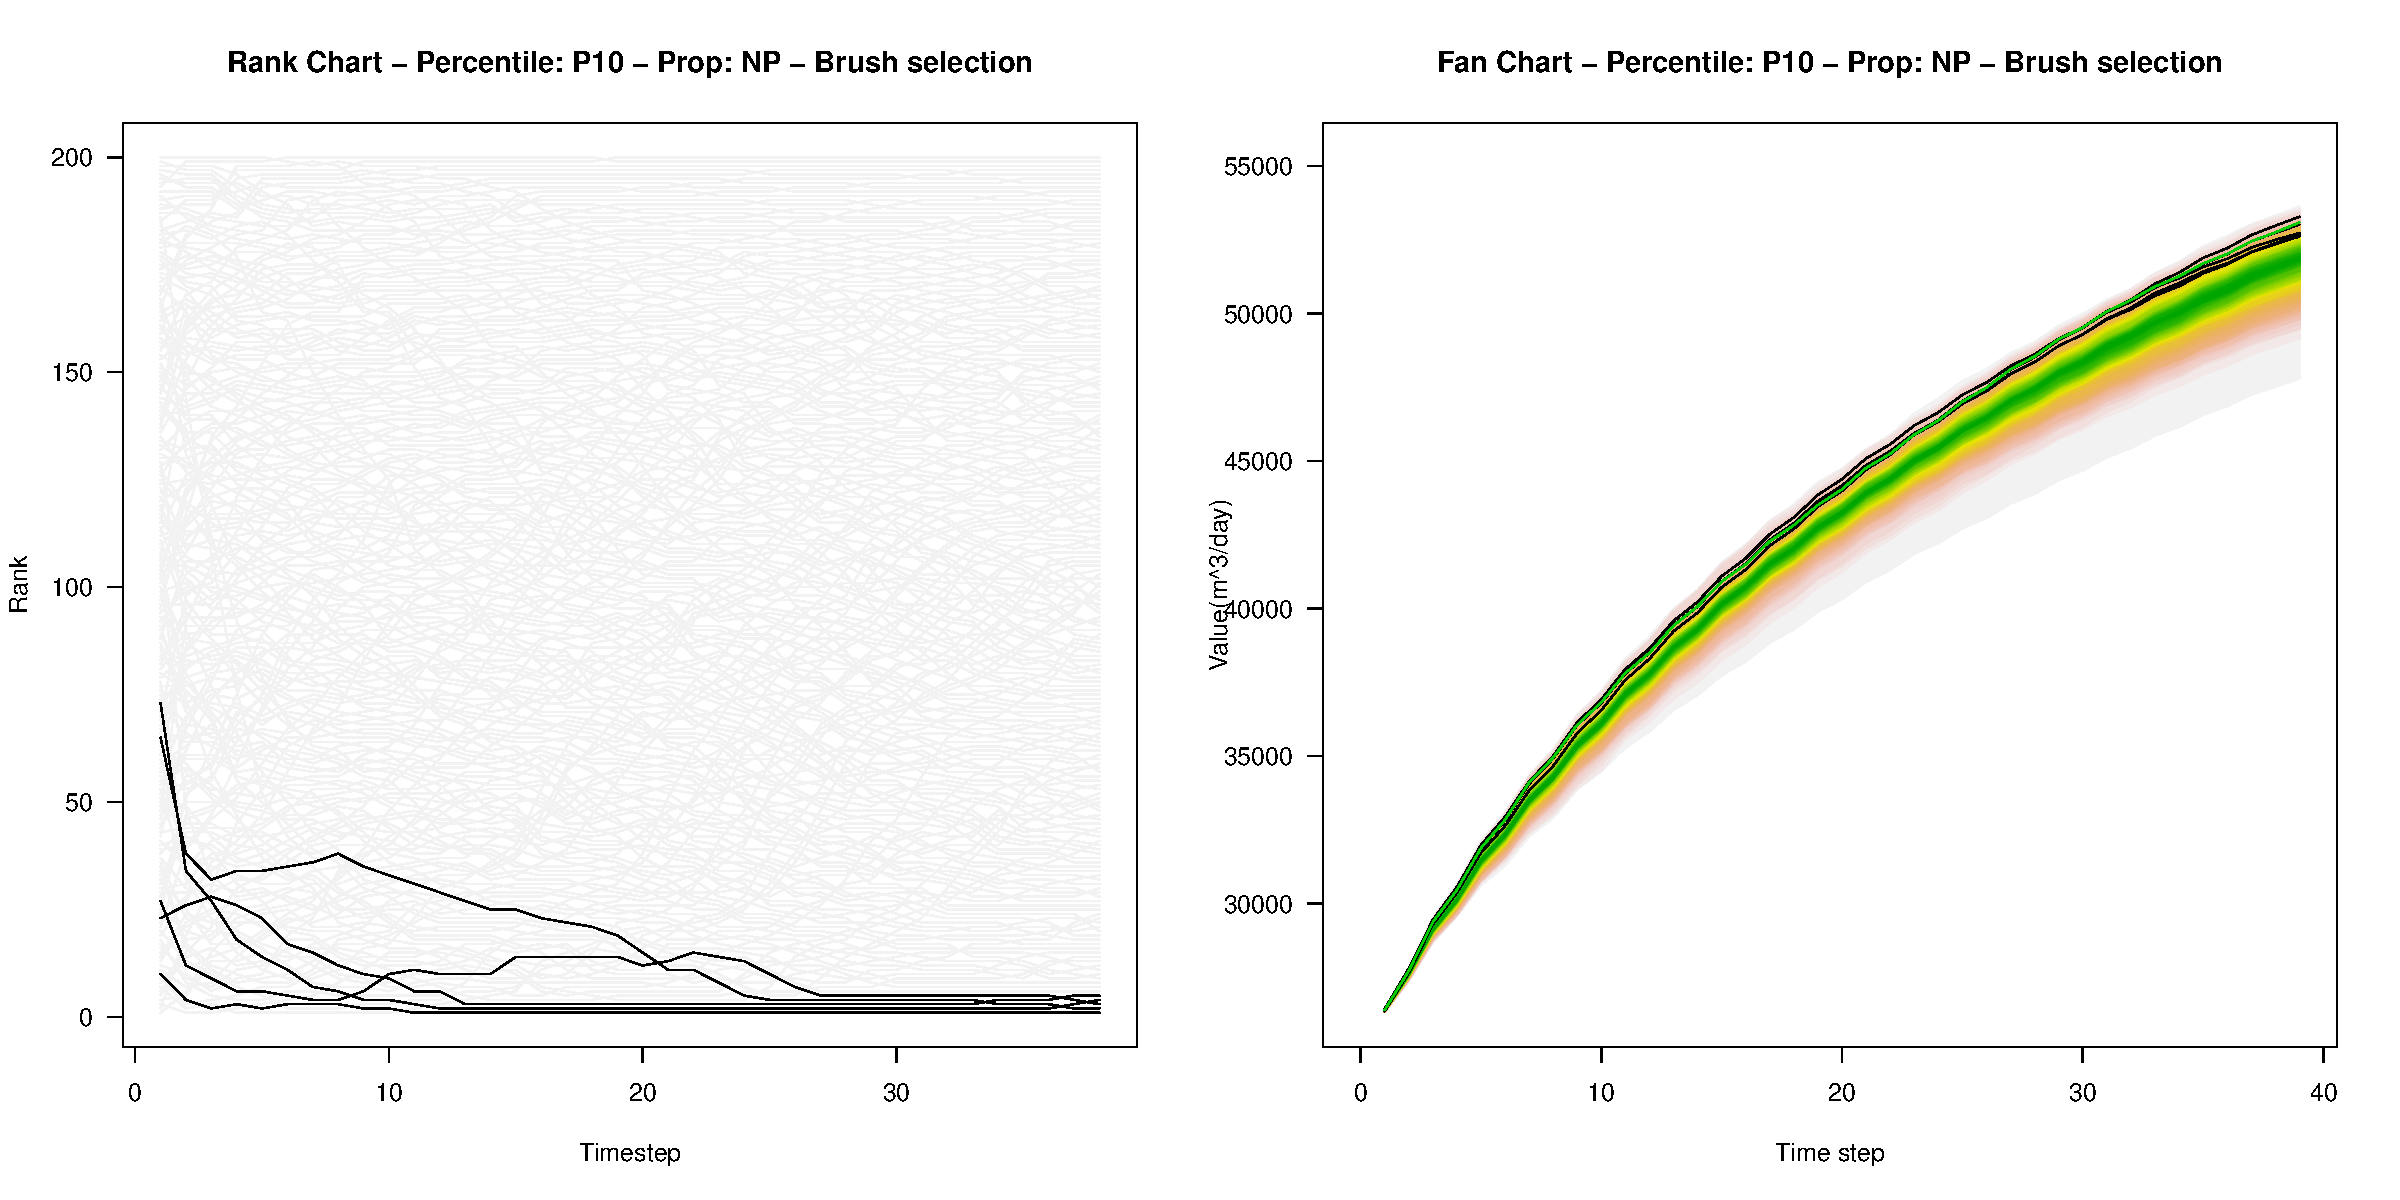
\includegraphics[width=0.8\columnwidth]{rank-fan-brush-p10.pdf}
  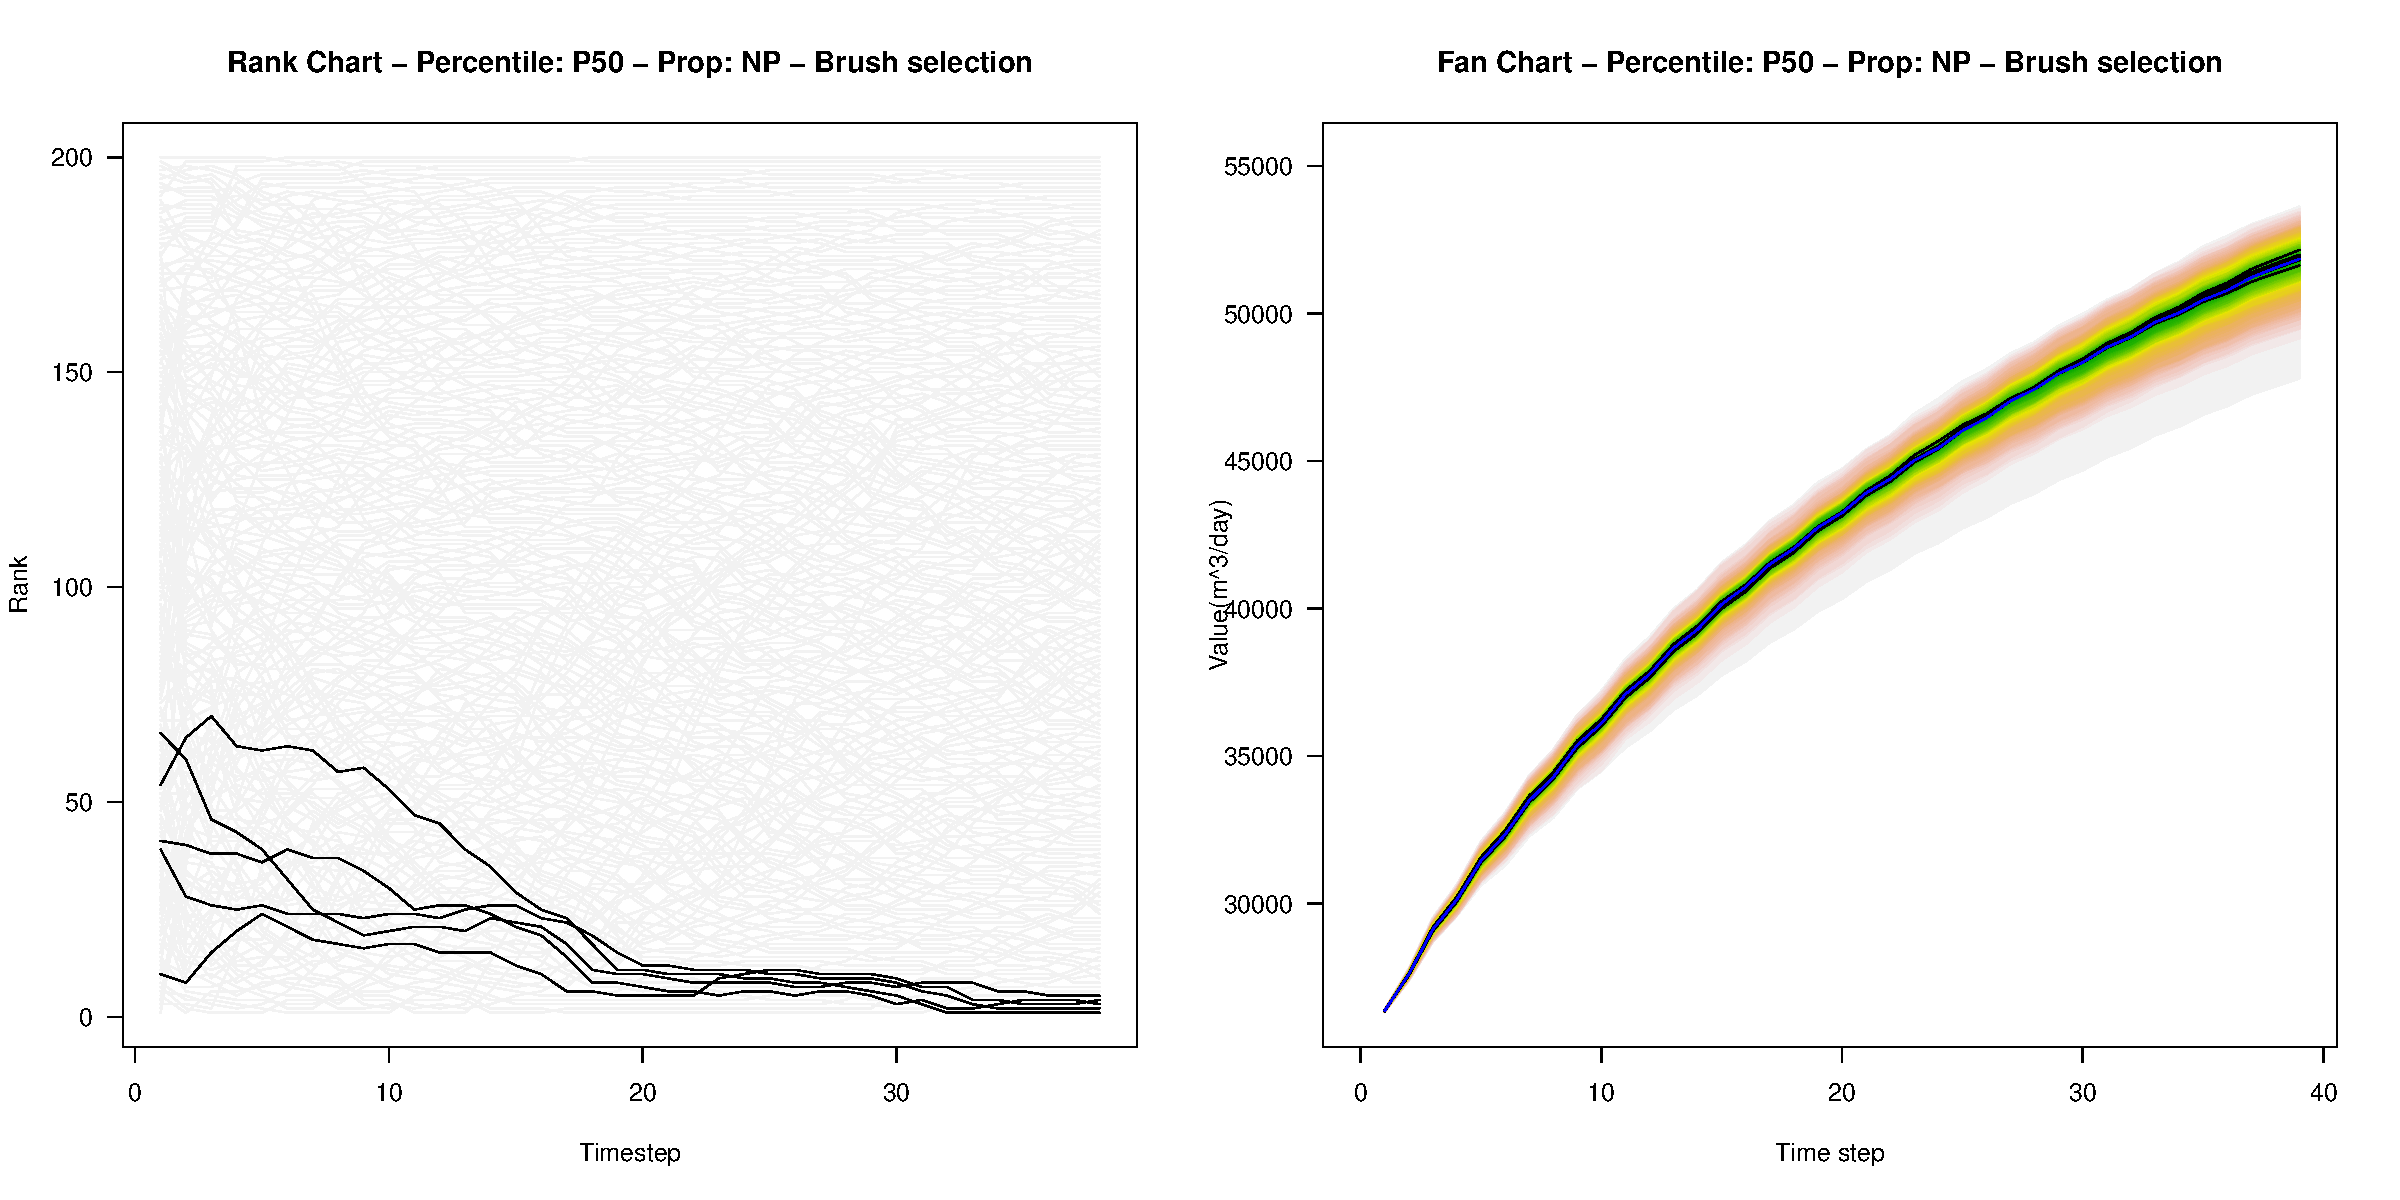
\includegraphics[width=0.8\columnwidth]{rank-fan-brush-p50.pdf}
  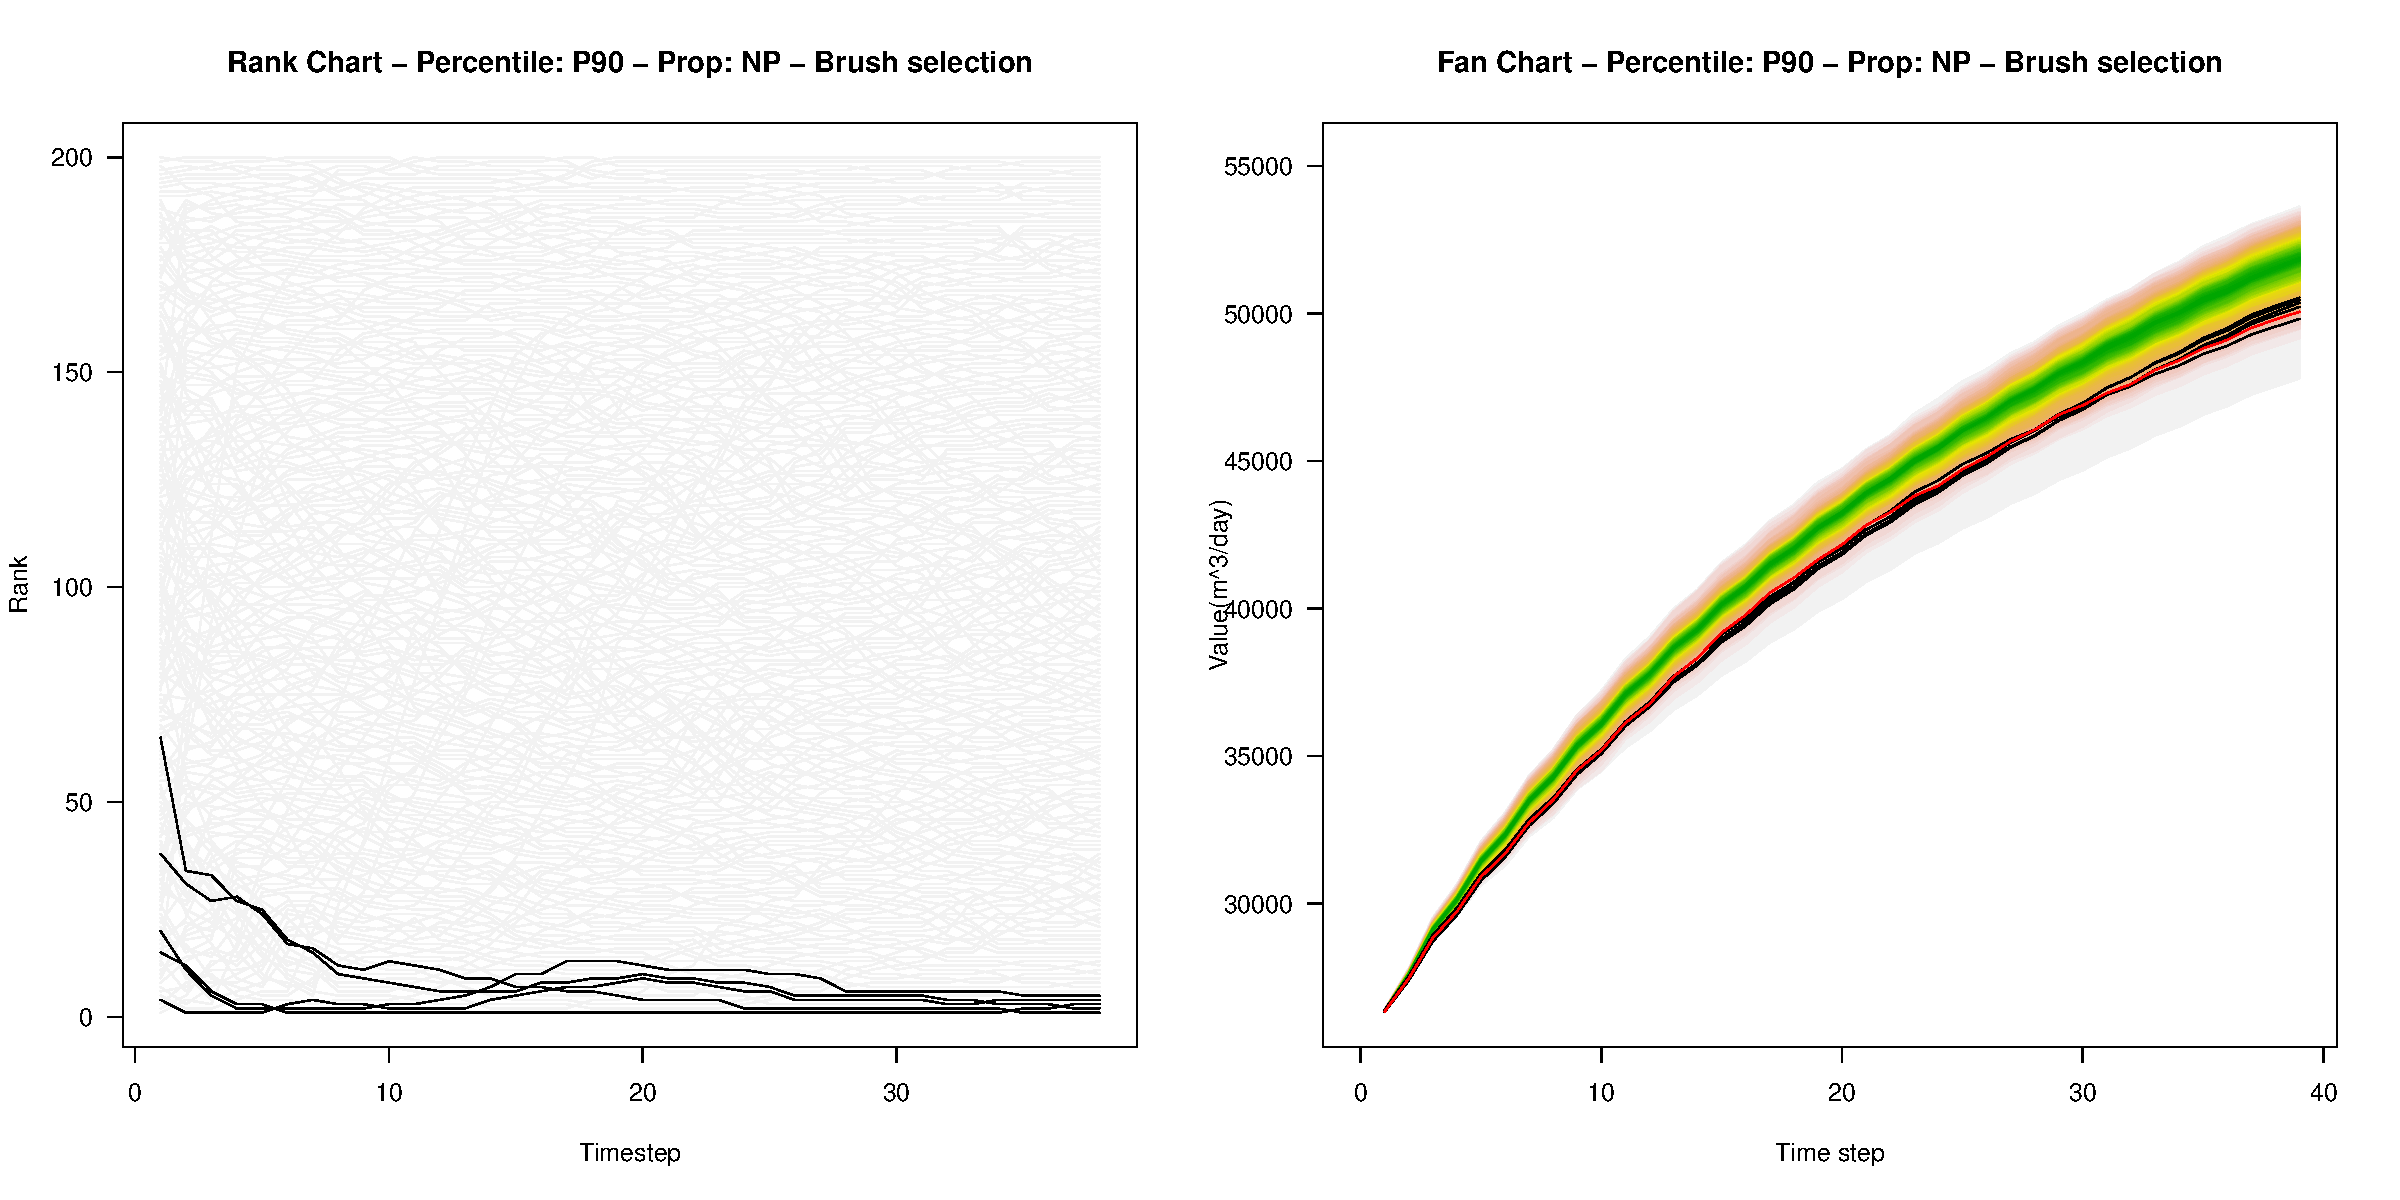
\includegraphics[width=0.8\columnwidth]{rank-fan-brush-p90.pdf}
  \caption{Side-by-side rank and fan charts with the manually selected curves highlighted. The selected models are UNISIM\_66, UNISIM\_159, UNISIM\_54, UNISIM\_156 and UNISIM\_167 for P$_{10}$; UNISIM\_194, UNISIM\_112, UNISIM\_197, UNISIM\_45 and UNISIM\_155 for P$_{50}$; and UNISIM\_186, UNISIM\_73, UNISIM\_147, UNISIM\_58 and UNISIM\_53 for P$_{90}$.}
  \label{fig:rank-fan-brush}
\end{figure}

\begin{figure}[H]
  \centering
  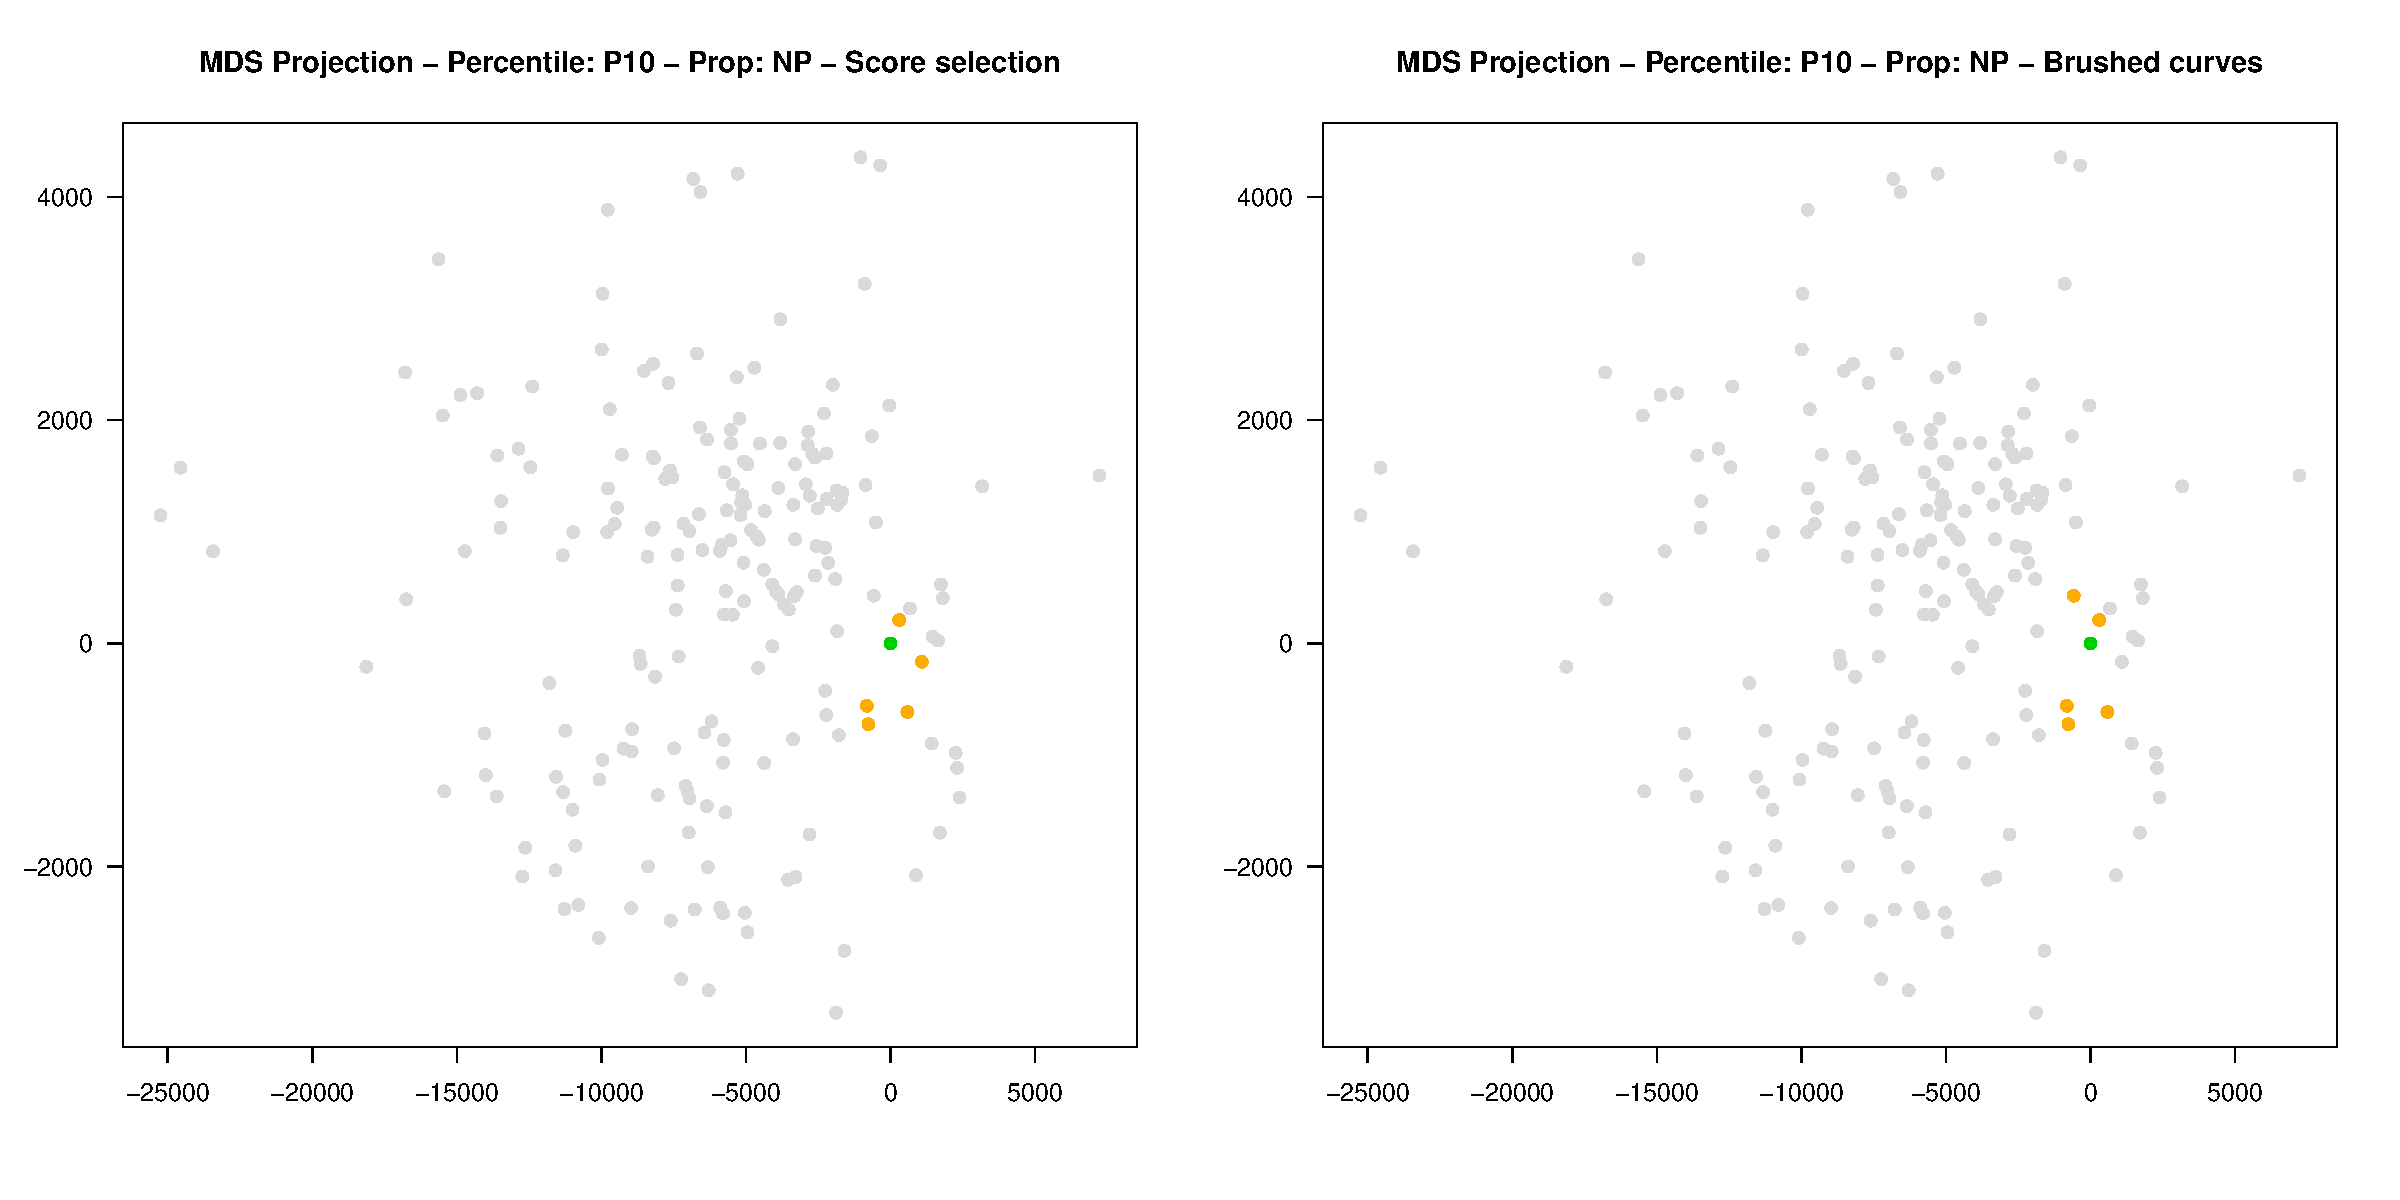
\includegraphics[width=0.88\columnwidth]{figures/mds-brush-score-p10.pdf}
  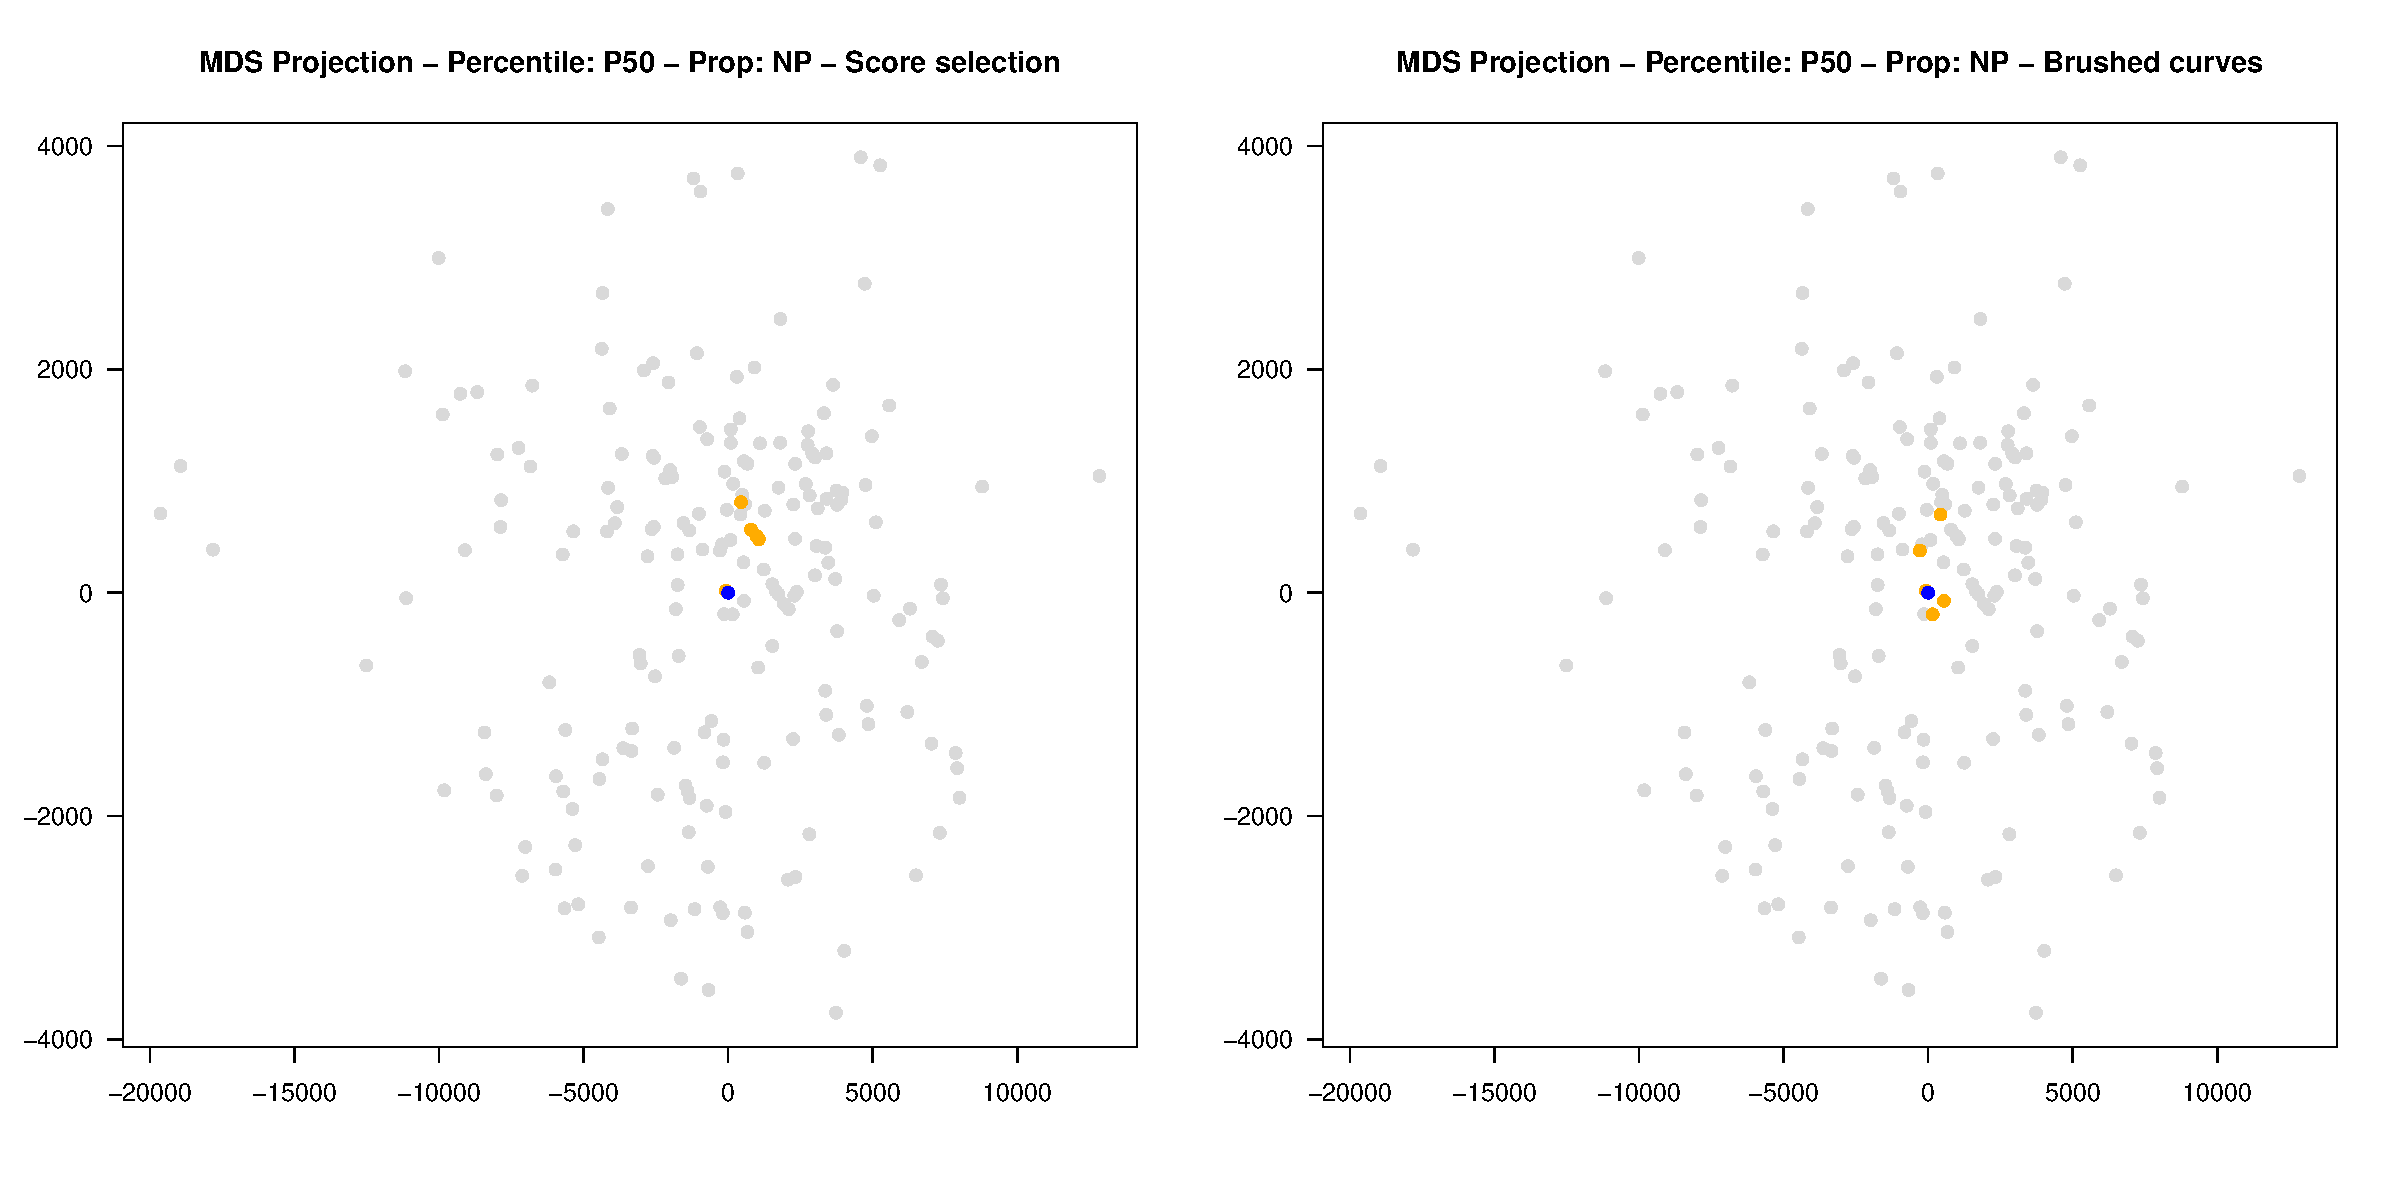
\includegraphics[width=0.88\columnwidth]{figures/mds-brush-score-p50.pdf}
  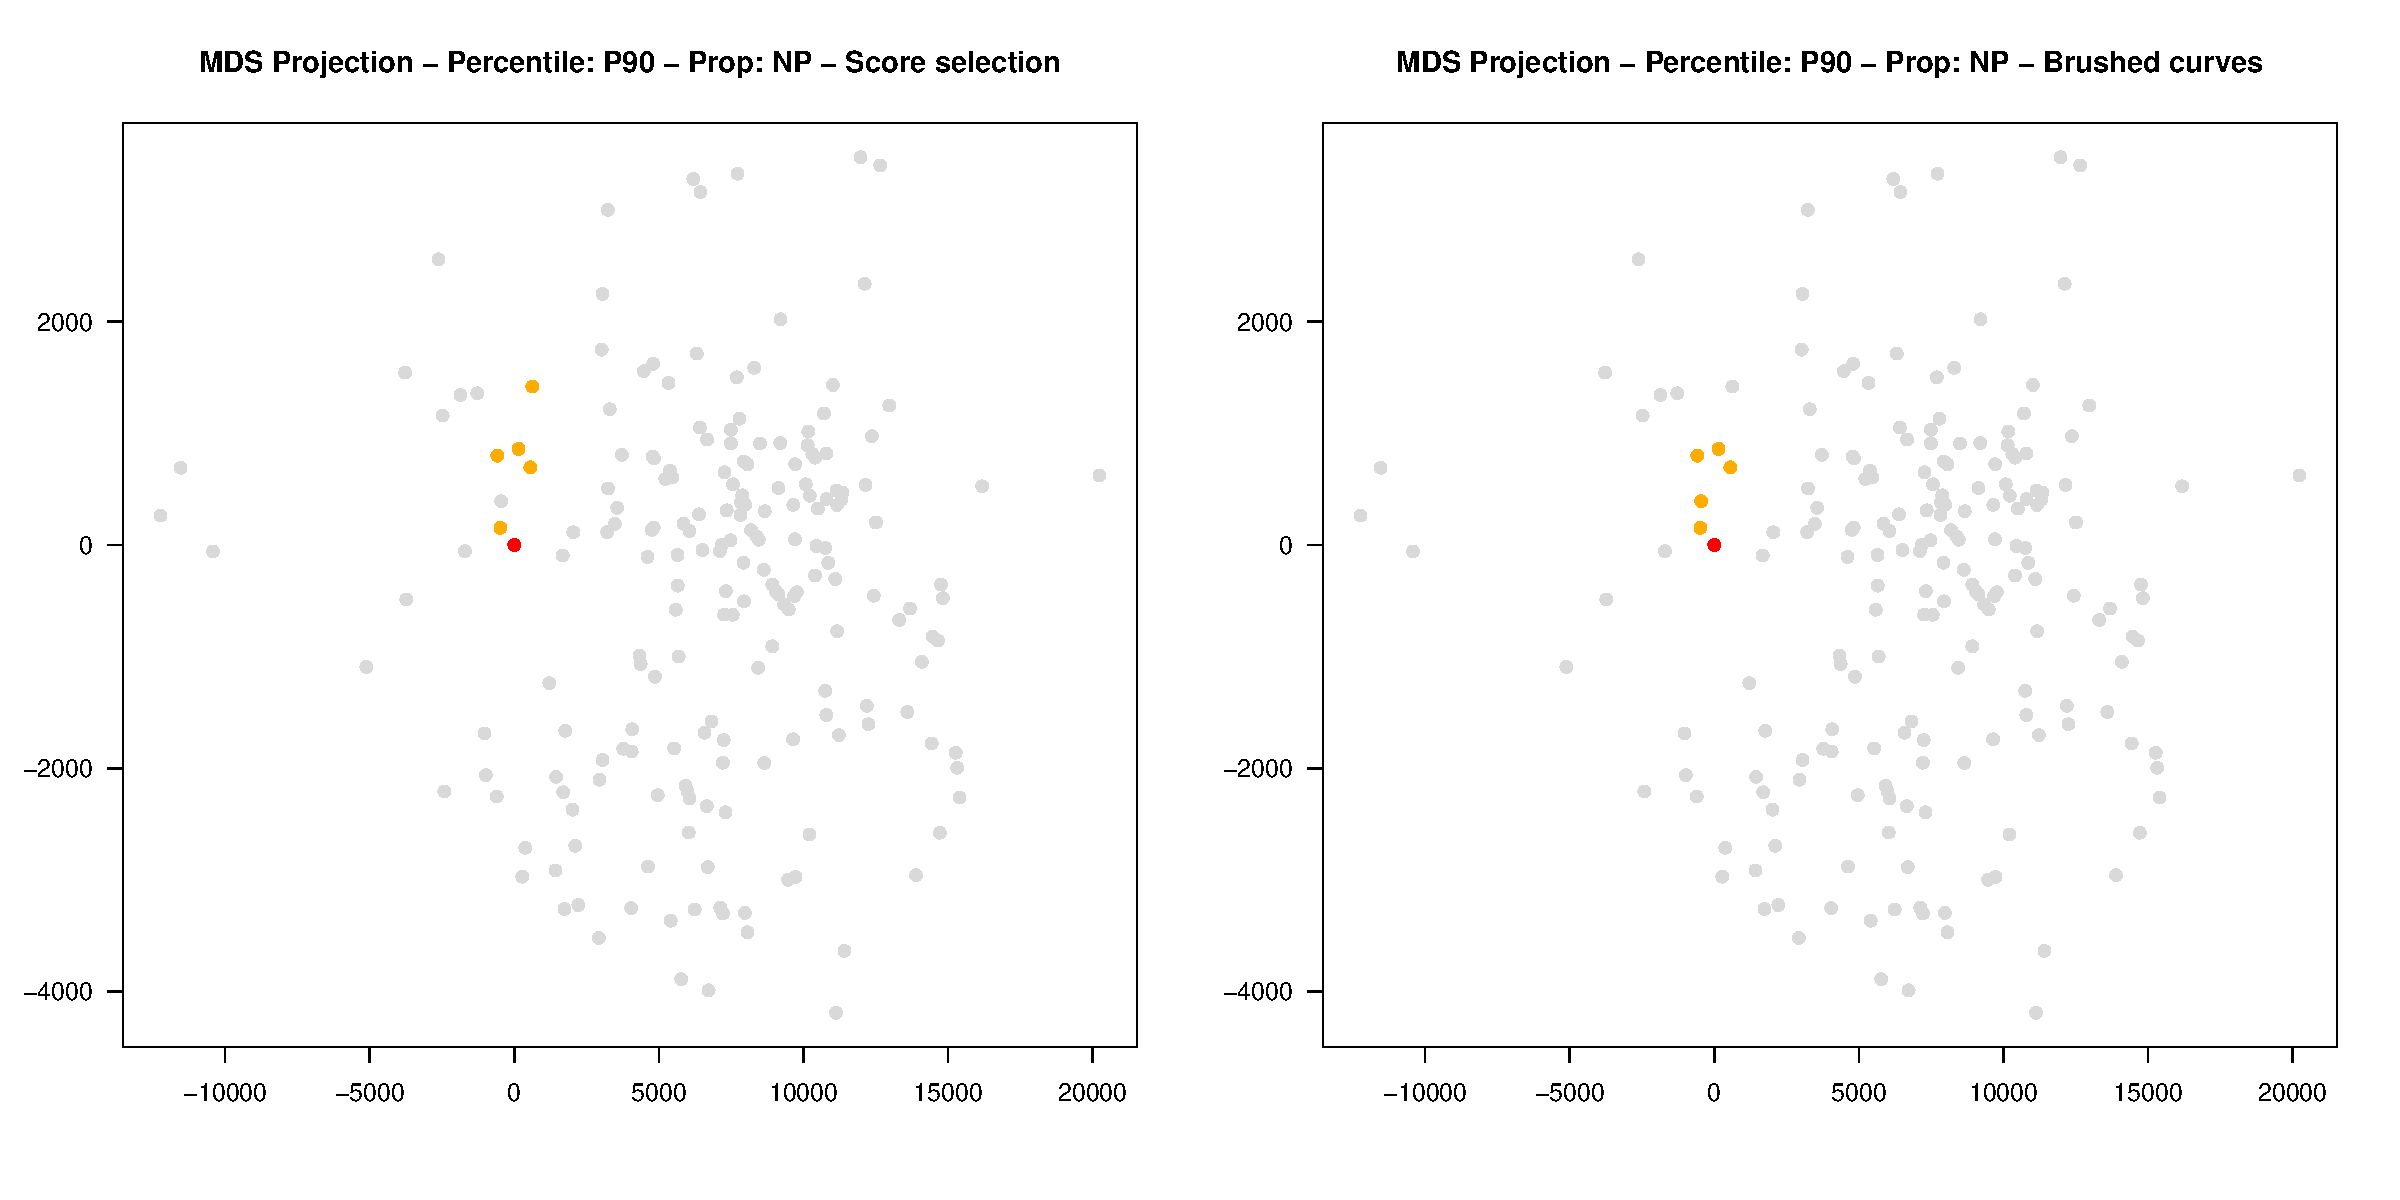
\includegraphics[width=0.88\columnwidth]{figures/mds-brush-score-p90.pdf}
  \caption{Comparative MDS projections of the sets selected by the score and manual brushing approaches.}
  \label{fig:mds-plots}
\end{figure}

As shown in Figures \ref{fig:rank-fan-brush} and \ref{fig:rank-fan-score}, the curves selected by using the brushing and linking technique similar to those selected by the score approach. For the P$_{10}$ case, the curves UNISIM\_66, UNISIM\_54, UNISIM\_156 and UNISIM\_167 were selected by both approaches; in the P$_{50}$ case, only the curve UNISIM\_45 was selected by both approaches; and for the P$_{90}$ case, the curves UNISIM\_186, UNISIM\_147, UNISIM\_58 and UNISIM\_53 were selected. These results indicate that both approaches yield good candidates. By analyzing the corresponding rank charts, both sets have very good adherence to the references, especially towards the end of the simulation, due to the weight function $w = arctan(t)$. 

When analyzing the projected locations of the curves in Figure \ref{fig:mds-plots}, both sets are located close to the reference percentiles, even though some of the projected models closest to the percentiles are consistently left out of both sets. The behavior of these models can be investigated by selecting their projections using a kNN approach on the projected models, and thus, defining a third set of candidates to be analyzed. Their comparative rank and fan charts are shown in Figure \ref{fig:rank-fan-mds}.

\begin{figure}[H]
  \centering
  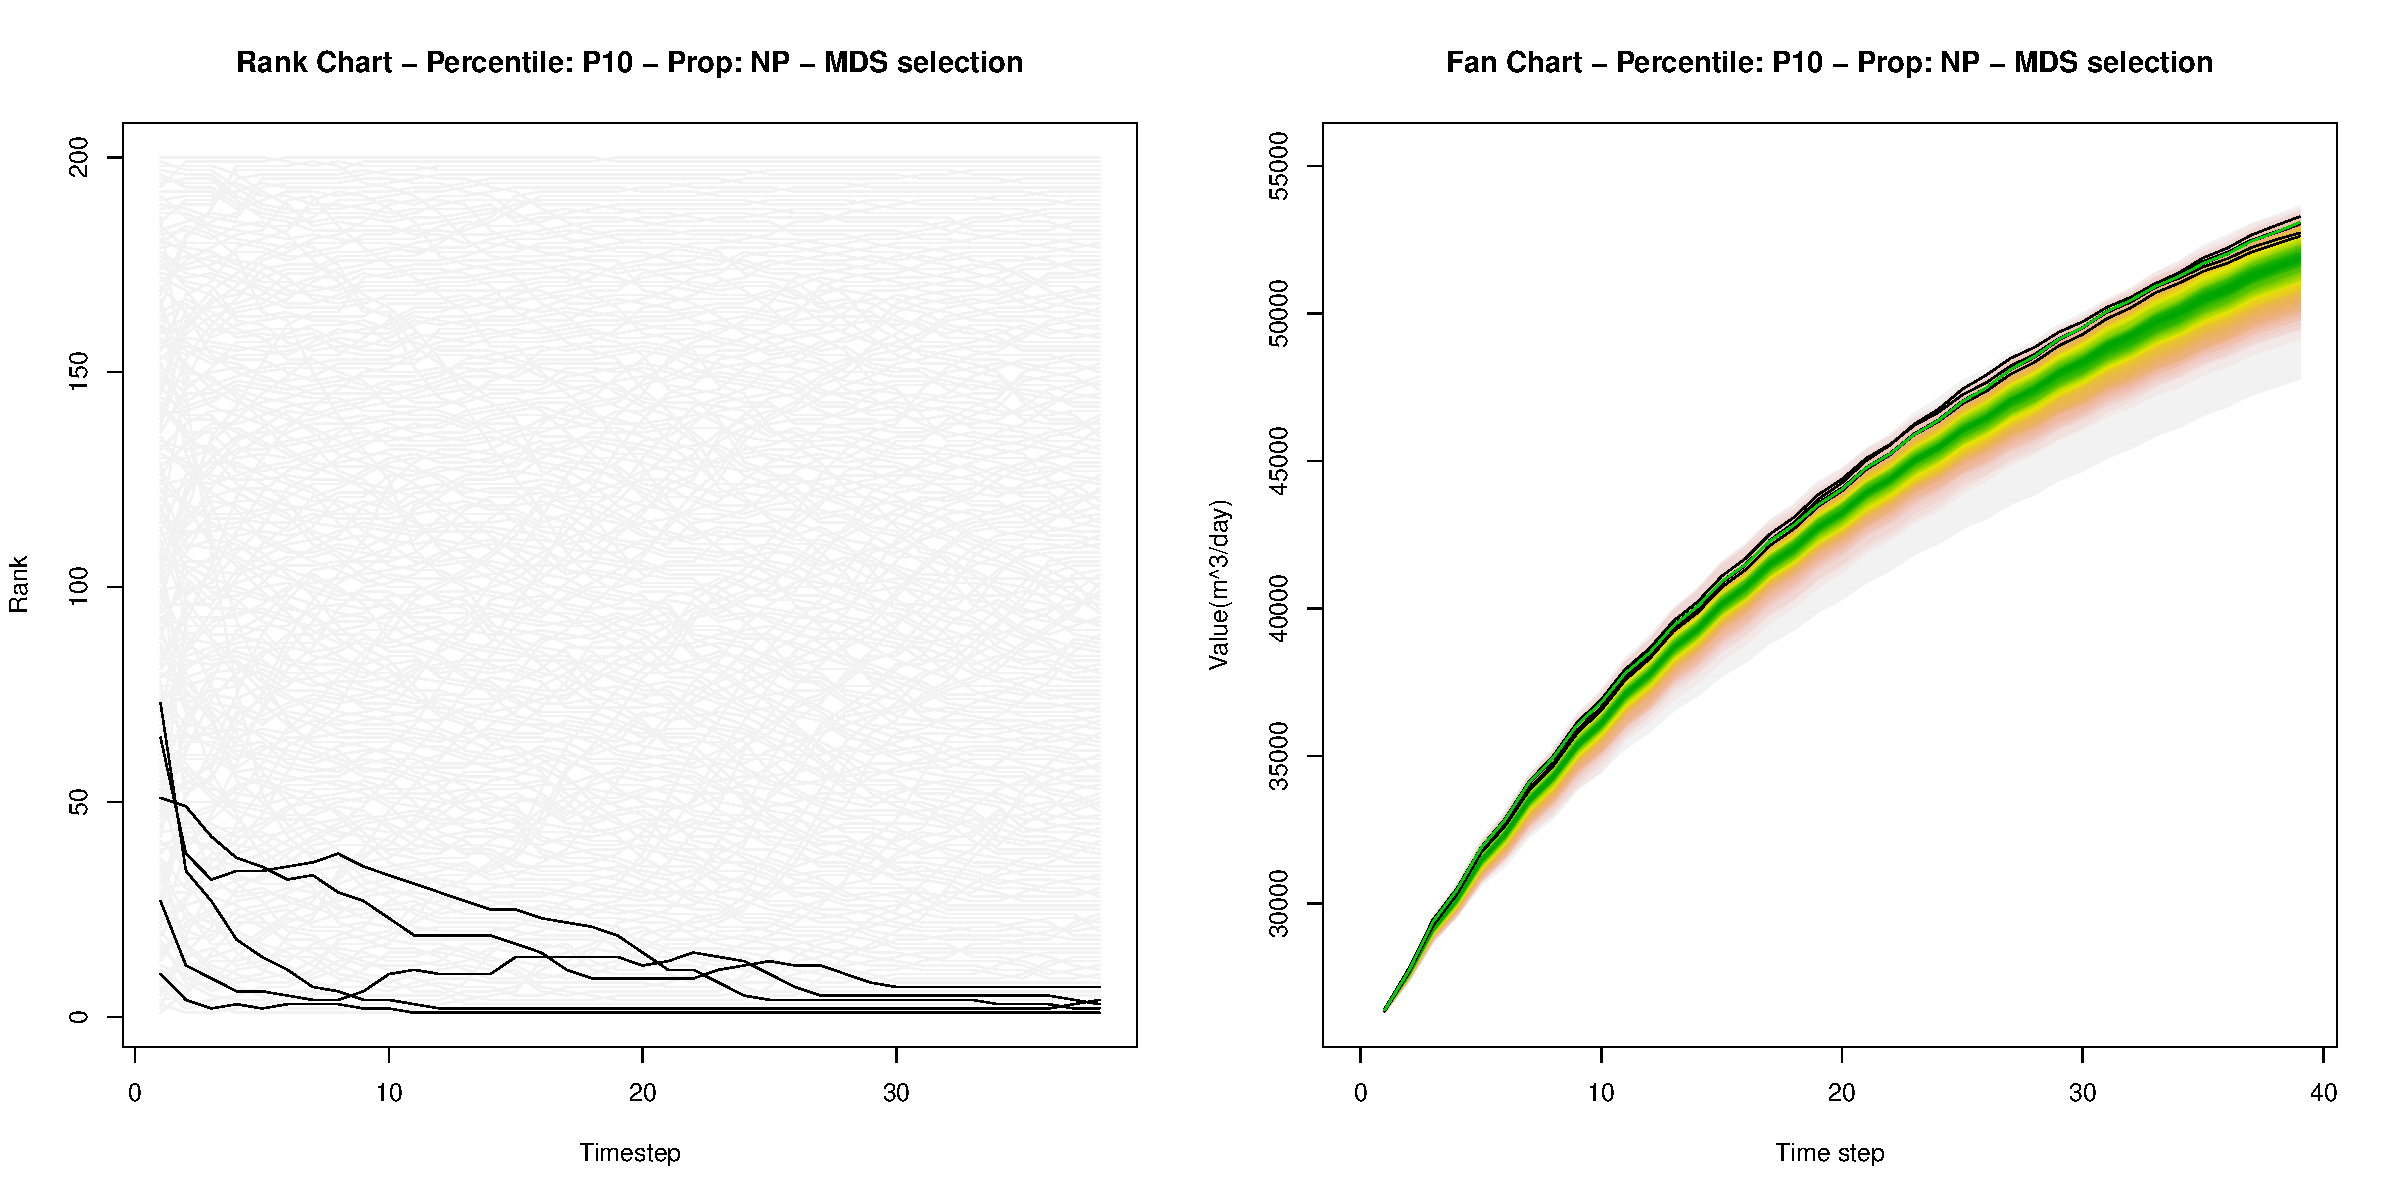
\includegraphics[width=0.8\columnwidth]{rank-fan-mds-sel-p10.pdf}
  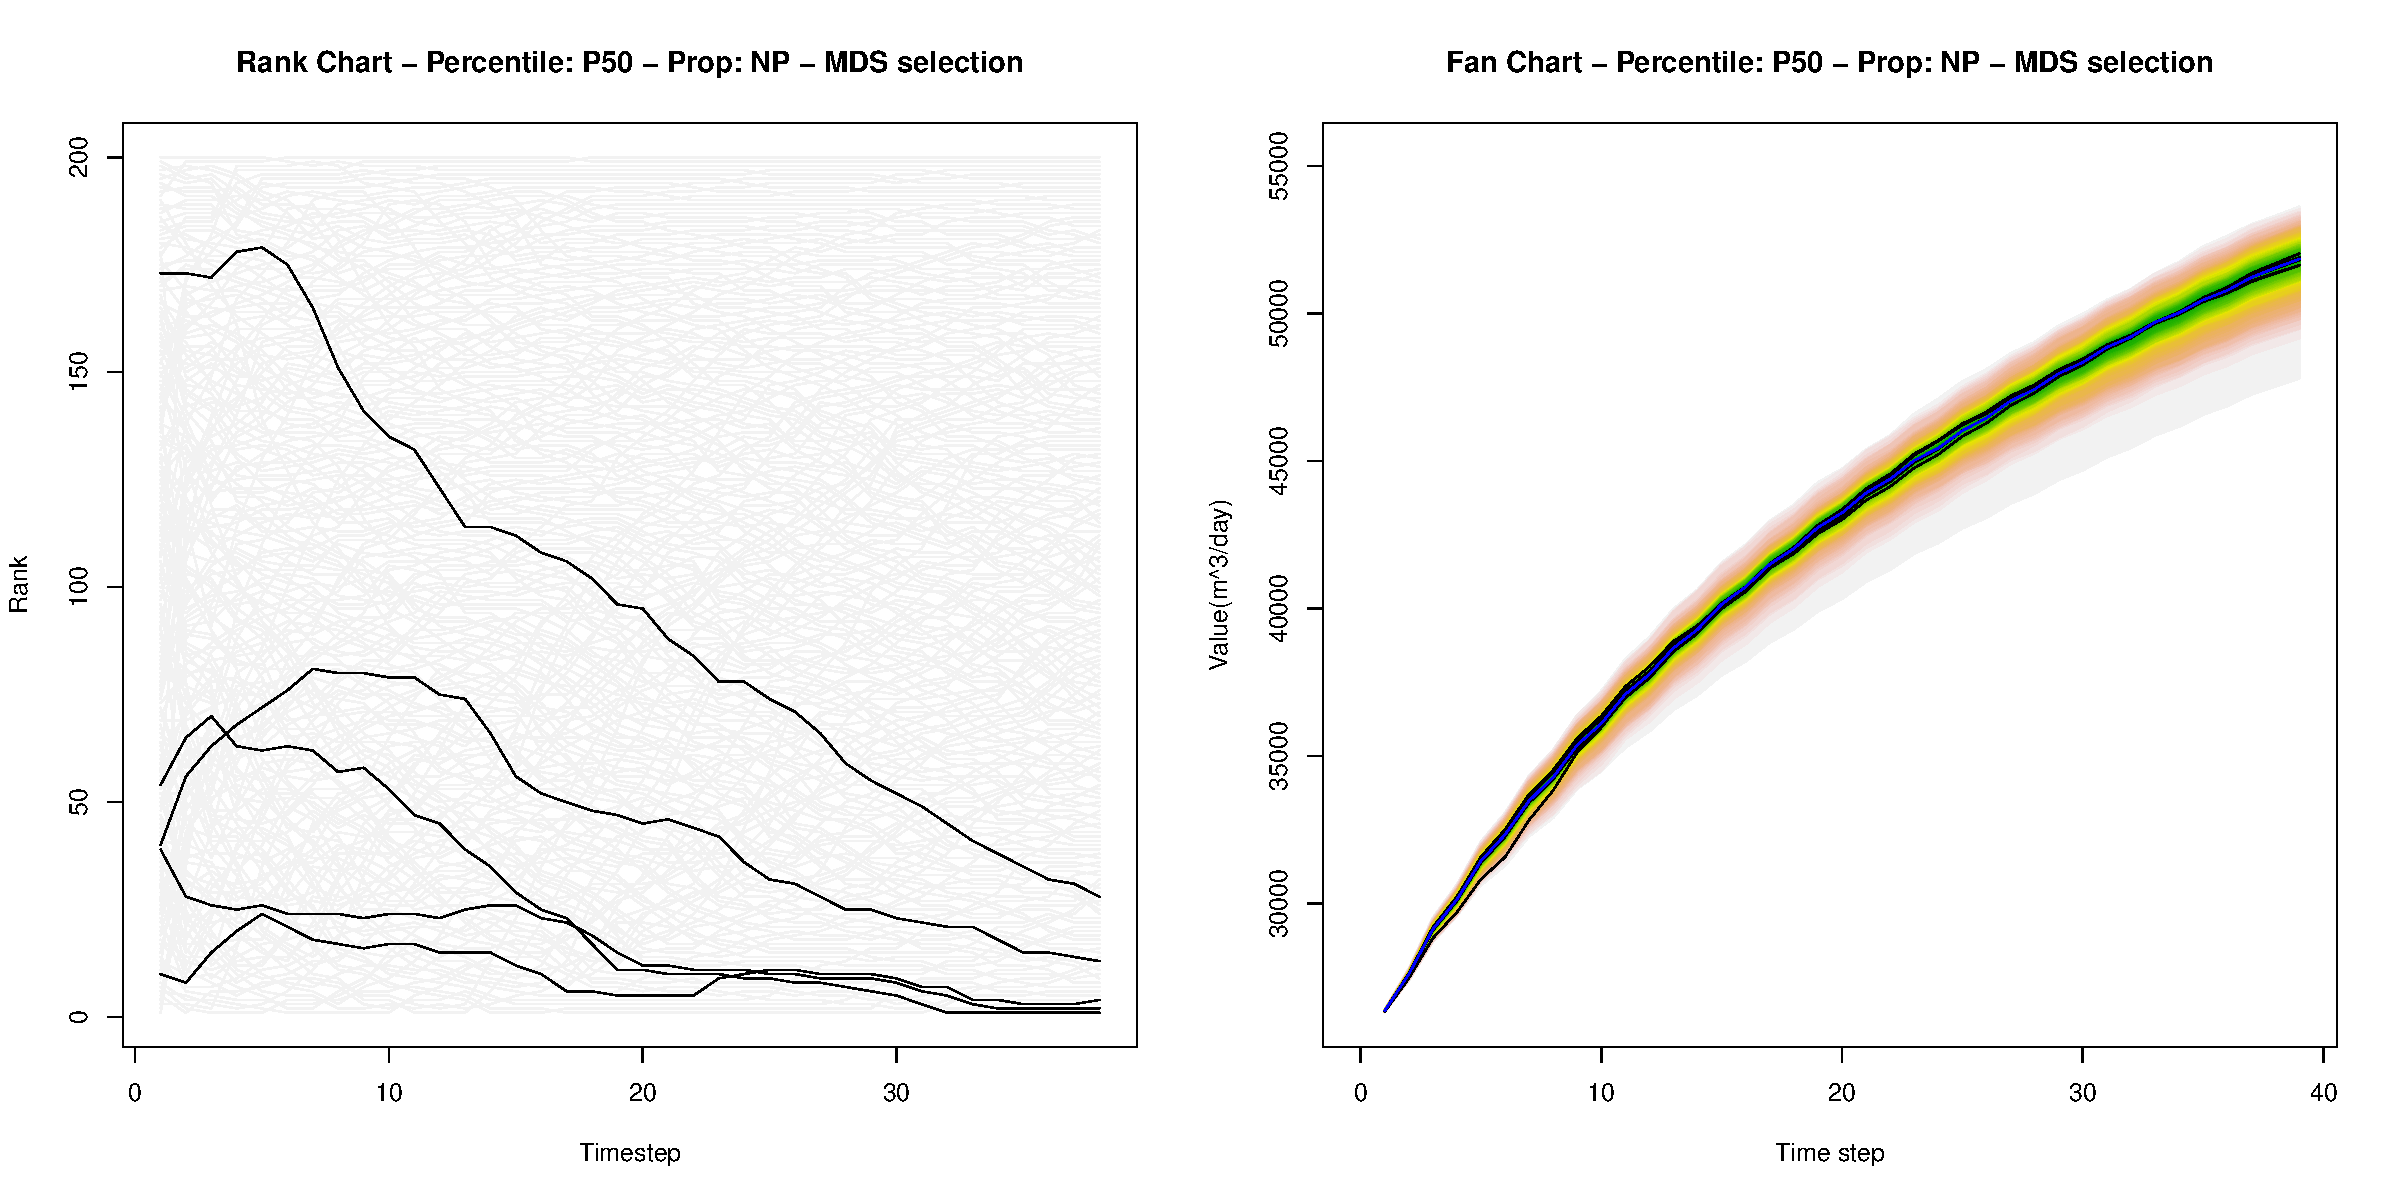
\includegraphics[width=0.8\columnwidth]{rank-fan-mds-sel-p50.pdf}
  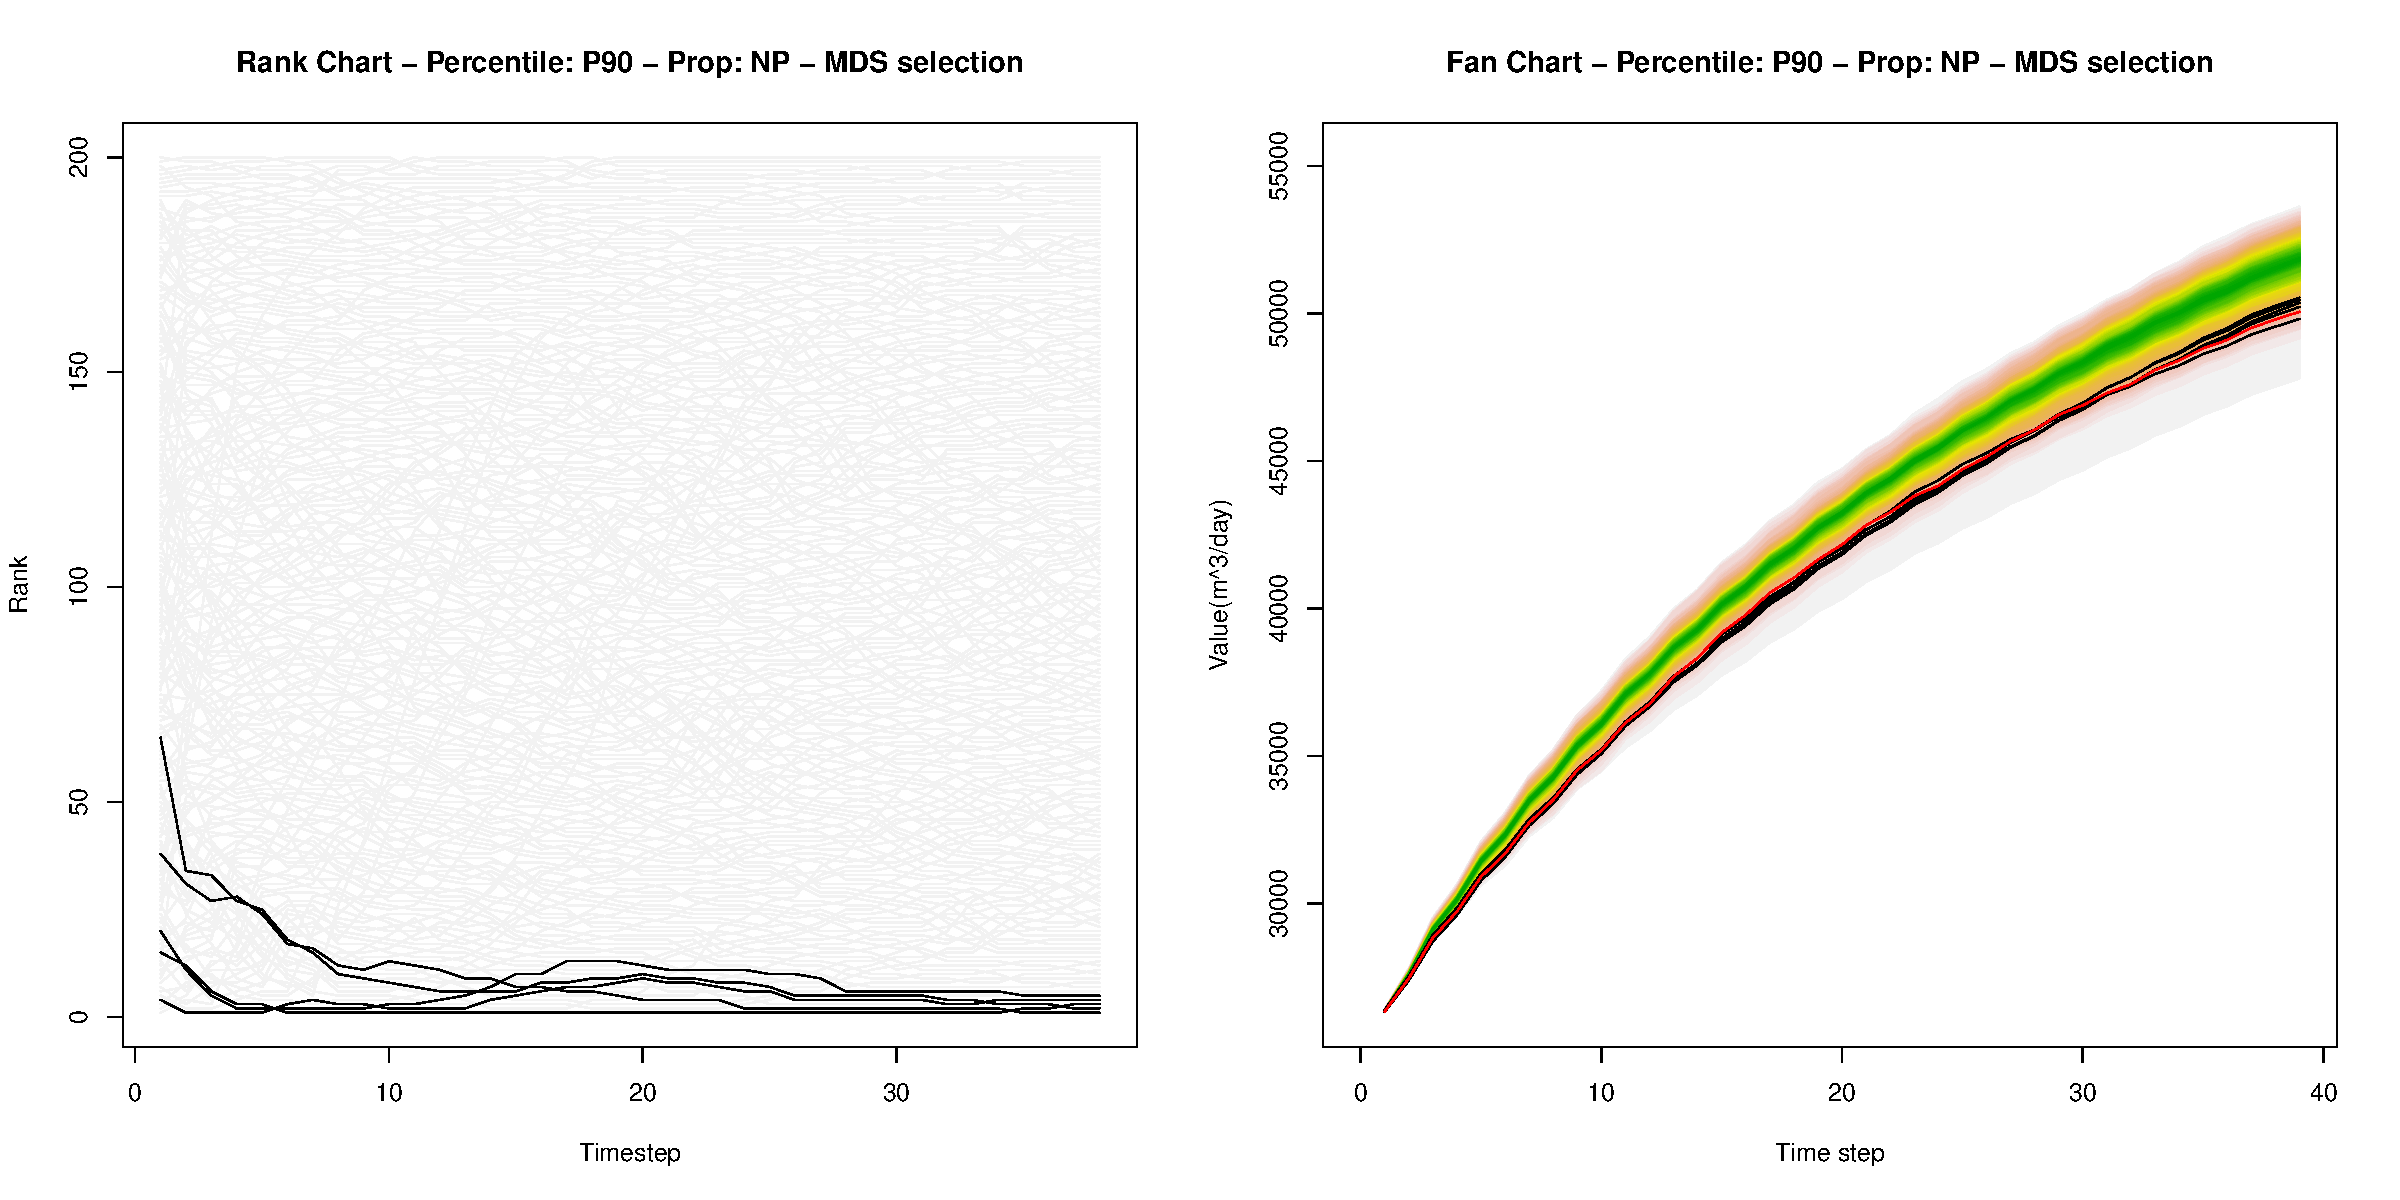
\includegraphics[width=0.8\columnwidth]{rank-fan-mds-sel-p90.pdf}
  \caption{Side-by-side rank and fan charts of the MDS projection selected curves. The selected models are UNISIM\_66, UNISIM\_159, UNISIM\_181, UNISIM\_54 and UNISIM\_156 for P$_{10}$; UNISIM\_45, UNISIM\_69, UNISIM\_194, UNISIM\_112 and UNISIM\_110 for P$_{50}$; and UNISIM\_186, UNISIM\_73, UNISIM\_58, UNISIM\_147 and UNISIM\_53 for P$_{90}$.}
  \label{fig:rank-fan-mds}
\end{figure}

The results of the MDS kNN selection shown in Figure \ref{fig:rank-fan-mds} show that the models selected by this approach are similar to the models selected by the score and brushing approaches. A notable exception is the P$_{50}$ case, where only the UNISIM\_45 model was selected on all three approaches. The models UNISIM\_194 and UNISIM\_112 were also selected both in the MDS kNN and the manual selection approaches. The models UNISIM\_69 and UNISIM\_110 selected by the MDS kNN approach have remarkably poor ranking in the beginning of the forecasted simulation time, indicating that even though the distance and ranking score are closely related, one does not necessarily imply the other. Figure \ref{fig:mds-sel} shows the MDS projection of the ensemble elements with the selected points marked. The resulting sets can be further inspected by plotting their rank charts side-by-side. Figure \ref{fig:rank-plots} shows the comparative rank charts of the sets using the reference percentiles, the corresponding fan charts are shown in Figure \ref{fig:fan-plots}.

\begin{figure}[H]
  \centering
  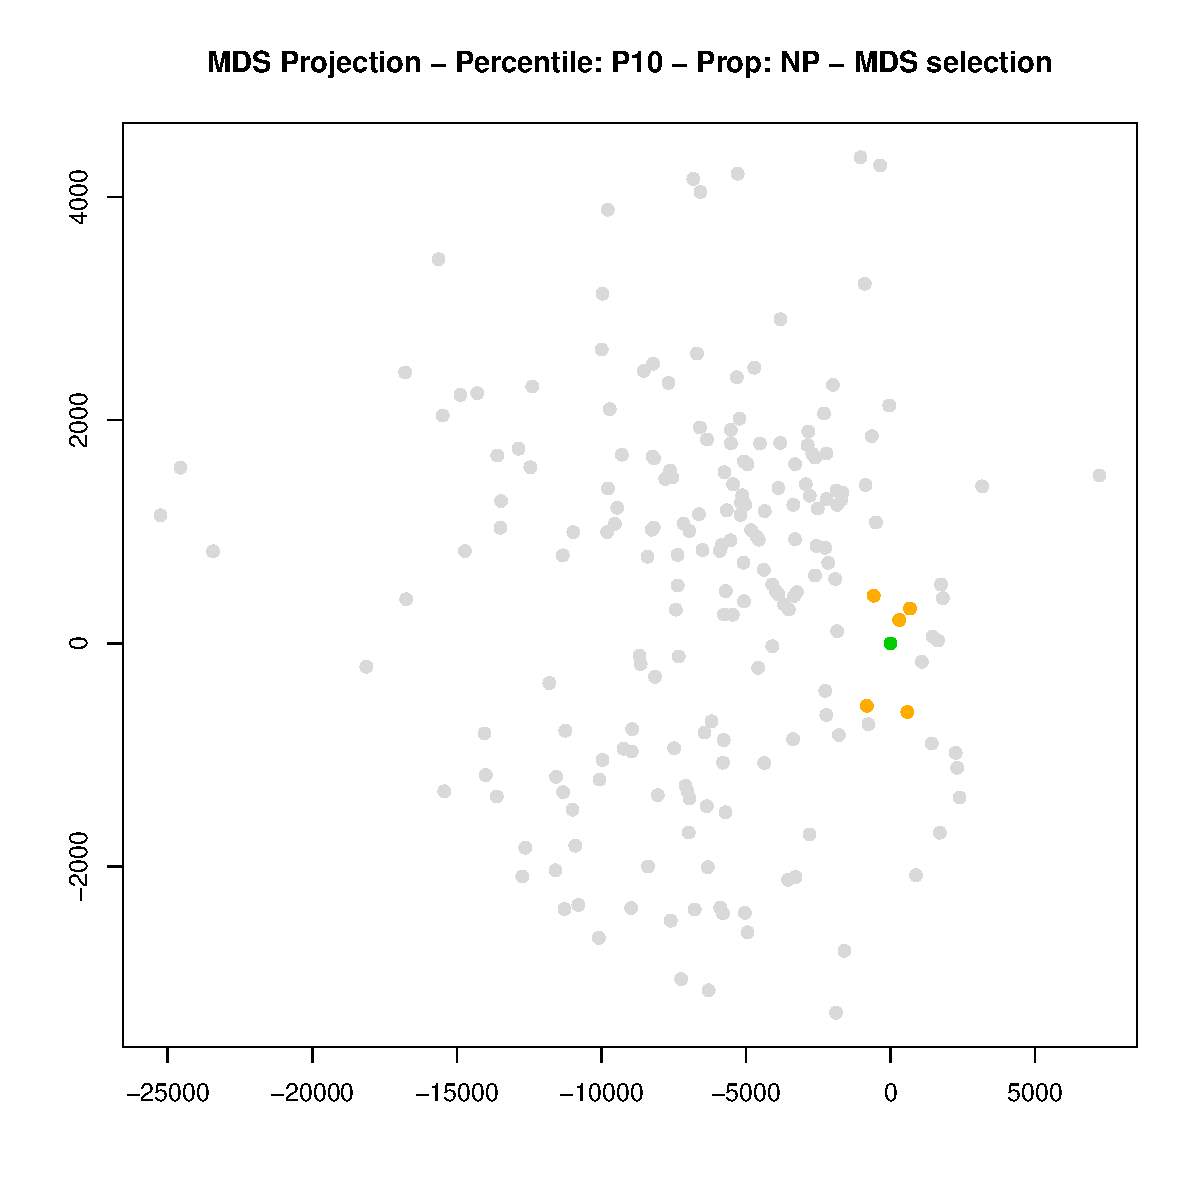
\includegraphics[height=0.49\columnwidth]{figures/mds-sel-p10.pdf}
  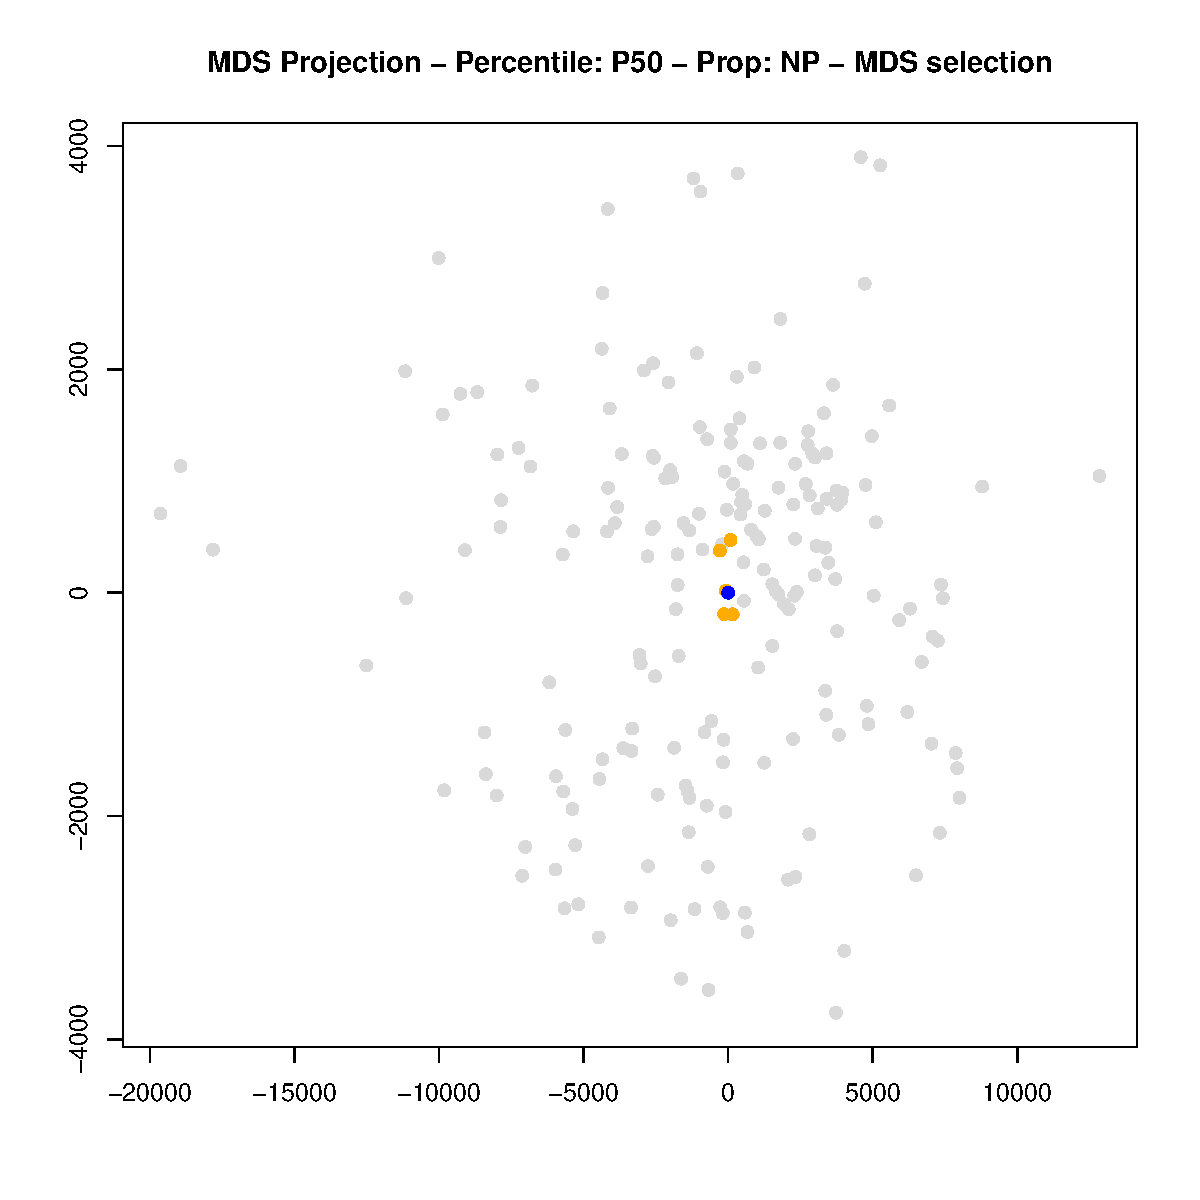
\includegraphics[height=0.49\columnwidth]{figures/mds-sel-p50.pdf}
  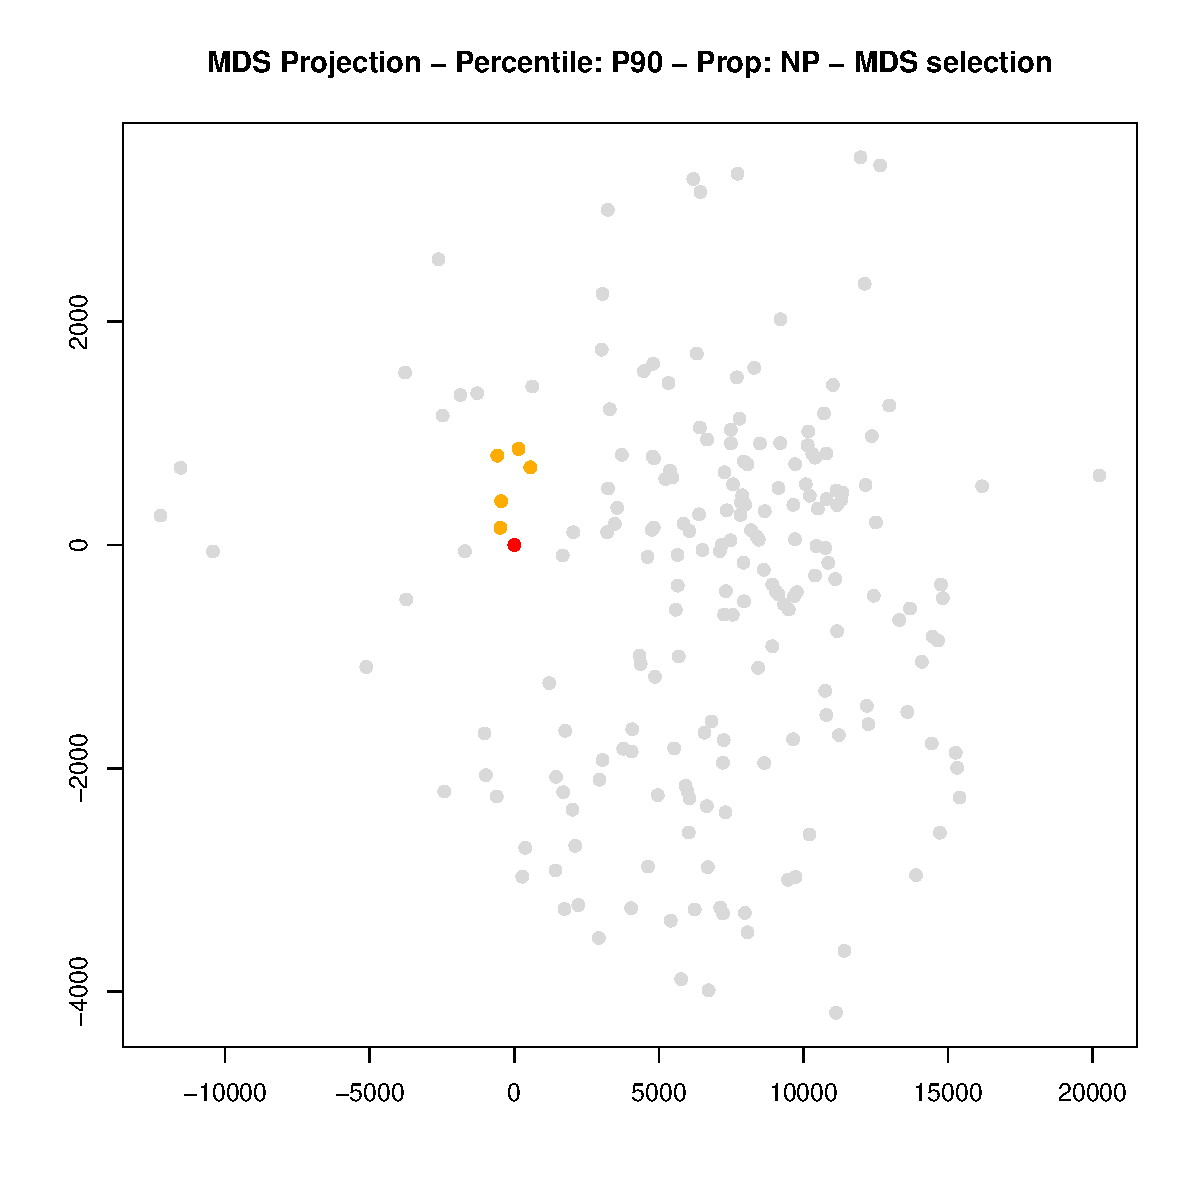
\includegraphics[height=0.49\columnwidth]{figures/mds-sel-p90.pdf}
  \caption{MDS projections of the ensemble elements with the selected entities in orange and the P$_{10}$, P$_{50}$ and P$_{90}$ models in green, blue and red respectively.}
  \label{fig:mds-sel}
\end{figure}

\begin{figure}[H]
  \centering
  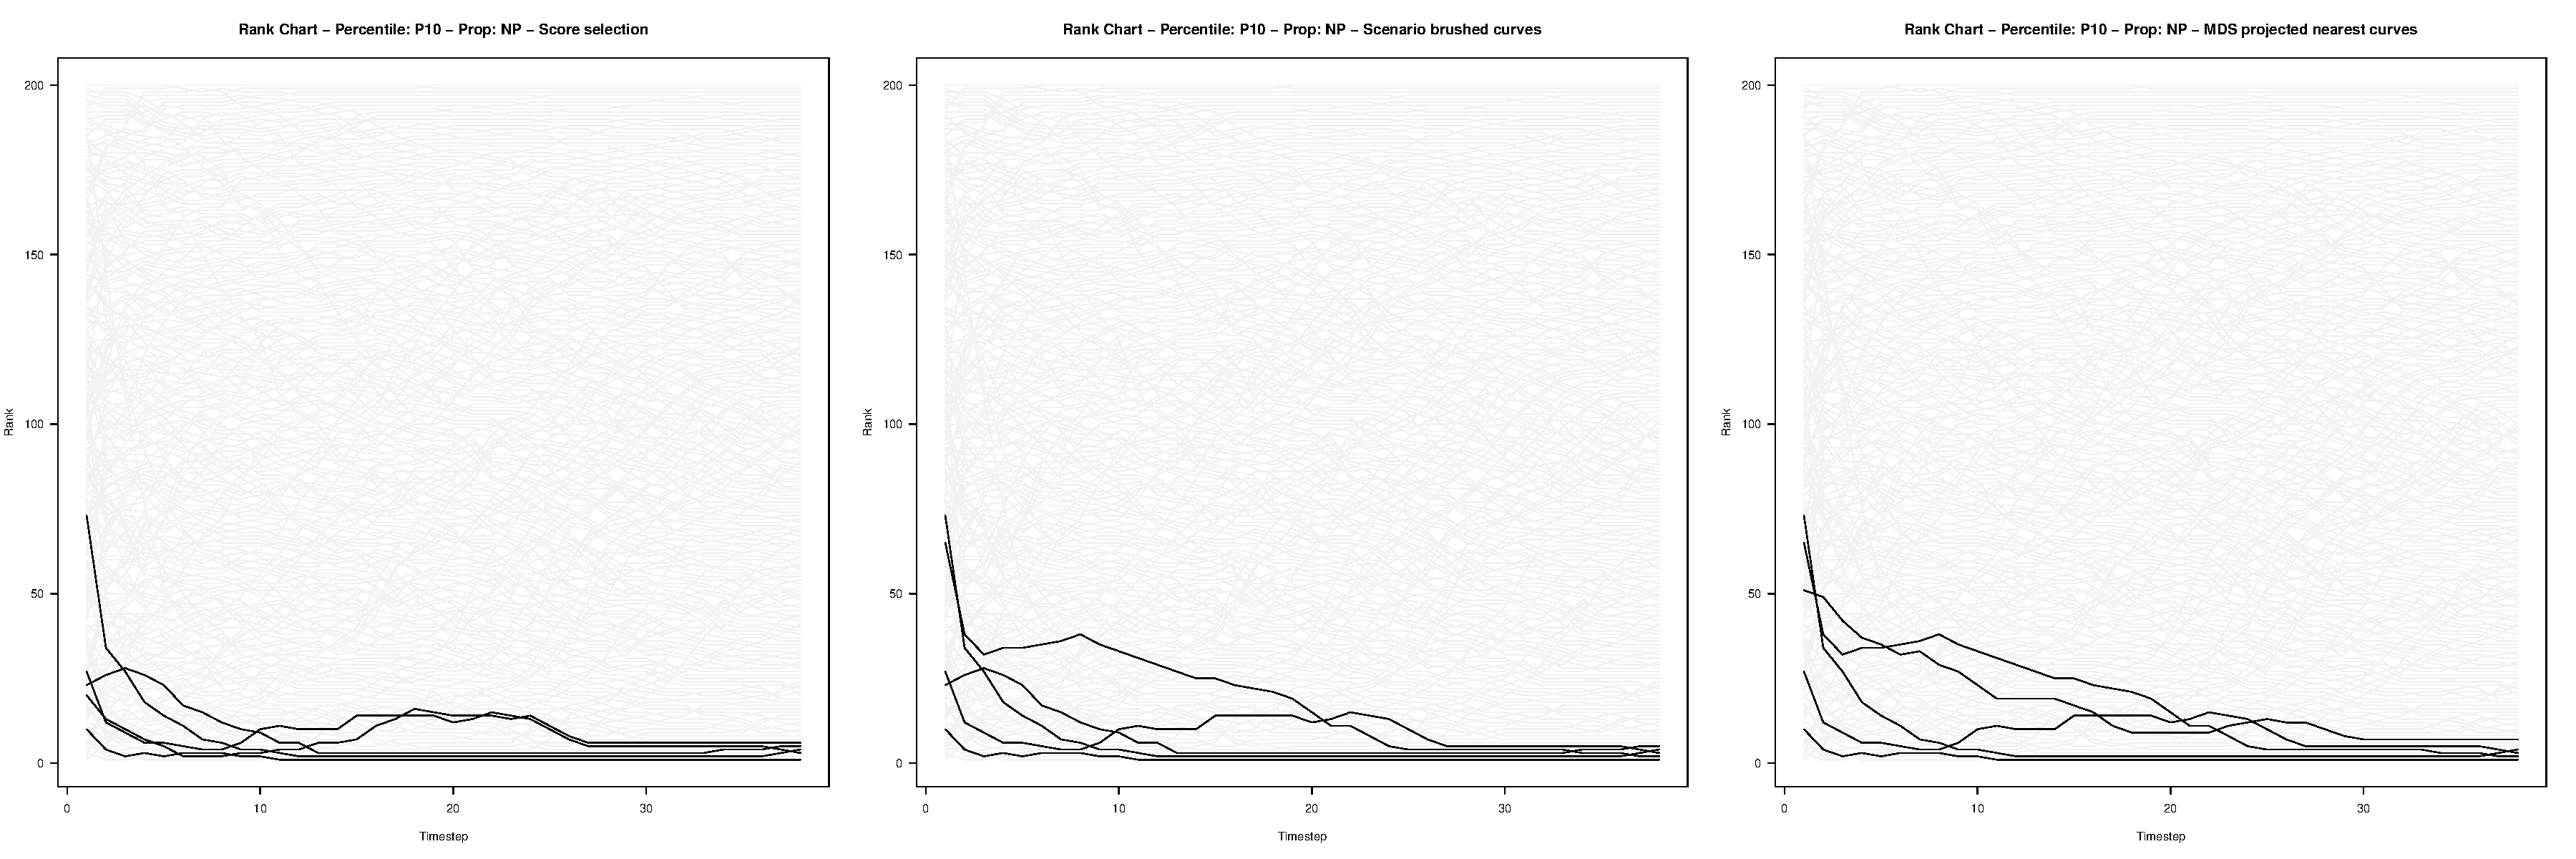
\includegraphics[width=\columnwidth]{figures/rank-score-brush-mds-p10.pdf}
  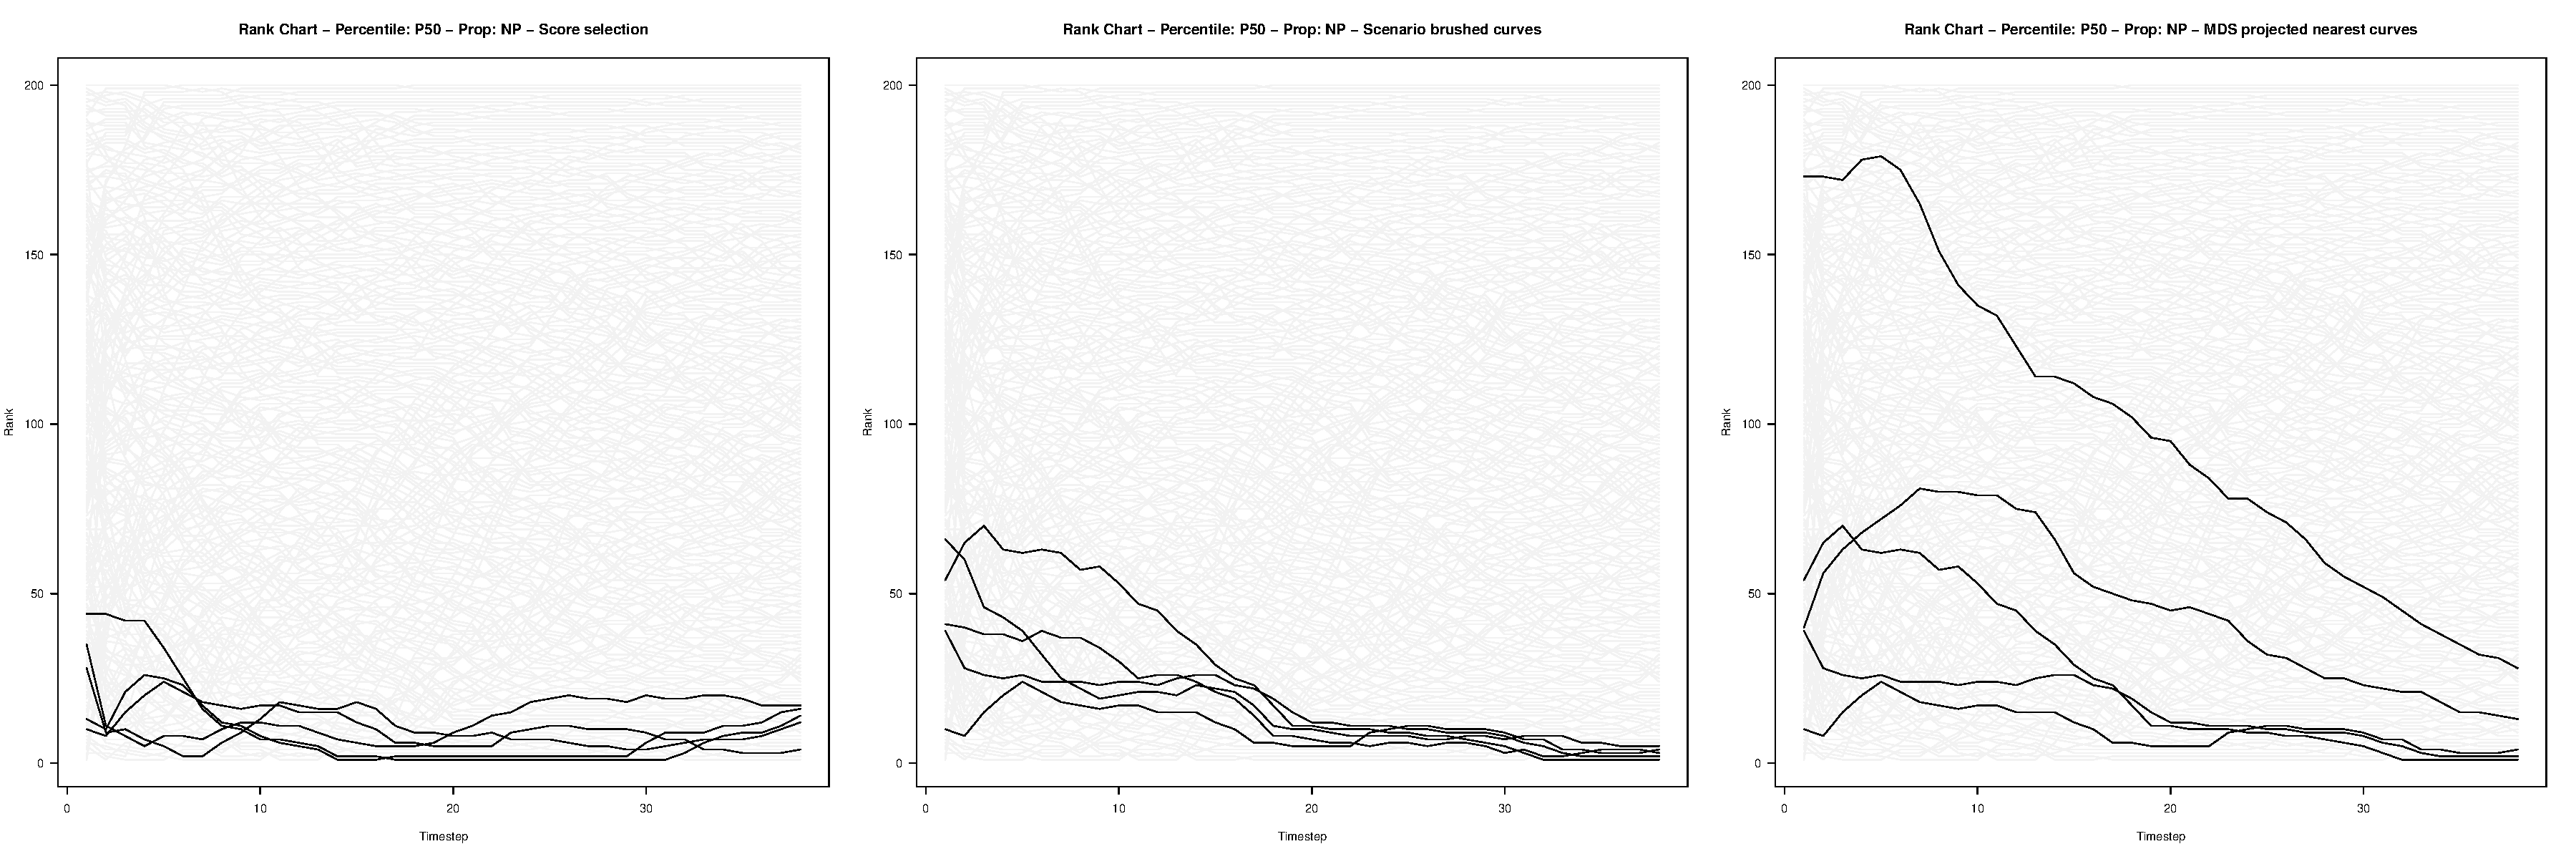
\includegraphics[width=\columnwidth]{figures/rank-score-brush-mds-p50.pdf}
  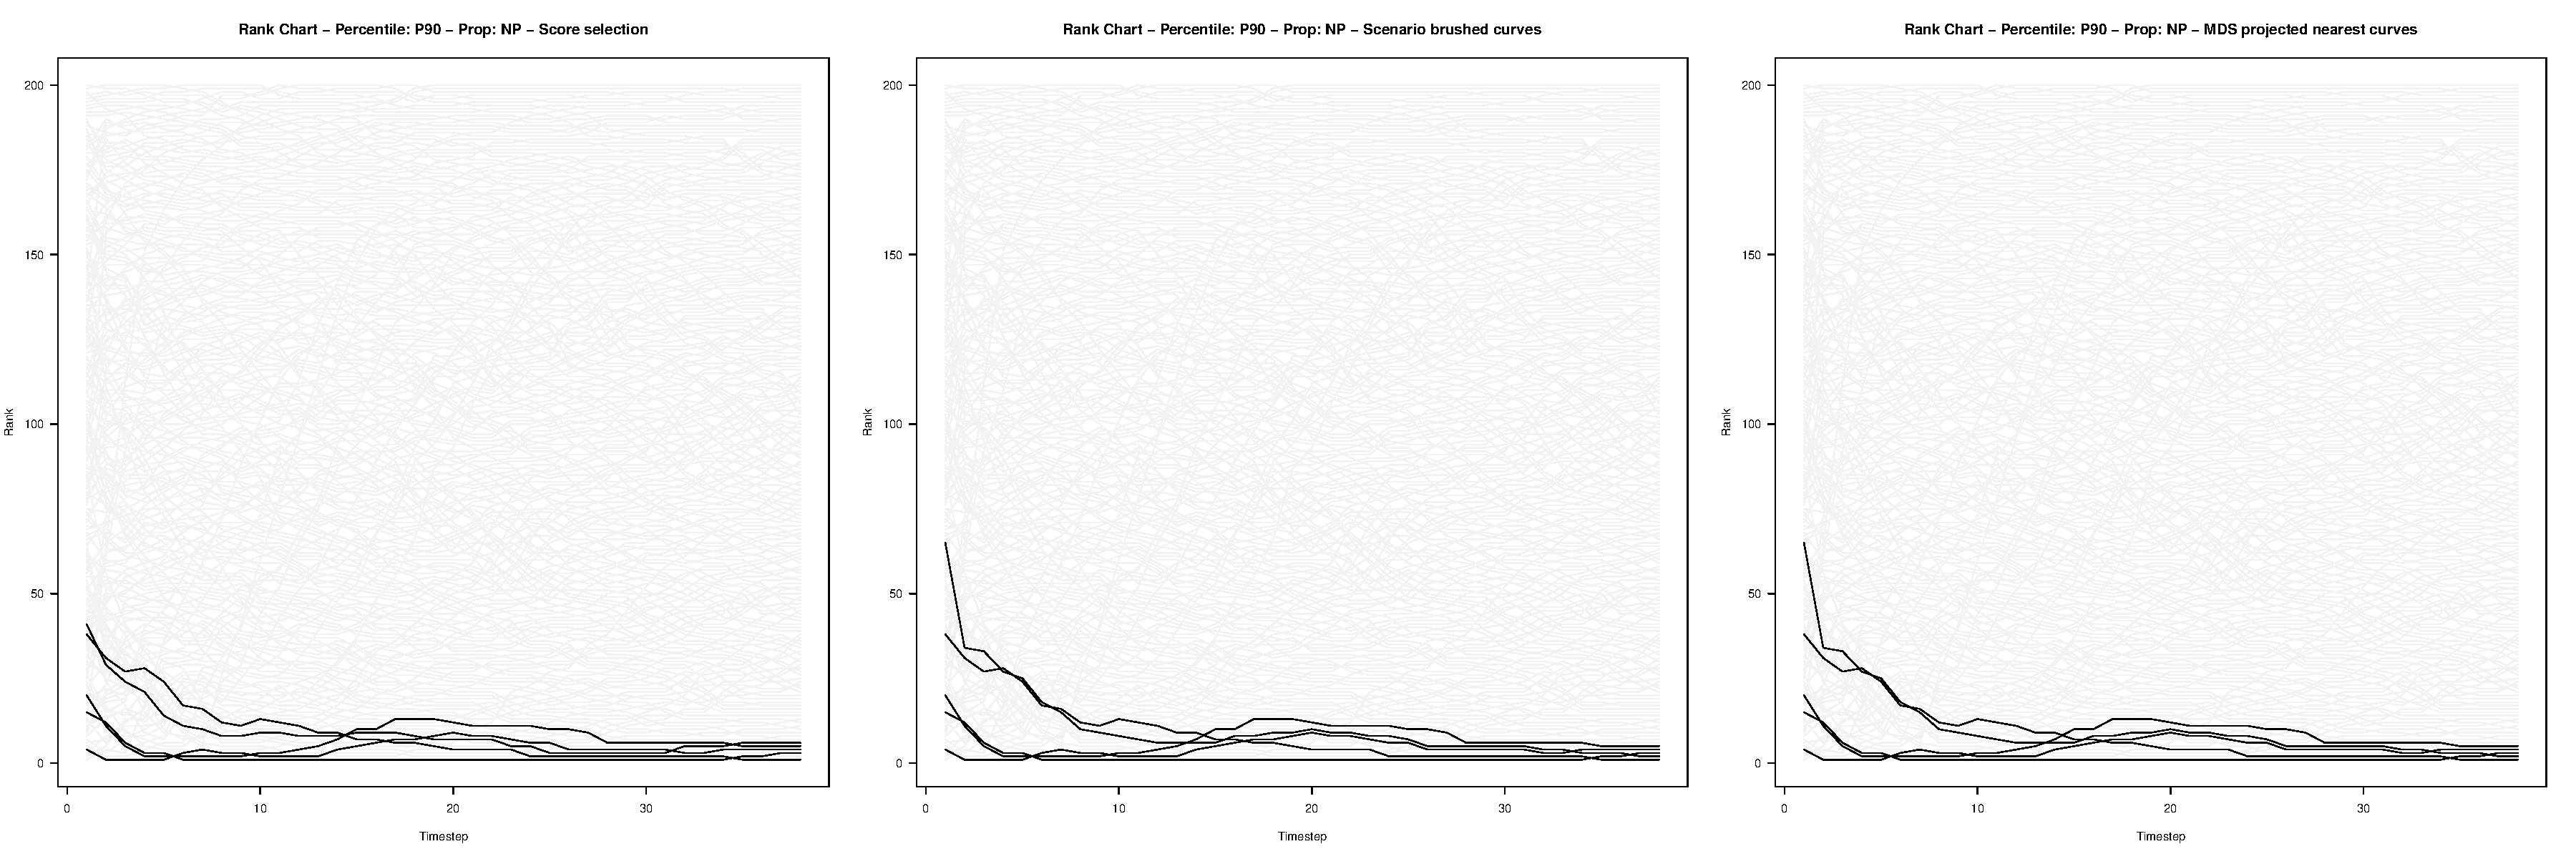
\includegraphics[width=\columnwidth]{figures/rank-score-brush-mds-p90.pdf}
  \caption{Comparative Rank Charts of the sets. The selected candidates are marked in black and the other ensemble elements are in light gray to avoid visual clutter. From top to bottom, we have the rank charts for each percentile, P$_{10}$, P$_{50}$ and P$_{90}$ respectively; and from left to right, we have the different selection methods: score-based, manual and MDS kNN.}
  \label{fig:rank-plots}
\end{figure}

\begin{figure}[H]
  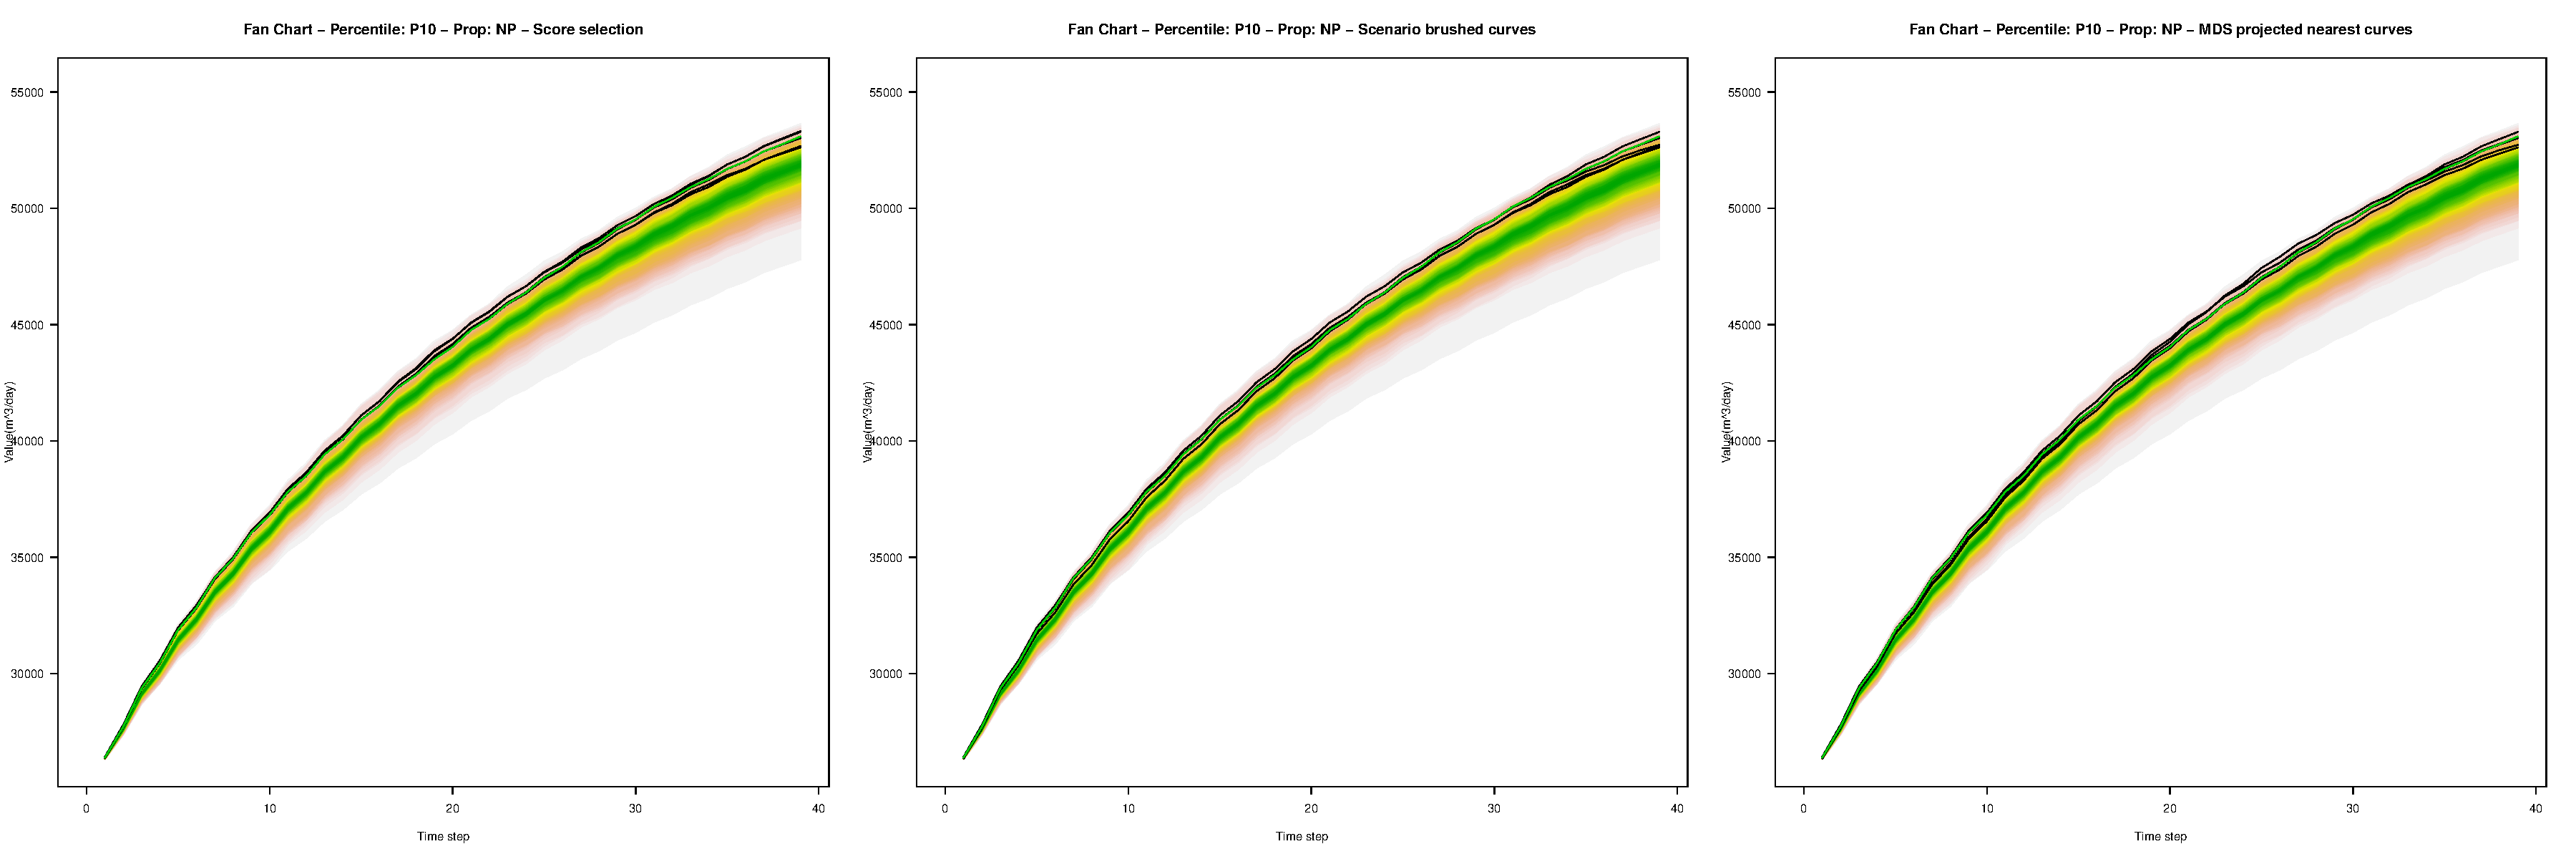
\includegraphics[width=\columnwidth]{figures/fanchart-score-brush-mds-p10.pdf}
  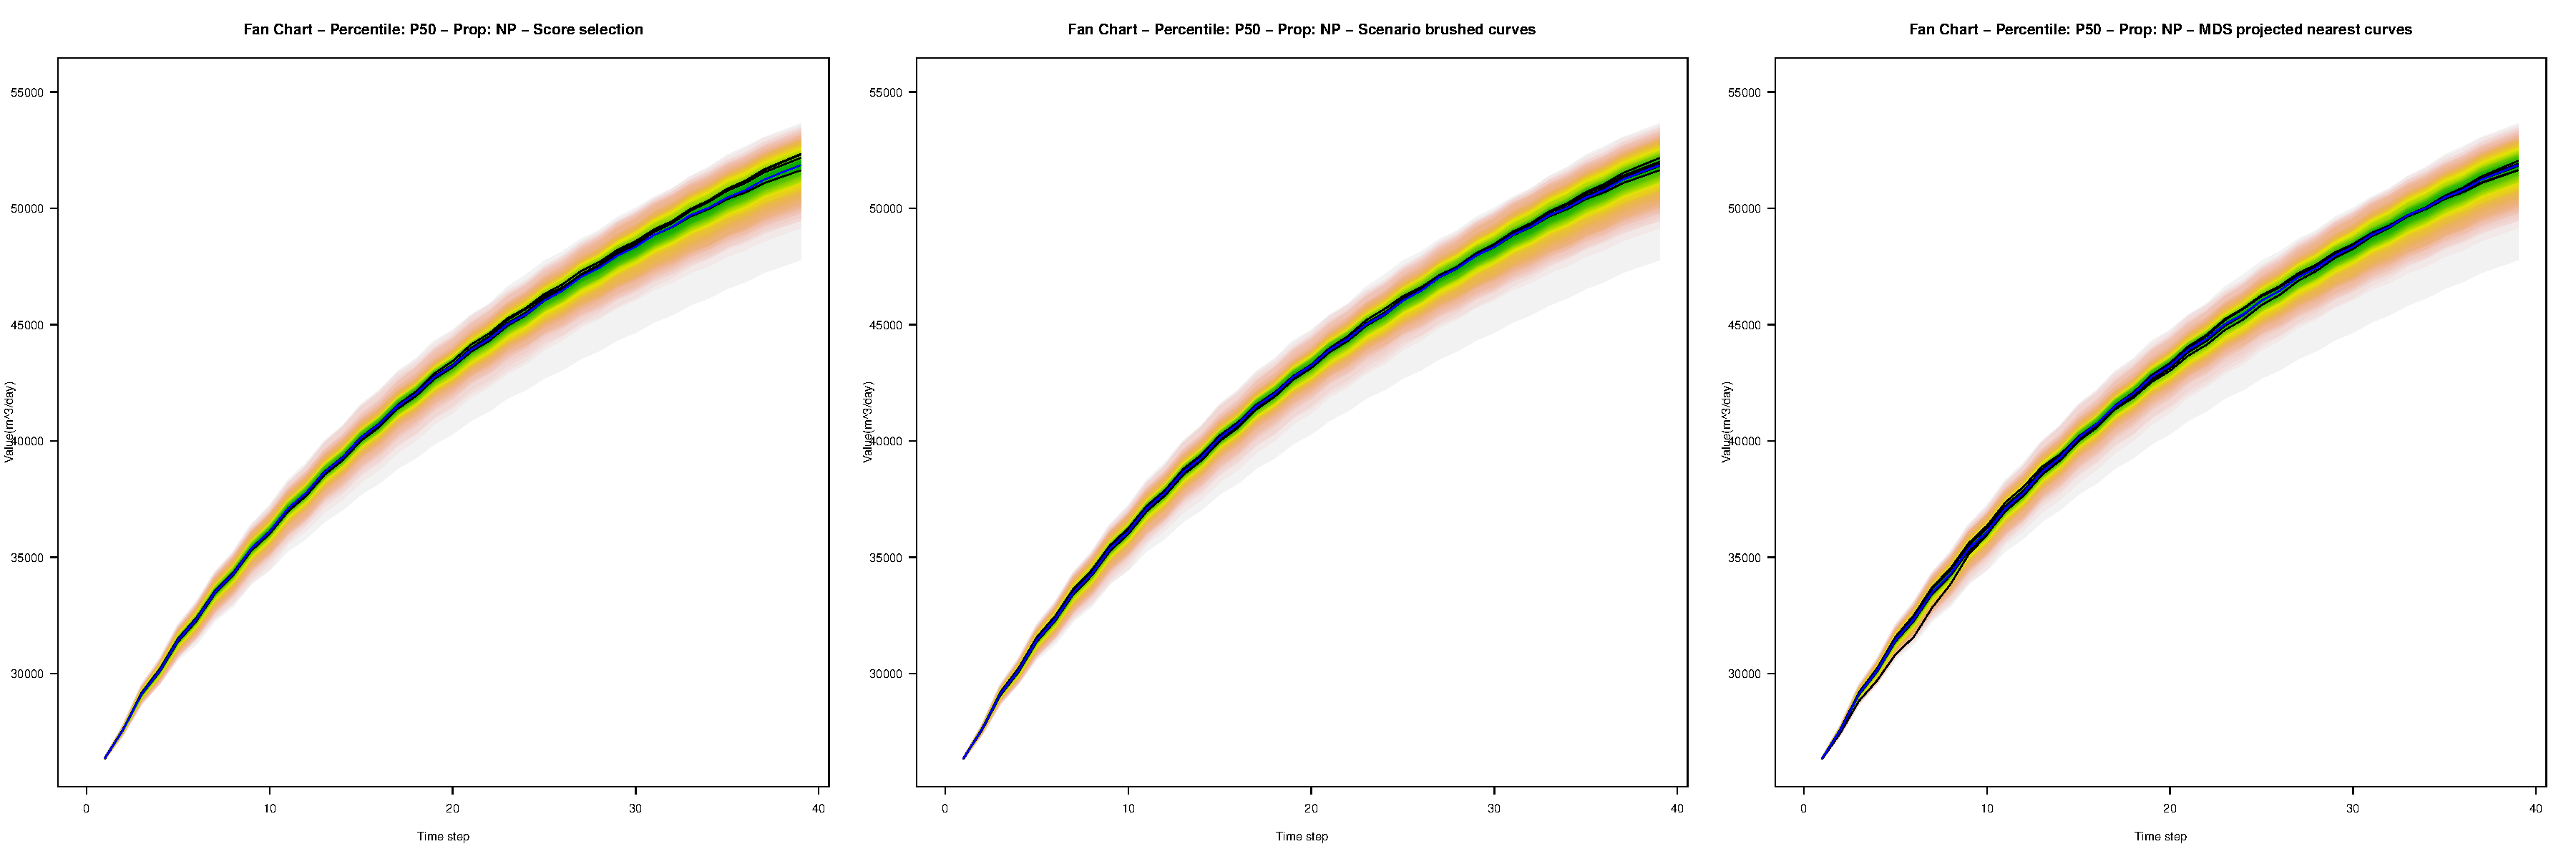
\includegraphics[width=\columnwidth]{figures/fanchart-score-brush-mds-p50.pdf}
  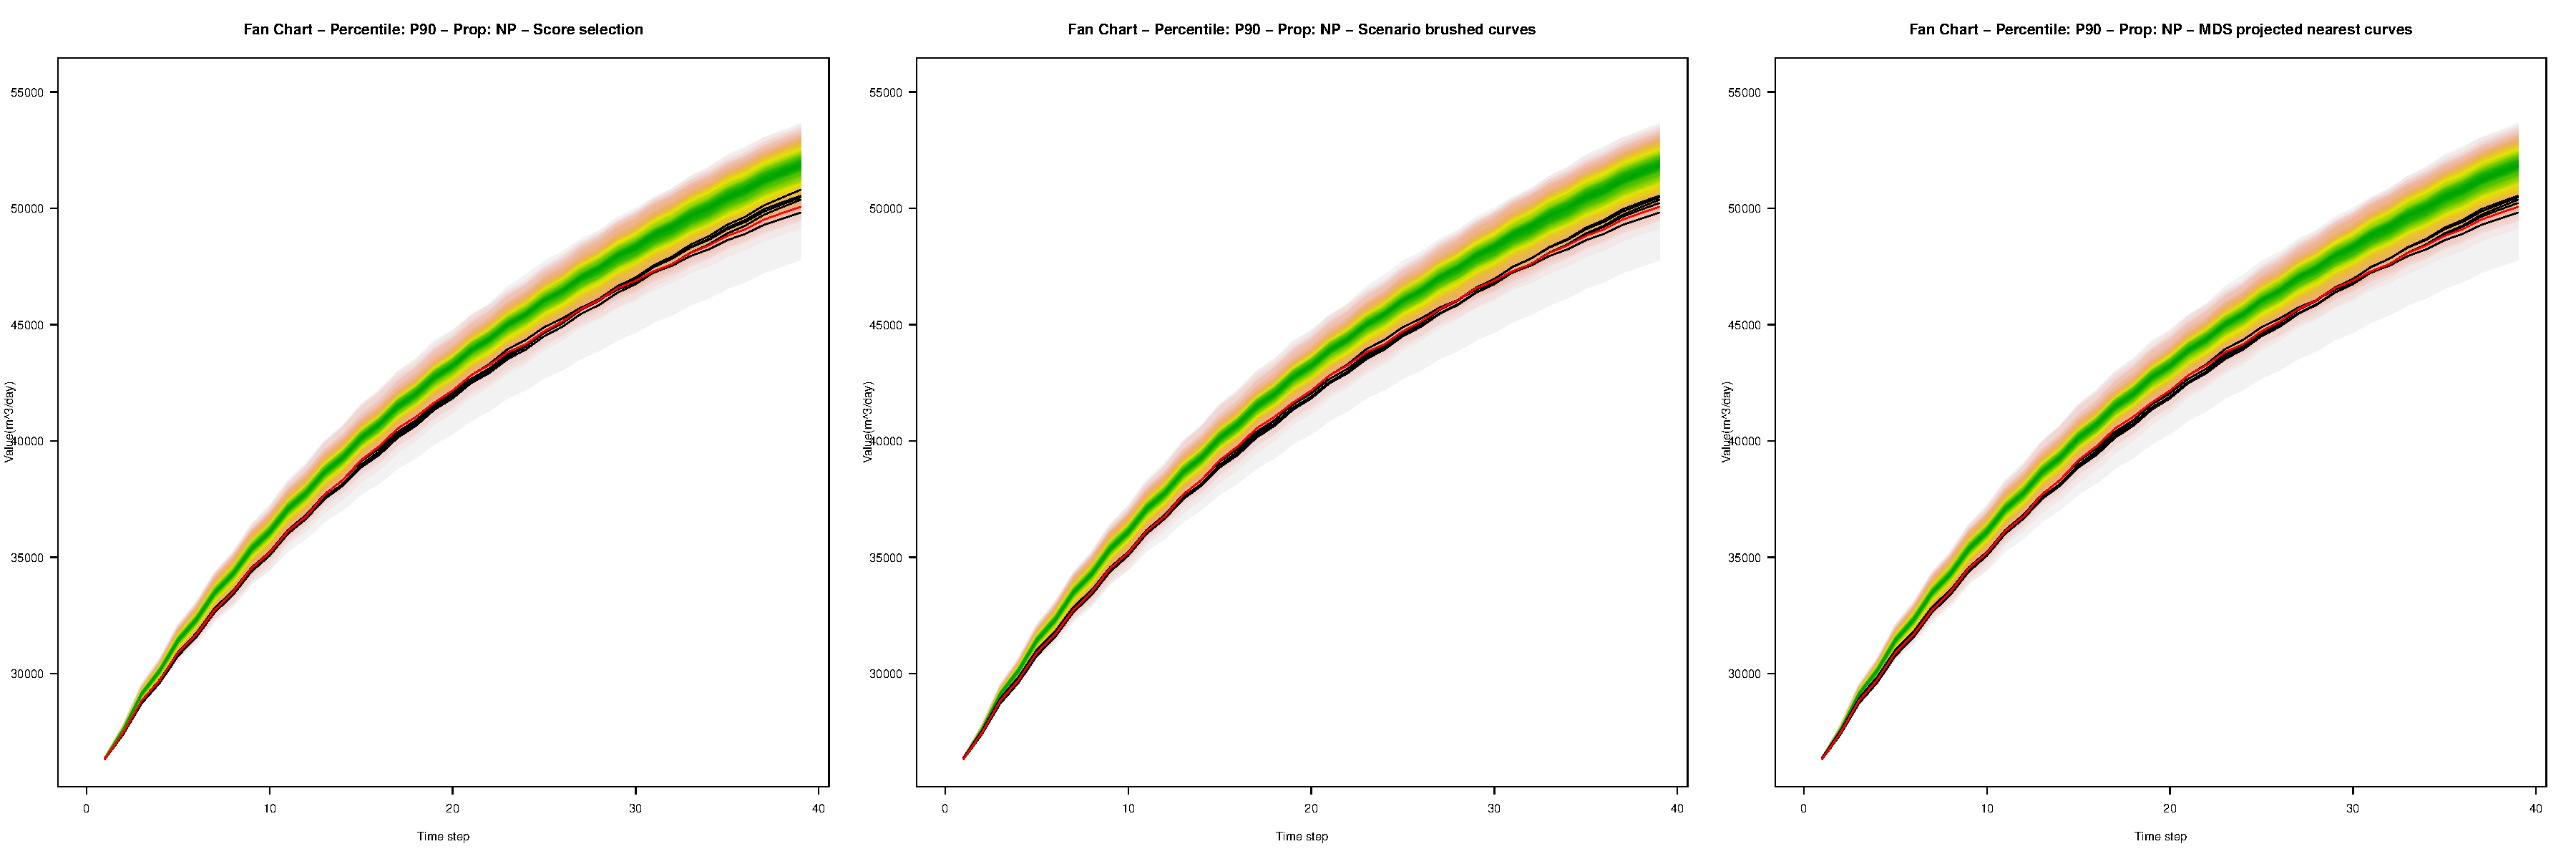
\includegraphics[width=\columnwidth]{figures/fanchart-score-brush-mds-p90.pdf}
  \caption{Comparative Fan Charts of the sets selected by each approach. From top to bottom, we have the fan charts for each percentile, P$_{10}$, P$_{50}$ and P$_{90}$ respectively; and from left to right, we have the different selection methods: score-based, manual and MDS kNN.}
  \label{fig:fan-plots}
\end{figure}

%[FIXME]
%As shown in Figure \ref{fig:fan-plots}, the curves from set 2 are closer to their reference percentiles marked in blue when compared to the curves from set 1. This result is remarkably evident when comparing the P$_{50}$ charts, where the first set's spread is considerably higher than that of the second set, especially towards the end of the forecast. This effect is also indicated by the corresponding rank charts in Figure \ref{fig:rank-plots}.


%%%%%%%%%%%%%%%%%%%%%%%%%%%%%%%%%%%%%%%%%%%%%%%%%%%%%%%%%%%%%%%%%%%%%%%%%%%%%%

\section{Discussion}
\label{sec:discussion}

%TODO: Fazer uma análise numérica das distâncias das curvas selecionadas automaticamente e manualmente.
%TODO: Fazer um tabela listando os modelos selecionados pelo brushing e pela função de score? Incluir as distâncias das curvas de referência?
%TODO: Fazer uma comparação qualitativa com os trabalhos anteriores.

The main motivation for our work is the fact that the selection approaches found in the literature do not handle time series data at all. In the case of the MinMax approach \cite{selection-sarma:2013} or Meira et al.'s \cite{meira:2016}, their approaches handle only the latest production value from each reservoir model. We hyphotesized that the evolution of a system must be taken into consideration when selecting the representative models, and a failure to take this into account may lead to a poorer selection. Consider the models shown in Figure \ref{fig:ecdf-NP}; these models were selected by calculating the P$_{10}$, P$_{50}$ and P$_{90}$ of NP using the data described in Section \ref{sec:experiments}. The models with values closest to the percentiles were selected as representative models, their rank and fan charts are shown in Figure \ref{fig:rank-fan-ecdf}. The MDS projection of the selected models is shown in Figure \ref{fig:mds-ecdf}. The three selected models are close to the percentiles only on the last simulation time step, they have an overall poor ranking throughout the simulation and are distant from the percentiles, as shown in the MDS projections in Figure \ref{fig:mds-ecdf}. Therefore, using only a single value for the selection process may yield models that fit only that value, but have an overall poor adherence to the calculated percentiles.

\begin{figure}[H]
  \centering
  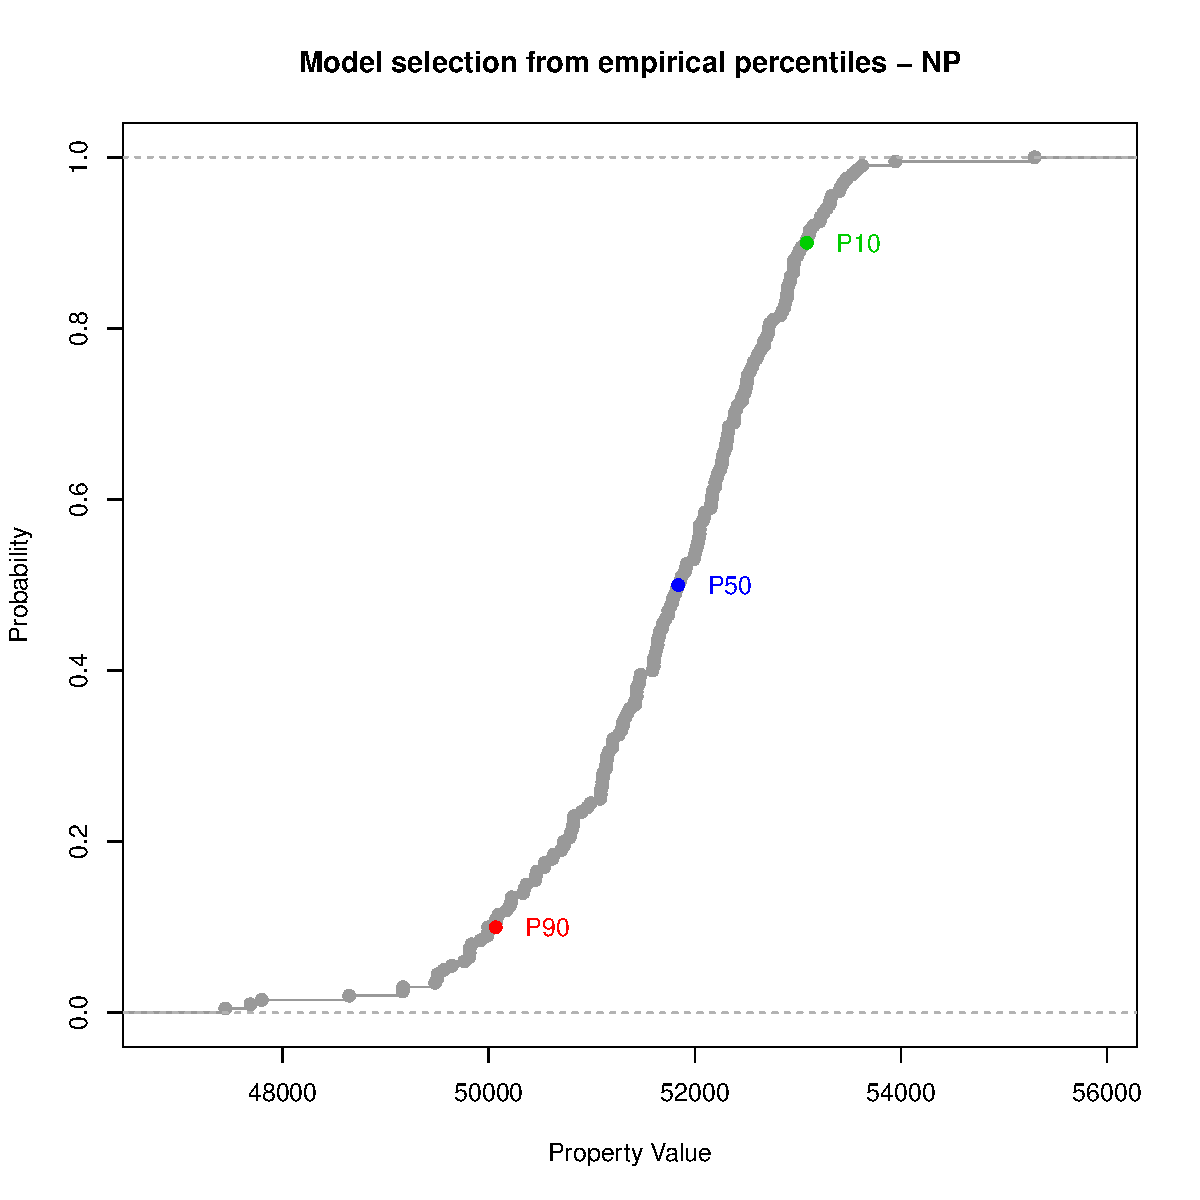
\includegraphics[width=\columnwidth]{ecdf-NP.pdf}
  \caption{Empirical cumulative probability distribution of the latest production values of the cumulative oil production of UNISIM-I-H. The P$_{10}$, P$_{50}$ and P$_{90}$ models are marked in green, blue and red and correspond to the models UNISIM\_96, UNISIM\_4 and UNISIM\_172 respectively.}
  \label{fig:ecdf-NP}
\end{figure}

\begin{figure}[H]
  \centering
  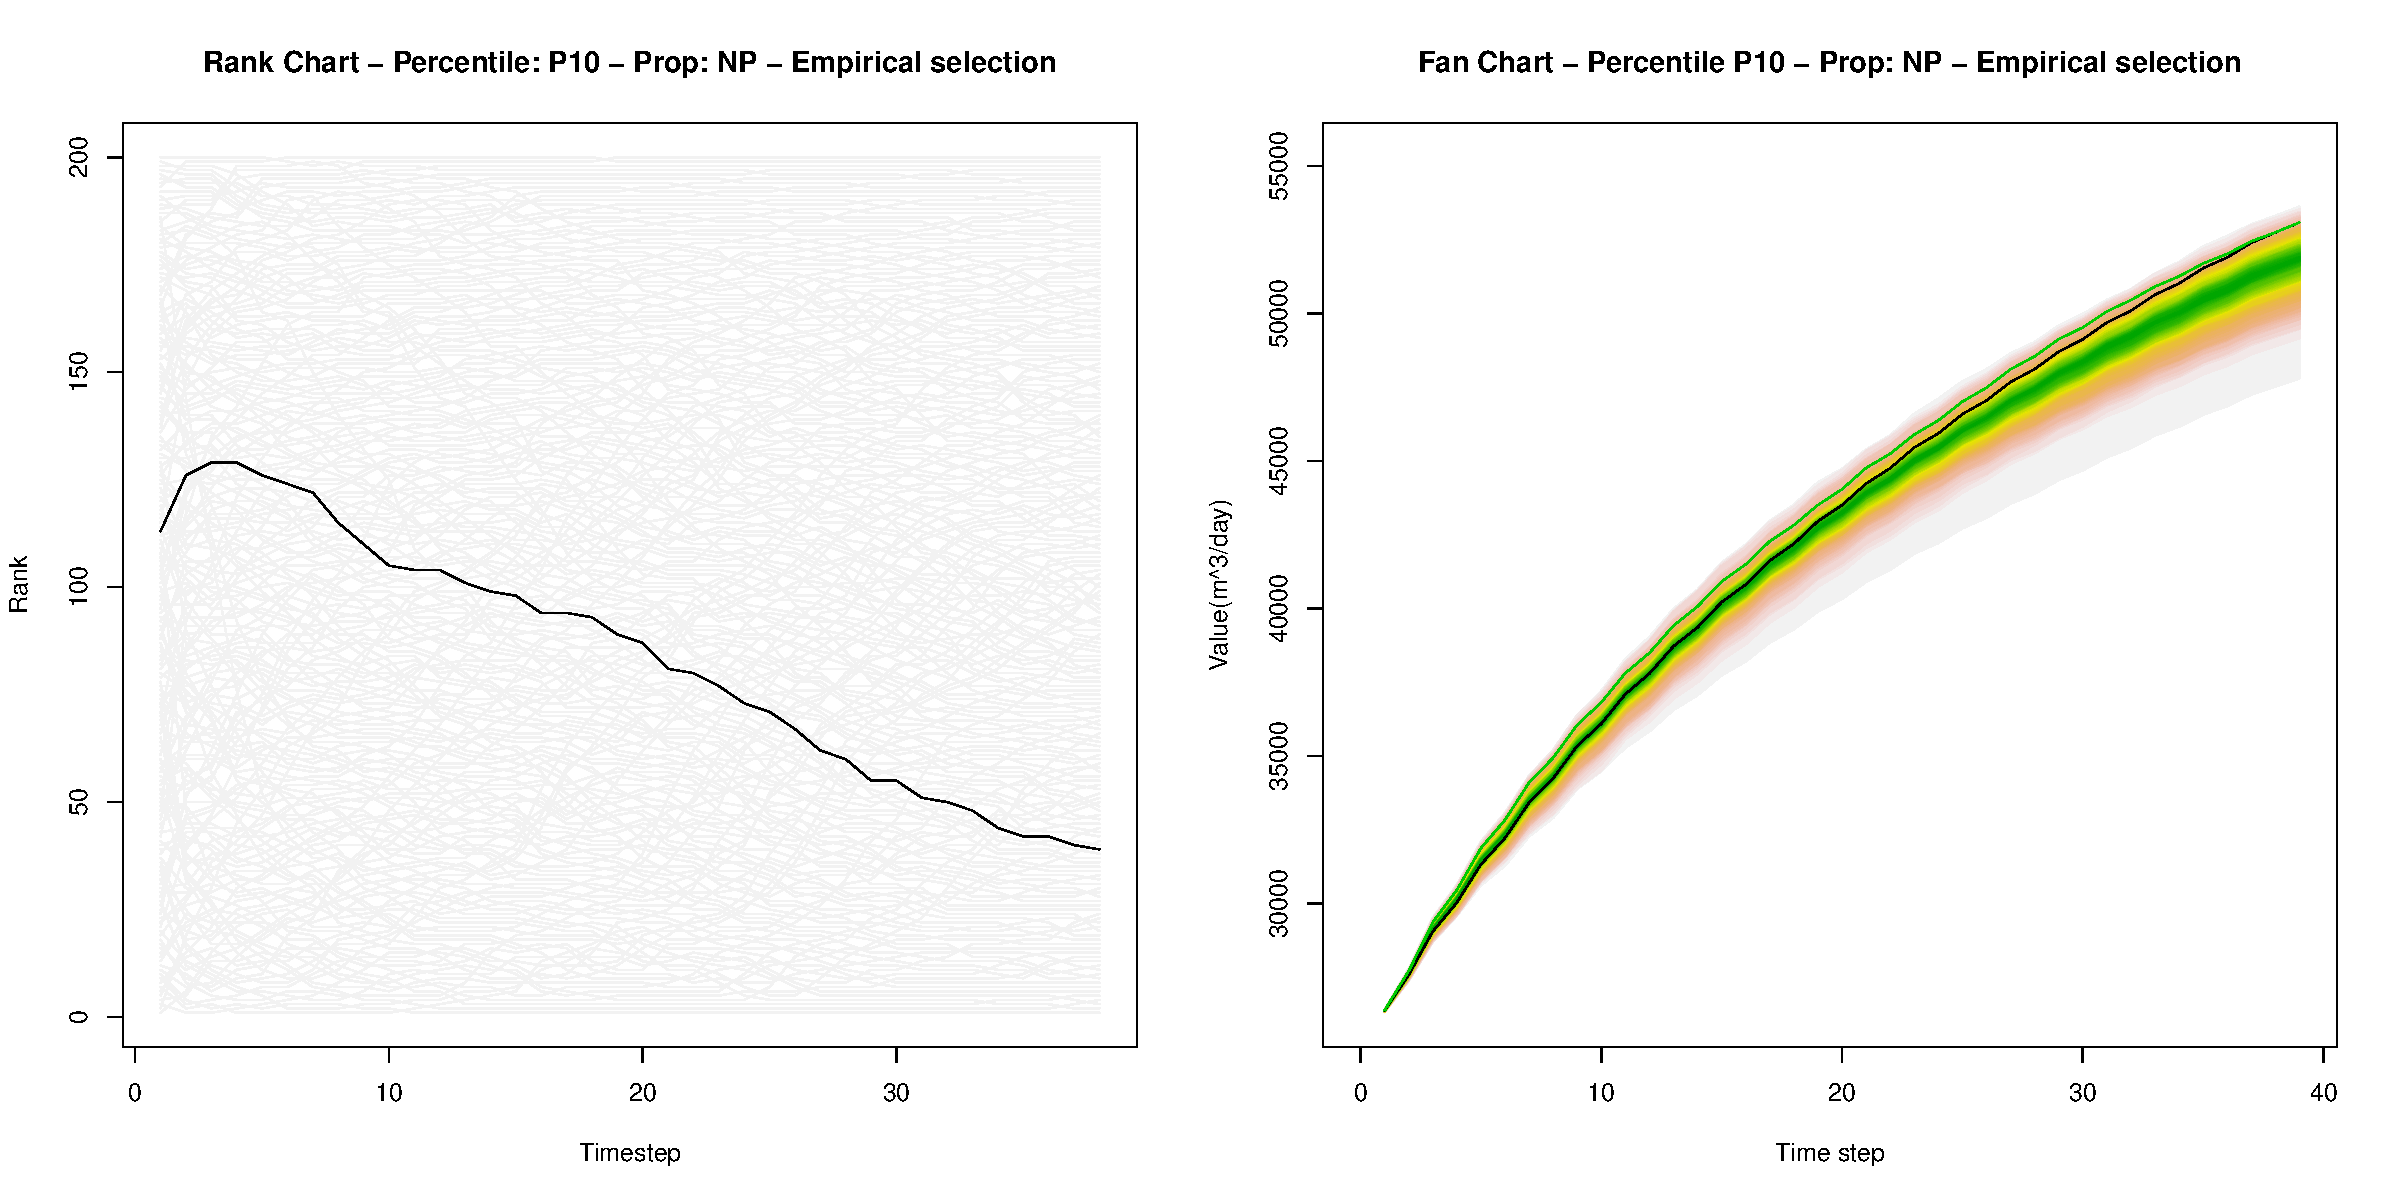
\includegraphics[width=0.85\columnwidth]{rank-fan-ecdf-p10.pdf}
  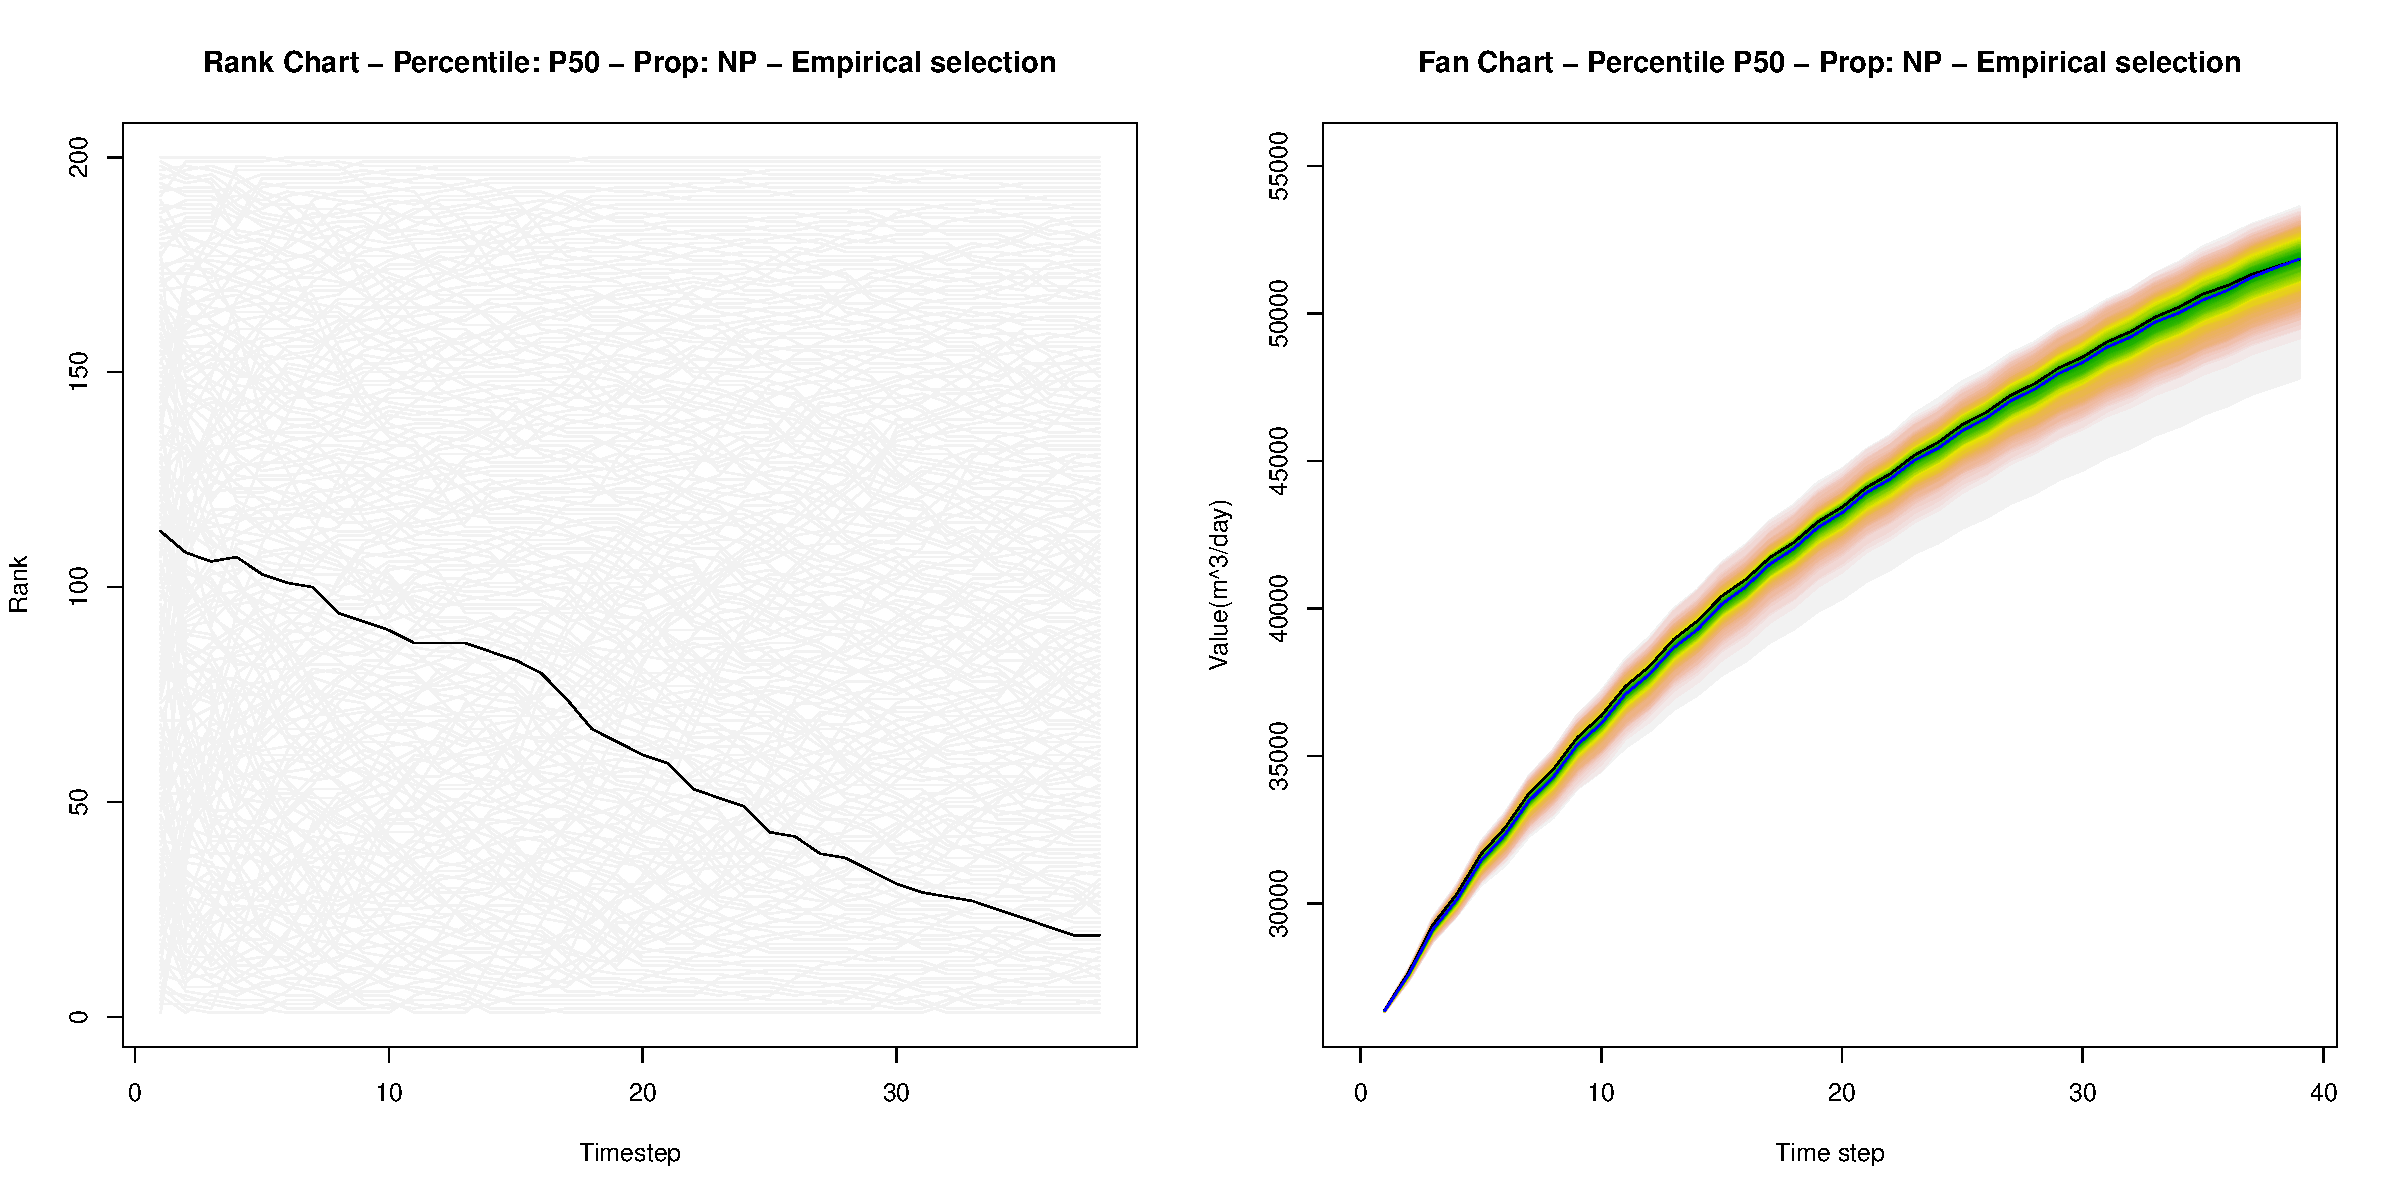
\includegraphics[width=0.85\columnwidth]{rank-fan-ecdf-p50.pdf}
  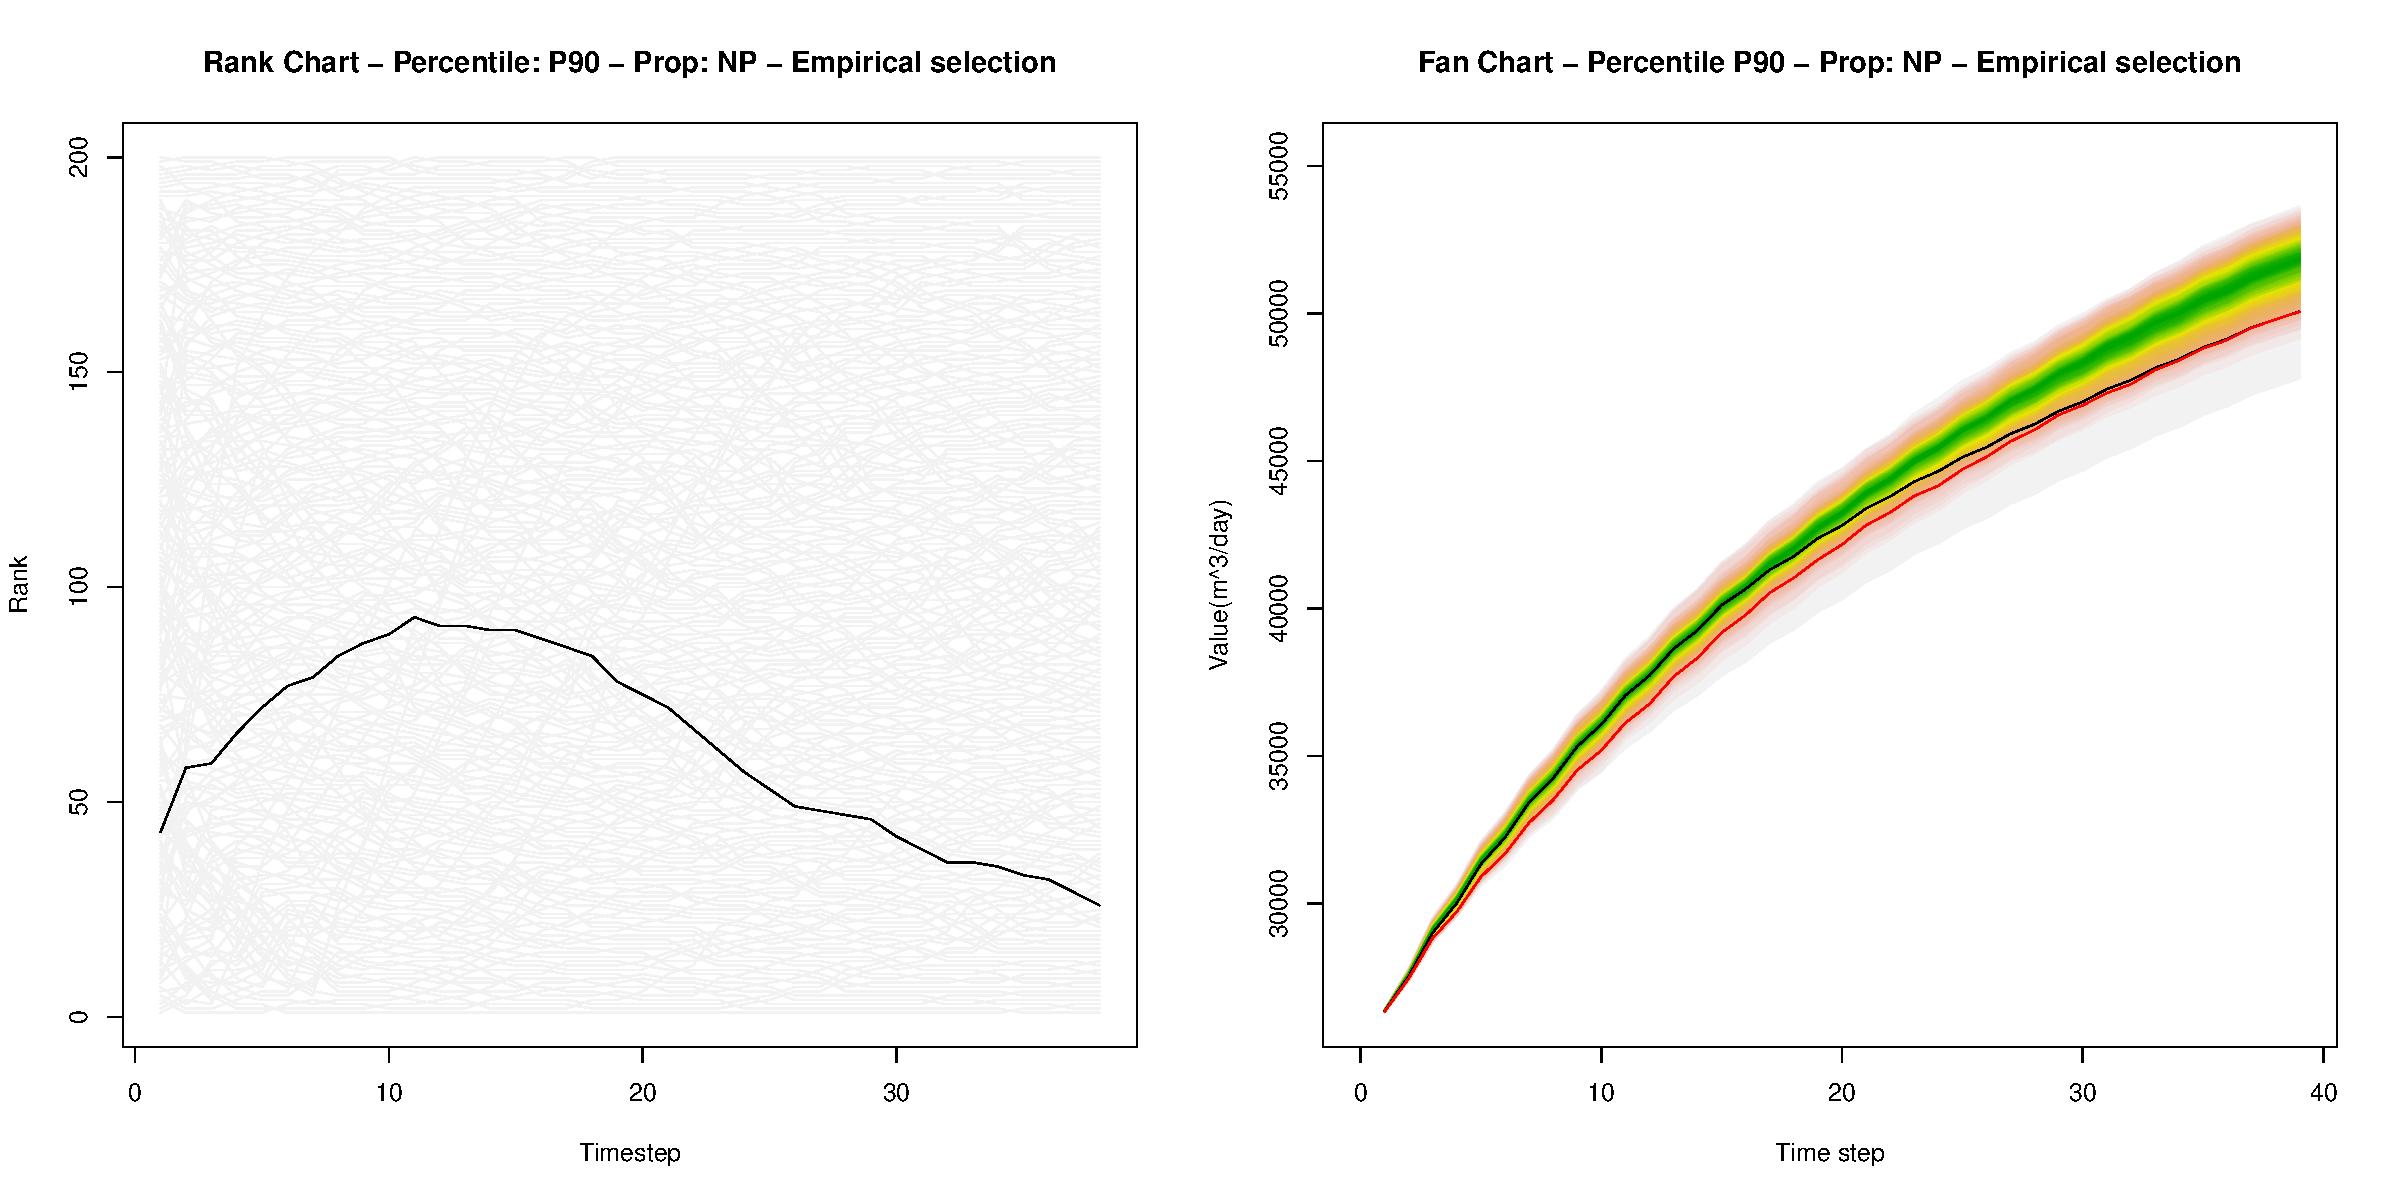
\includegraphics[width=0.85\columnwidth]{rank-fan-ecdf-p90.pdf}
  \caption{Side-by-side rank and fan charts of the models selected using the cumulative probability distribution of the latest production values.}
  \label{fig:rank-fan-ecdf}
\end{figure}

\begin{figure}[H]
  \centering
  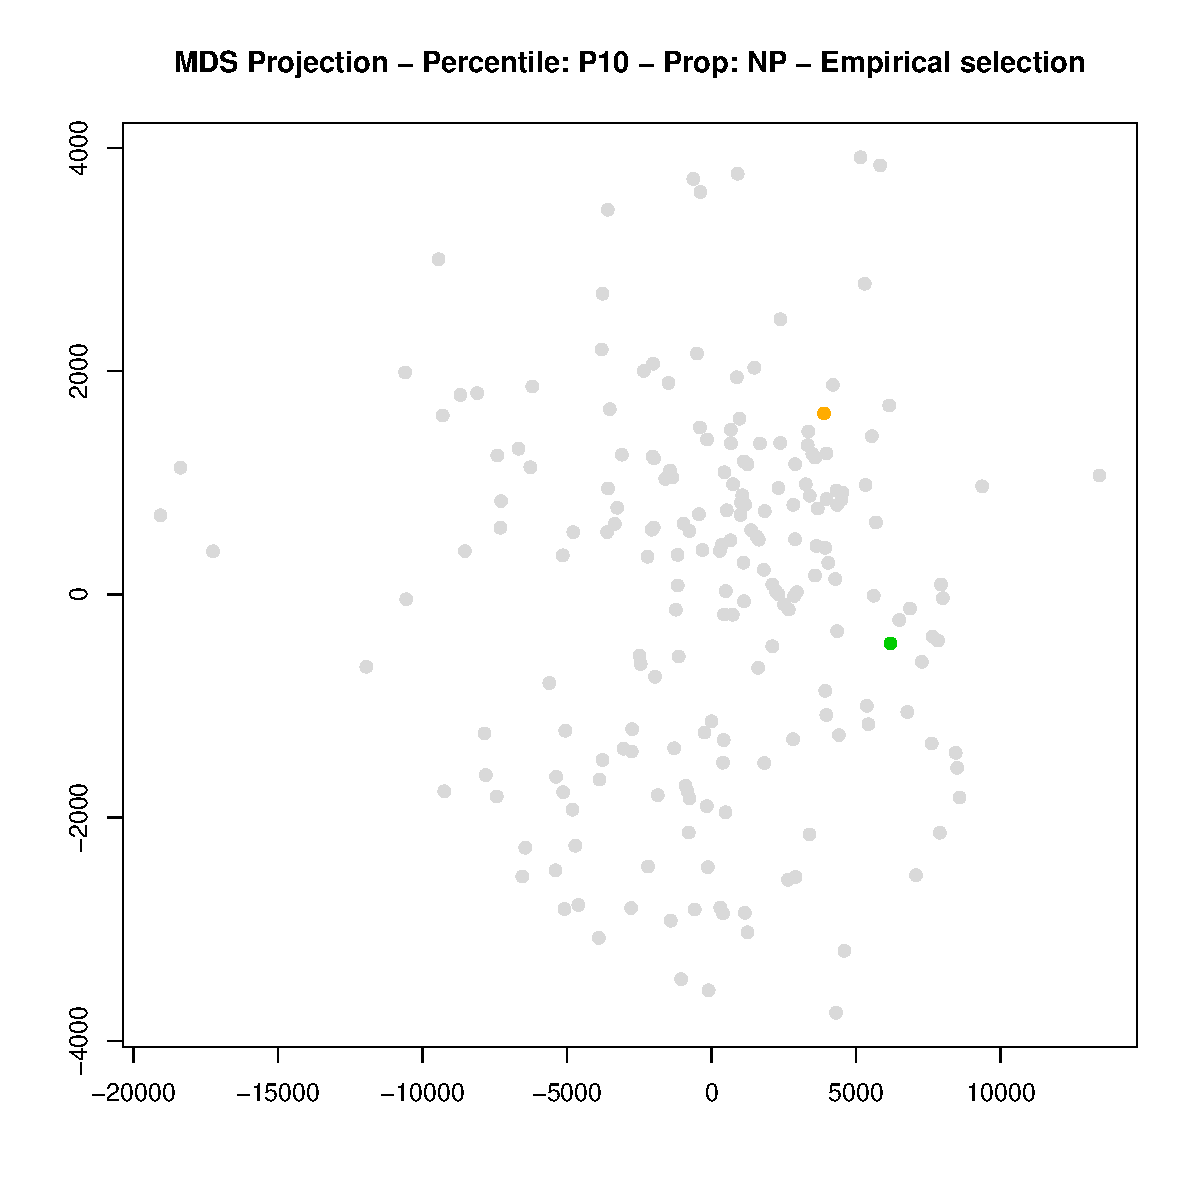
\includegraphics[width=0.49\columnwidth]{mds-ecdf-NP-p10.pdf}
  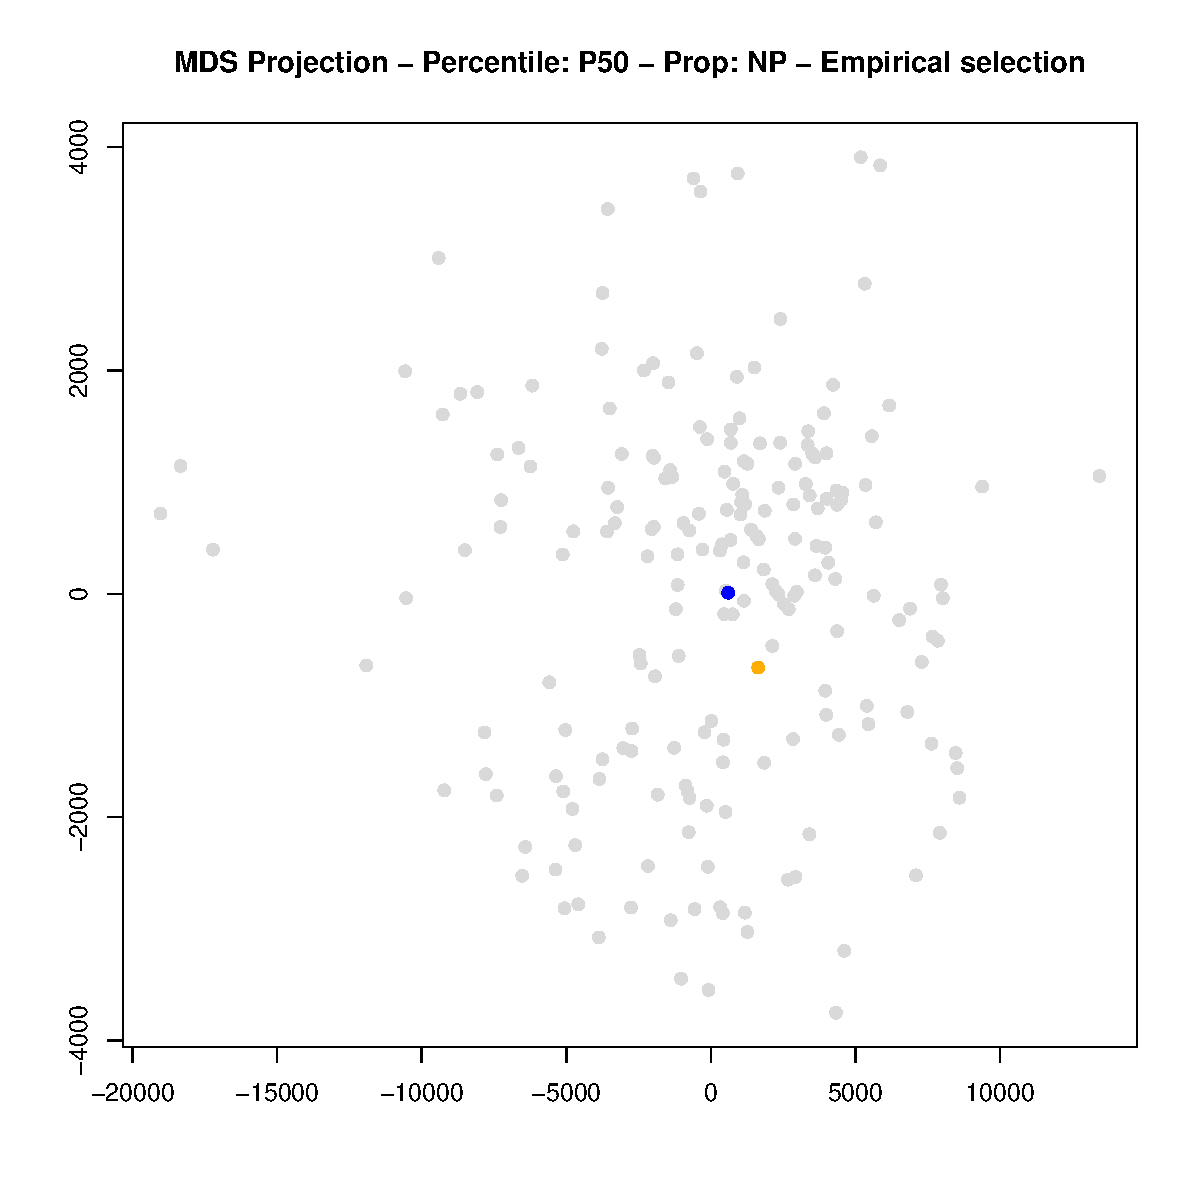
\includegraphics[width=0.49\columnwidth]{mds-ecdf-NP-p50.pdf}
  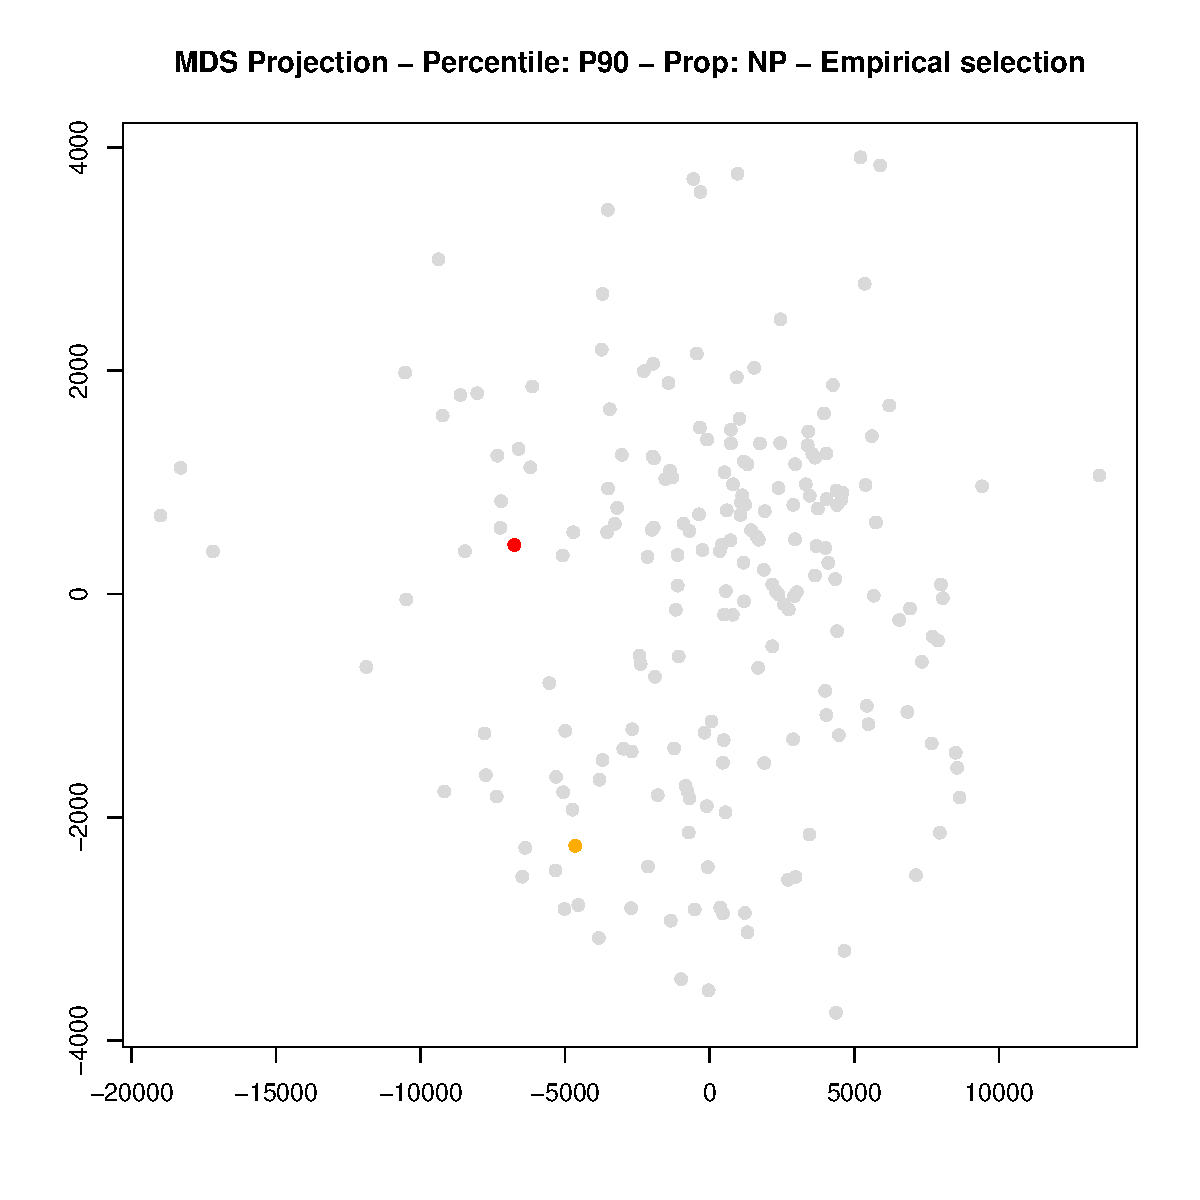
\includegraphics[width=0.49\columnwidth]{mds-ecdf-NP-p90.pdf}
  \caption{MDS projections of the ensemble elements with the selected entities in orange and the P$_{10}$, P$_{50}$ and P$_{90}$ models in green, blue and red respectively.}
  \label{fig:mds-ecdf}
\end{figure}

%The main motivation for our work was the fact that the most relevant works that address the selection issue do not take into account the whole range of production values, only the final ones. Therefore, the resulting models selected by the MinMax \cite{selection-sarma:2013} and Meira et al. \cite{meira:2016} approaches may be representative of the ensemble only in the final production values, not necessarily in the whole range of the simulation. We believe that the lack of consideration towards the model's evolution may lead to poorer selection of representative models.

Our work aims to address this issue by using a range of the estimated production values to select the representative models. We do this by calculating a score prioritizing the general adherence of the models to the reference curves. The adherence itself can be visually analyzed by using the proposed rank chart graphical tool. The rank charts shown as the results of our case study in Section \ref{sec:experiments}, specifically in Figure \ref{fig:rank-plots}, illustrate that the selected models have a very good adherence to the reference curves towards the end of the simulation time. However, a poorer adherence can be noticed at the beginning of the forecasts. Such results may not be easily spotted using the other graphical tools, such as the fan chart. This indicates that the rank chart may be a valuable instrument in analyzing the results of representative selection approaches.

The key issue with our approach is that it takes into account only one property at a time, i.e. cumulative oil production, or the cumulative water production, whereas Sarma et al. and Meira et al. can handle multiple properties of interest at the same time, thus selecting a representative model that satisfies several constraints at once. Adapting our technique to deal with multiple properties is a complex task, since we treat each model as a time series, instead of a scalar value for each property. This adaption would require the use of a composite distance metric to calculate the scores. Since the results obtained with our experiments using an euclidean metric were satisfactory, we saw no need to apply a more sofisticated distance metric. However the euclidean distance is hardly ideal for time series related task and thus, this issue will require further investigation. %The choice of an appropriate metric, while essential to any time series analysis task, is not the goal of our work.

Another issue is that the MinMax approach uses the uncertainty space parameters specific to oil \& gas fields during the step of maximizing the spread of the models. However, this step can be discarded, so that their approach would be a direct application of a simple MinMax technique. In comparison, Meira et al. uses a more complete framework to select the models and define a production strategy for oil \& gas fields, using economic parameters, such as the net present value, besides the petrophysical ones. Our proposed approach uses only the production data itself, no economic or uncertainty parameters, making it readily applicable to other areas of interest. These differences make a direct quantitative comparison of the existing approaches and ours a very difficult, if not an impossible task.

%TODO: Fix this.
%In a visual sense, the models selected by using our score function and the brushing \& linking component are close to the percentile curves during the whole interval, and not only in the end of the simulation. The rank chart provides the means to analyze the adherence of the selected models to each reference percentile. 

%Previous works do not take into consideration the evolution of the system since they deal only with the latest production data. A time series analysis approach is more complex due to the high dimensionality of the problem, requiring a conscious decision regarding the distance metric used and the fact that this metric is usually very specific to the problem and data at hand. These facts make a quantitative comparison of our results with the ones obtained by Sarma et al. \cite{selection-sarma:2013} and Meira et al. \cite{meira:2016} very difficult.

%Sarma's work obtained impressive results, but it is not easily adapted for other areas of interest because it uses uncertainty parameters specific to oil \& gas fields during the step of maximizing the spread of the selected models. However, this step can be discarded and their approach would be a direct application of a single constraint MinMax algorithm. Even so, their approach deals only with scalar data, and does not take into consideration past production values. The past behavior of a system is also important when selecting the most similar models, since it may be possible to analyze if the selected models approached the references only in the end of the simulation or if they were consistently close during the whole interval.

%Meira's work suffers from the very same deficiencies. While it is a much more complete approach when compared to the MinMax algorithm, it still uses only the latest production data in its approach. However, Meira doesn't use only the production data, but also economic value from each reservoir to select the representative models.

%%%%%%%%%%%%%%%%%%%%%%%%%%%%%%%%%%%%%%%%%%%%%%%%%%%%%%%%%%%%%%%%%%%%%%%%%%%%%%

\section{Conclusions}
\label{sec:conclusion}

In this paper, we proposed an approach to select representative models for time series ensembles. To accomplish this task, We  proposed a score function to automatically select a subset of time series as possible candidates for the representative model subset. We tested our score function against the time series manually selected using a brushing \& linking framework with the scenario/distance chart as a graphical tool for the brushing. As far as we know, the scenario/distance chart is not commonly used in practice in this context. Usually engineers employ scatter charts featuring the desired properties, such as NPV $\times$ NP, or WP $\times$ BHP. The results indicate that our approach obtains a good set of possible candidates.

We also developed a graphical tool, named rank chart, in order to evaluate the adherence of ensemble members to a reference curve. When compared to other graphical tools, such as the fan chart and overlaid line chart, the behavior of the ensemble time series could be easily compared to a reference curve even in the presence of a low variance between the curves. After the selection of a subset of possible representatives, the rank chart was an invaluable tool to help analyze their behavior.

When compared to previous works, our approach makes a significant contribution by dealing with a range of production values instead of handling only the final values. The past behavior of a model can significantly impact in the selection task and, thus, it should be taken into consideration. With our work, we also hope to draw attention to this issue and provide the initial milestone to address it. However, our approach considers only one property when selecting the representative models. This may result in a sub-optimal selection when compared to more recent approaches \cite{selection-sarma:2013, meira:2016} that take into account multiple properties and thus select representative models in several aspects.

As future work, we will look for ways to validate our method by interviewing expert users of such systems and comparing our results with results obtained by other algorithms, when available. In the context of oil \& gas industry, we will look for ways to find if the whole time series must be considered, or only a time range deemed important by the users, such as the begining of the forecasts, or the end of the simulation time. We will also study ways to include multivariate time series in our analysis with hopes that it will lead to a better model selection by using more information available from the ensemble. We plan to look for ways of representing such time series in our rank chart, or find an alternative equivalent representation. We will evaluate the possibility of including pre simulation parameters akin to previous works and analyze their impact on the model selection process.

%%%%%%%%%%%%%%%%%%%%%%%%%%%%%%%%%%%%%%%%%%%%%%%%%%%%%%%%%%%%%%%%%%%%%%%%%%%%%%

\section*{Acknowledgements}
The authors would like to thank PETROBRAS for supporting this research. Guilherme Schardong, Waldemar Celes, Simone Barbosa and H\'elio Lopes would like also to thank CNPq for partially supporting their research.

%% The Appendices part is started with the command \appendix;
%% appendix sections are then done as normal sections
%% \appendix

%% \section{}
%% \label{}

%% \newpage

\section*{References}
\bibliographystyle{elsarticle-num} 
\bibliography{references}

\end{document}
\endinput
